\documentclass[a4paper,oneside]{report}
\usepackage{scrextend}
\changefontsizes{13pt}

\usepackage{fontspec}
\usepackage{newtxmath}
\setmainfont{Times New Roman}
\setsansfont{Arial}
\setmonofont{Courier New}

\usepackage[vietnamese]{babel}

\linespread{1.5}
\usepackage{graphicx}
\graphicspath{{images/}}
\usepackage{float}
\usepackage{geometry}
\usepackage{hyperref}
\usepackage{parskip}
\usepackage{amsfonts}
\usepackage{amssymb}
\usepackage{nccmath}
\usepackage{listings}
\usepackage{color}
\usepackage{multirow}
\usepackage{amsmath}
\usepackage{longtable}
\usepackage{multido}
 
\definecolor{dkgreen}{rgb}{0,0.6,0}
\definecolor{gray}{rgb}{0.5,0.5,0.5}
\definecolor{mauve}{rgb}{0.58,0,0.82}

\lstset{frame=tb,
  aboveskip=3mm,
  belowskip=3mm,
  language=Java,
  showstringspaces=false,
  columns=flexible,
  basicstyle={\small\ttfamily},
  numbers=none,
  numberstyle=\tiny\color{gray},
  keywordstyle=\color{blue},
  commentstyle=\color{dkgreen},
  stringstyle=\color{mauve},
  breaklines=true,
  breakatwhitespace=true,
  tabsize=4
}

\geometry{
left=35mm,
right=20mm,
top=30mm,
bottom=30mm
}

\setlength{\parindent}{1.5em}
\setlength{\parskip}{0.5em}

\usepackage{standalone}

\title{
	{Phát hiện và phòng thủ trước các cuộc tấn công từ chối dịch vụ dựa trên các phương thức học máy và học sâu trong Software-defined Networking }\\
	{\large FIT - HCMUS}\\
}
\author{Author Name}
\date{day month year}

\usepackage{fancyhdr}
\pagestyle{fancy}
\fancyhf{}
\setlength{\headheight}{13pt}
\rhead{\nouppercase\leftmark}
\cfoot{\thepage}

\usepackage{array}
\newcolumntype{P}[1]{>{\centering\arraybackslash}p{#1}}

\usepackage{cite}
%\addbibresource{thesis.bib}
\usepackage{fancybox}
\usepackage{setspace}

\begin{document}

%bia ngoai
\begin{titlepage} 
\thisfancypage{
\setlength{\fboxsep}{10pt}
\doublebox
}{}
\begin{center}
\begin{large}
TRƯỜNG ĐẠI HỌC KHOA HỌC TỰ NHIÊN\\
KHOA CÔNG NGHỆ THÔNG TIN\\
LỚP CỬ NHÂN TÀI NĂNG \\
\end{large}
\vskip1cm
\vskip1.5cm
\begin{large}
%\bfseries
LƯƠNG TẤN KHANG\\
\end{large}
\vskip3cm
\begin{Large}
\bfseries
\onehalfspacing
PHÁT HIỆN VÀ PHÒNG THỦ TRƯỚC CÁC CUỘC TẤN CÔNG TỪ CHỐI DỊCH VỤ TRONG SOFTWARE-DEFINED NETWORKING DỰA TRÊN CÁC PHƯƠNG THỨC HỌC MÁY VÀ HỌC SÂU
\end{Large}
\vskip4cm
\begin{large}
KHÓA LUẬN TỐT NGHIỆP CỬ NHÂN CNTT \\
\end{large}
\vskip5cm
\begin{normalsize}
TP.HCM, NĂM 2020
\end{normalsize}
\end{center}
\end{titlepage}

%bia trong
\begin{titlepage} 
\thisfancypage{
\setlength{\fboxsep}{10pt}
\doublebox
}{}
\begin{center}
\begin{large}
TRƯỜNG ĐẠI HỌC KHOA HỌC TỰ NHIÊN\\
KHOA CÔNG NGHỆ THÔNG TIN\\
LỚP CỬ NHÂN TÀI NĂNG \\
\end{large}
\vskip1cm
\vskip1.5cm
\begin{large}
%\bfseries
LƯƠNG TẤN KHANG - 1612865 \\
\end{large}
\vskip2cm
\begin{Large}
\bfseries
\onehalfspacing
PHÁT HIỆN VÀ PHÒNG THỦ TRƯỚC CÁC CUỘC TẤN CÔNG TỪ CHỐI DỊCH VỤ TRONG SOFTWARE-DEFINED NETWORKING DỰA TRÊN CÁC PHƯƠNG THỨC HỌC MÁY VÀ HỌC SÂU
\end{Large}
\vskip1.5cm
\begin{large}
KHÓA LUẬN TỐT NGHIỆP CỬ NHÂN CNTT \\
\end{large}
\vskip1cm
\begin{large}
GIÁO VIÊN HƯỚNG DẪN \\
\textbf{TS. TRẦN TRUNG DŨNG} \\
\textbf{ThS. LÊ GIANG THANH} \\
\end{large}

\vskip4cm
\begin{normalsize}
KHÓA 2016 - 2020
\end{normalsize}
\end{center}
\end{titlepage}

\newcommand{\Pointilles}[1]{%
	\par\nobreak
	\noindent\rule{0pt}{1.5\baselineskip}
	\multido{}{#1}{\noindent\makebox[\linewidth]{\dotfill}\endgraf} ...
	\bigskip%
}
	
\begin{titlepage}
	\begin{center}
		\begin{large}
			NHẬN XÉT CỦA GIÁO VIÊN HƯỚNG DẪN
		\end{large}
	\end{center}
\Pointilles{17}
\begin{center}
	\raggedleft\textnormal{Tp.HCM, Ngày .... tháng .... năm 2020} \hfill \\
	\raggedleft\textbf{Giáo viên hướng dẫn}\hspace{1.5cm} \hfill
\end{center}
\end{titlepage}

\begin{titlepage}
	\begin{center}
		\begin{large}
			NHẬN XÉT CỦA GIÁO VIÊN PHẢN BIỆN
		\end{large}
	\end{center}
	\Pointilles{16}
	
Khóa luận đáp ứng yêu cầu của Khóa luận cử nhân CNTT.

	\begin{center}
		\raggedleft\textnormal{Tp.HCM, Ngày .... tháng .... năm 2020} \hfill \\
		\raggedleft\textbf{Giáo viên phản biện}\hspace{1.5cm} \hfill
	\end{center}
\end{titlepage}
	


\pagenumbering{roman}

\chapter*{Lời cảm ơn}
\markboth{Lời cảm ơn}{Lời cảm ơn}
Để hoàn thành khóa luận này tôi tỏ lòng biết ơn sâu sắc đến thầy TS. Trần Trung Dũng và thầy
ThS. Lê Giang Thanh. Các thầy đã tận tình giúp tôi trong suốt
quá trình nghiên cứu và hoàn thành khóa luận này.

Tôi chân thành cảm ơn quý thầy cô trong trường Đại học Khoa học Tự nhiên thành phố Hồ Chí
Minh đã giảng dạy và truyền đạt kiến thức cho tôi trong suốt quãng thời gian học tập và
nghiên cứu ở trường.

Tôi xin dành lời cảm ơn riêng cho thầy cô khoa Công nghệ thông tin đã tạo
điều kiện cơ sở vật chất cho tôi có thể tiến hành các nghiên cứu và thí nghiệm tại phòng
bộ môn Mạng máy tính.

\begin{flushright}
\textit{Sinh viên thực hiện}
\end{flushright}

\tableofcontents

\chapter*{Danh mục từ khóa}
\markboth{Danh mục từ khóa}{Danh mục từ khóa}
\begin{tabular}{p{3cm}l}
CNN & Convolutional Neural Network \\
DDoS & Distributed Denial of Service \\
DoS & Denial of Service \\
DNN & Deep neural Network \\
DT & Decision Tree \\
IDS & Intrusion Detection Systems \\
IoT & Internet of Things \\
LSVM & Linear Support Vector Machine \\
NB & Naïve Bayes \\
NN & Neural Network \\
ReLU & Rectified linear unit \\
RF & Random forests \\
RNN & Recurrent neural network \\
SDN & Software-Defined Networking \\
SVM & Support Vector Machine  \\
\end{tabular}

\listoffigures

\listoftables

\chapter*{Lời mở đầu}
\pagenumbering{arabic} 
\addcontentsline{toc}{chapter}{Lời mở đầu}
\markboth{Lời mở đầu}{Lời mở đầu}
\label{chap:foreword}
Trong thời đại phát triển nhanh chóng của Internet hiện nay, các phương thức bảo mật và an toàn thông tin đang ngày càng được chú trọng. Trong đó, tấn công từ chối dịch vụ (DoS) và tấn công từ chối dịch vụ phân tán (DDoS) đang trở thành mối đe dọa lên toàn thể các máy chủ trên thế giới. Từ đó, các phương thức và dịch vụ phòng chống, giảm thiểu thiệt hại cũng được ra mắt với rất nhiều các chức năng khác nhau.

Một số vấn đề nổi trội khi thực hiện phòng thủ trước tấn công DoS/DDoS đó chính là chi phí cài đặt và vận hành hệ thống khá tốn kém. Bên cạnh đó, các phương pháp tấn công ngày càng đa dạng với quy mô ngày một lớn, khiến cho các phương pháp phòng chống nhanh chóng trở nên lỗi thời và bị vô hiệu hóa. Trong khóa  luận này, tôi hi vọng có thể giải quyết được các vấn đề trên, cung cấp một giải pháp phòng thủ trước tấn công DoS/DDoS trong mạng Software defined network (SDN) hợp lý, gọn nhẹ và dễ dàng triển khai.

Tôi đã tiến hành tìm hiểu các nghiên cứu học thuật cũng như một số các sản phẩm liên quan đến vấn đề này trên thị trường. Từ đó, xem xét khả năng ứng dụng học sâu và học máy vào giải pháp phát hiện tấn công DoS/DDoS. Sau đó tôi thiết kế và xây dựng một proof-of-concept cho phần mềm nhận diện tấn công DoS/DDoS và một proof-of-concept cho hệ thống triển khai trong mạng SDN.

Văn bản này trình bày tổng kết lại quá trình tìm hiểu và xây dựng Hệ thống phát hiện và phòng thủ trước các cuộc tấn công từ chối dịch vụ và từ chối dịch vụ phân tán trong môi trường mạng SDN. Toàn bộ văn bản được chia thành các chương với nội dung như sau:

\textbf{Chương \ref{chap:introduction}. Giới thiệu}

Trình bày chi tiết nguyên nhân và động lực của tôi khi thực hiện khóa luận này, cũng như mục tiêu đặt ra và hướng tiếp cận của tôi đối với vấn đề.

\textbf{Chương \ref{chap:background}. Cơ sở lý thuyết}

Trình bày những khái niệm cơ bản, giúp người đọc có cái nhìn tổng quan về cơ sở lý thuyết của khóa luận cũng như làm nền tảng cho những chương tiếp theo.

\textbf{Chương \ref{chap:review}. Các công trình liên quan}

Trình bày những tìm hiểu của tôi về các nghiên cứu phát hiện và phòng thủ trước tấn công DoS/DDoS đã có. Tìm ưu nhược điểm trong các nghiên cứu này.

\textbf{Chương \ref{chap:method}. Mô hình giải pháp của đề tài}

Trình bày và giới thiệu giải pháp của tôi đề xuất cho một hệ thống phát hiện và phòng thủ trước tấn công DoS/DDoS.

\textbf{Chương \ref{chap:network_model}. Mô hình mạng thử nghiệm}

Áp dụng giải pháp đề xuất ở chương 4 vào mạng SDN trong môi trường mạng thử nghiệm.

\textbf{Chương \ref{chap:testing}. Thử nghiệm và phân tích kết quả}

Kiểm lỗi và độ chính xác của hệ thống khi áp dụng vào mạng SDN

\textbf{Chương \ref{chap:conclusion}. Tổng kết}

Tổng kết lại quá trình thực hiện khóa luận, những điểm đạt và chưa đạt, đồng thời đề xuất hướng phát triển trong tương lai. 

\chapter{Giới thiệu}
\label{chap:introduction}
\section{Tổng quan về đề tài}
Phát hiện và phòng thủ trước tấn công DoS/DDoS không phải là một lĩnh vực mới. Kể từ khi cuộc tấn công DDoS lần đầu tiên xuất hiện vào năm 1999, thì tấn công DDoS đang ngày càng trở nên đa dạng và phức tạp. Từ đó, loại tấn công mạng này được xem như là một vấn nạn, một mối đe dọa rất lớn đối với các hệ thống mạng và hệ thống máy chủ trên thế giới. Phát hiện tấn công DoS/DDoS theo đánh giá của các chuyên gia và các tổ chức an ninh mạng hiện nay là bài toán rất khó. Nguyên nhân là vì các cách thức và các cuộc tấn công ngày càng đa dạng và xuất hiện với mức độ dày đặc. Bên cạnh đó, với nền tảng vạn vật kết nối (IoT) phát triển mạnh mẽ, nhu cầu về một mạng lưới đa năng và uyển chuyển dẫn đến sự áp dụng mạnh mẽ Software Defined Network (SDN) vào nền tảng này. Từ đó, phát hiện tấn công DoS/DDoS trong SDN đang là đề tài được chú trọng và nhiều người nghiên cứu.

Các phương thức phát hiện tấn công DDoS hiện nay chủ yếu hiện nay dựa trên việc theo dõi mật độ dữ liệu di chuyển trong hệ thống mạng. Với phương pháp này, việc nhận diện hệ thống đang bị tấn công mật độ cao (high-rate) rất dễ dàng. Tuy nhiên, phương pháp này dễ bị nhầm lẫn giữa tấn công với quá tải do nhu cầu sử dụng tăng cao đột ngột và rõ ràng là không hiệu quả trong việc phát hiện tấn công mật độ thấp (low-rate). Hiện nay, trong môi trường SDN, phương pháp theo dõi này được áp dụng chủ yếu, ở đó, người ta sẽ theo dõi các dữ liệu thống kê các luồng mở do các thiết bị OpenFlow switch trả về. Bên cạnh đó, các phương pháp thống kê và phân tích luồng dữ liệu cũng được áp dụng rộng rãi. Đây là phương pháp được đánh giá tốt hiện nay, tuy nhiên, để có thể chọn được các đặc trưng thống kê và phân tích hiệu quả, phương pháp này cần một người nghiên cứu có trình độ về thống kê nhất định. Ngoài ra, mỗi khi áp dụng các phương pháp thống kê và phân tích mới, các nhà nghiên cứu phải bỏ công sức làm lại từ đầu, từ đó dẫn đến tốn kém về mặt thời gian và nhân lực. 

Hiện nay, các nghiên cứu áp dụng học máy và học sâu trong phát hiện tấn công DoS/DDoS đang xuất hiện ngày một nhiều với các thành tựu đáng kể. Hai phương pháp này đã cho thấy khả năng nhận diện tấn công vượt trội của mình. Từ đó đã thúc đẩy tôi nghiên cứu một hệ thống phát hiện tấn công DoS/DDoS dựa trên nền tảng của các nghiên cứu học máy và học sâu trước đó. Sau đó áp dụng vào hệ thống mạng SDN để có thể phát hiện sớm tấn công DoS/DDoS và giảm thiểu thiệt hại do nó gây ra. Sau cùng, để kiểm thử hệ thống, tôi xây dựng lên hai kịch bản phòng thủ quan trọng: phòng thủ từ nguồn tấn công và phòng thủ từ tấn công bên ngoài.

\section{Bài toán nghiên cứu của đề tài}

Trong khóa luận này, hai mục tiêu chính mà tôi hướng đến là nhận diện và phòng thủ trước tấn công DoS/DDoS trong môi trường mạng SDN.

Trong bài toán nhận diện, tôi áp dụng các phương pháp, các mô hình học máy và học sâu đã được nghiên cứu trước đó để tìm ra được mô hình tốt nhất, cũng như đánh giá ưu và nhược điểm của các mô hình trong các hoàn cảnh khác nhau. Áp dụng huấn luyện nhiều mô hình, tôi tìm ra được mô hình học  máy có hướng tiếp cận  đơn giản  mà kết quả thu được lại tốt nhất là mô hình Decision Tree.

Trong bài toán phòng thủ, tận dụng tính uyển chuyển và tính tập trung của mạng SDN, tôi đề xuất một giải pháp đơn giản mà hiệu quả trong việc ngăn chặn các luồng tấn công DDoS được chẩn đoán từ mô hình học  máy và học sâu.

Kết hợp hai mục tiêu trên, tôi xây dựng nên một hệ thống nhận diện và phòng thủ toàn diện trước tấn công DoS/DDoS trong môi trường mạng SDN.

\section{Mục tiêu đặt ra và hướng tiếp cận vấn đề}

Những mục tiêu mà chúng tôi muốn đạt được như sau:

\begin{itemize}
\item[--] Hoàn thành thành một phần mềm proof-of-concept trong việc phân loại tấn công DoS/DDoS.
\item[--] Triển khai một hệ thống phòng thủ proof-of-concept trong mạng SDN.
\item[--] Huấn luyện trên các mô hình học máy và học sâu khác nhau.
\item[--] Dễ dàng thay đổi mô hình nhận diện tấn công trong hệ thống.
\item[--] Dễ dàng mở rộng và áp dụng vào các nền tảng mạng khác so với SDN.
\item[--] Bảo đảm phần mềm có thể hoạt động theo thời gian thực trên một hệ phần cứng cơ bản.
\item[--] Cung cấp giao diện thống kê lưu lượng mạng theo thời gian thực trên nền tảng web.
\end{itemize}


Từ những mục tiêu trên, hướng tiếp cận của chúng tôi như sau:

\begin{itemize}
\item[--] Tập trung xây dựng hệ thống nhận diện và phòng thủ cơ bản, sau đó mới tối ưu hóa sau.
\item[--] Ưu tiên sử dụng các mô hình học máy và học sâu đơn giản mà hiệu quả.
\item[--] Ưu tiên sử dụng những công cụ mô phỏng mạng SDN gọn nhẹ.
\end{itemize}

\section{Đối tượng nghiên cứu}

Những đối tượng nghiên cứu chính trong khóa luận này bao gồm:

\begin{itemize}
\item[--] Lý thuyết và cách thức tấn công từ chối dịch vụ và từ chối dịch vụ phân tán.
\item[--] Lý thuyết và mô hình máy học và học sâu.
\item[--] Lý thuyết và ứng dụng mạng Software defined network.
\item[--] Các tập dữ liệu về tấn công DoS/DDoS đang có hiện nay.
\item[--] Các giải pháp phát hiện tấn công DoS/DDoS bằng các phương pháp học máy và học sâu.
\item[--] Các giải pháp phát hiện và phòng thủ trước tấn công DoS/DDoS trong mạng SDN.
\end{itemize}

Trên đây là toàn bộ nội dung của chương \ref{chap:introduction} của khóa luận. Qua những gì đã trình bày, tôi hy vọng có thể giúp người đọc có được cái nhìn tổng quát nhất về những vấn đề còn tồn đọng, nguyên nhân, động lực đã thúc đẩy tôi bắt tay vào thực hiện khóa luận này. Bên cạnh đó, tôi cũng đã trình bày những mục tiêu, hướng tiếp cận mà tôi đã vạch ra trước khi bước vào việc tìm hiểu những đối tượng nghiên cứu chính.

Trong chương tiếp theo, tôi sẽ trình bày cơ sở lý thuyết và các khái niệm cơ bản nhất về tấn công từ chối dịch vụ và từ chối dịch vụ phân tán, học máy, học sâu và mạng SDN, giúp người dùng có cái nhìn tổng quan về lý thuyết, dễ nắm bắt hơn khi đọc khóa luận này.

\chapter{Cơ sở lý thuyết}
\label{chap:background}
\section{Tấn công từ chối dịch vụ (DoS) và tấn công từ chối dịch vụ phân tán (DDoS)}

\subsection{Tấn công từ chối dịch vụ}

\subsubsection{Tấn công từ chối dịch vụ là gì?}

Theo định nghĩa của \cite{1-dos-concept}, một cuộc tấn công từ chối dịch vụ diễn ra khi người dùng hợp lệ không có khả năng truy cập thông tin từ các hệ thống, các thiết bị hoặc các tài nguyên mạng do sự can thiệp của nhân tố mạng độc hại. Những dịch vụ bị ảnh hưởng bao gồm thư điện tử, các trang mạng, các tài khoản trực tuyến (ví dụ như ngân hàng), hay các dịch vụ khác dựa trên tài nguyên máy tính hoặc tài nguyên mạng. Tình trạng ''từ chối dịch vụ''  là khi hệ thống hay mạng lưới của nạn nhân bị làm ngập lụt cho đến lúc không còn khả năng phản hồi, sụp đổ, hay ngăn chặn sự truy cập từ những người dùng hợp lệ. Tấn công từ chối dịch vụ có thể gây hại cho các tổ chức cả về tiền bạc lẫn thời gian trong lúc dịch vụ của họ không thể truy cập được.

Có rất nhiều phương thức để thực hiện tấn công DoS. Phương thức thông thường diễn ra là khi kẻ tấn công làm ngập lụt mạng lưới hệ thống với lưu lượng. Với phương thức này, kẻ tấn công gửi hàng loạt yêu cầu đến máy chủ nạn nhân, làm cho nó quá tải. Những yêu cầu dịch vụ này là bất hợp lệ và có địa chỉ giả mạo, sẽ gây nhầm lẫn cho máy chủ khi nó cố gắng xác thực người gửi yêu cầu. Khi những yêu cầu thừa thải được xử lý liên tục, máy chủ sẽ bị quá tải, từ đó tạo nên trạng thái từ chối dịch vụ đối với các yêu cầu hợp lệ.

\subsubsection{Những loại tấn công DoS thường gặp}

Trong tấn công Smurf \cite{1-dos-concept}, những kẻ tấn công gửi các gói tin broadcast ICMP đến một số lượng đáng kể các máy chủ với các địa chỉ IP nguồn giả mạo, thứ thuộc về máy chủ nạn nhân. Các máy chủ nhận những gói tin này sẽ phản hồi và từ đó làm ngập lụt máy chủ nạn nhân với những gói tin phản hồi này.

Tấn công ngập lụt gói tin SYN \cite{1-dos-concept} diễn ra khi một kẻ tấn công gửi một yêu cầu để kết nối đến máy chủ nạn nhân nhưng lại không hoàn thành kết nối đó thông qua việc bắt tay ba bước – một phương thức được dùng trong mạng lưới TCP/IP để tạo kết nối giữa máy chủ và máy khách. Việc không hoàn thành kết nối sẽ dẫn tới cổng kết nối giữ trạng thái ''bị chiếm giữ'' và không khả dụng cho các kết nối sau này. Kẻ tấn công cứ liên tiếp tạo các kết nối, chiếm giữ tất cả các cổng và từ đó ngăn chặn những người dùng hợp lệ có thể tạo các kết nối mới.

Những mạng lưới cá nhân có thể bị ảnh hưởng bởi các tấn công DoS mà không phải là mục tiêu trực tiếp. Nếu nhà cung cấp dịch vụ Internet hoặc nhà cung cấp dịch vụ đám mây bị nhắm đến và bị tấn công, thì mạng lưới cũng sẽ trải qua việc mất dịch vụ.

Tấn công ngập lụt UDP \cite{2-imperva} diễn ra dựa trên sự không tin cậy của kết nối UDP. Trong tấn công này, rất nhiều gói tin UDP với các cổng ngẫu nhiên được gửi tới nạn nhân. Khi nạn nhân nhận gói tin tại một cổng, nó sẽ tìm kiếm ứng dụng đang lắng nghe cổng đó. Khi nó không tìm được, nó sẽ phản hồi với một gói tin ICMP báo lỗi. Khi một lượng lớn gói tin UDP độc hại được nhận, nạn nhân sẽ tiêu thụ rất nhiều tài nguyên trong việc phản hồi với các gói tin ICMP. Điều này sẽ ngăn chặn nạn nhân phản hồi những người dùng hợp lệ.
 
Slowris \cite{2-imperva} là loại tấn công cho phép một máy tính làm sập các máy chủ web chỉ với một lượng băng thông nhỏ nhưng lại không ảnh hưởng đến các dịch vụ khác của nạn nhân. Slowris thực hiện việc này bằng cách giữ càng nhiều kết nối đến máy chủ web nạn nhân càng lâu càng tốt. Nó sẽ tạo kết nối đến với máy chủ web nạn nhân, tuy nhiên nó chỉ gửi một phần của yêu cầu. Nó liên tục gửi các HTTP header nhưng không bao giờ hoàn thành chúng. Nạn nhân sẽ liên tục giữ những kết nối độc hại này được mở, từ đó dẫn đến quá tải giới hạn kết nối, dẫn đến việc từ chối dịch vụ tới các người dùng hợp lệ.

\subsection{Tấn công từ chối dịch vụ phân tán}

\subsubsection{Tấn công từ chối dịch vụ phân tán là gì?}

Có rất nhiều định nghĩa tấn công DDoS từ các nghiên cứu khác nhau, tuy nhiên chung quy đều có chung suy nghĩ và ý nghĩa.
Theo như \cite{1-dos-concept}, tấn công từ chối dịch vụ diễn ra khi nhiều máy tính vận hành cùng lúc với nhau để tấn công vào một mục tiêu. Những kẻ tấn công thường tận dụng mạng lưới Botnet – một nhóm các thiết bị truy cập Internet bị chiếm giữ - để dẫn tới một tấn công quy mô lớn. Những kẻ tấn công sẽ tìm kiếm và chiếm giữa  các mạng lưới hay thiết bị kết nối Internet có bảo mật kém, từ đó tạo nên mạng Botnet. Tấn công DDoS tạo một lượng yêu cầu cực lớn đến nạn nhân, từ đó gia tăng sức mạnh tấn công, đồng thời rất khó để phòng thủ bởi tính đa dạng và rộng khắp từ các nguồn tấn công.

Nam-Seok Ko và các cộng sự \cite{3-Ko} giải thích rằng tấn công DDoS là sự kết hợp của việc sử dụng một lượng cực lớn lưu lượng mạng bởi kẻ tấn công nhắm vào hệ thống mục tiêu thông qua việc vận hành đồng thời một lượng lớn máy tính được phân tán trên Internet. Theo như nghiên cứu này, lưu lượng tấn công sẽ ngăn cản người dùng thực tế truy cập vào tài nguyên của nạn nhân bằng việc thâu tóm tất cả băng thông mạng và tài nguyên bên trong hệ thống.

Fallah và các cộng sự \cite{4-Fallah} thì cho rằng, tấn công DDoS bắt đầu bằng việc kẻ tấn công sẽ truy tìm các máy chủ có các lỗi bảo mật trên Internet, để có thể xâm nhập và điều khiển chúng gửi một lượng lớn các gói tin đến máy chủ nạn nhân. Hơn nữa, khi kẻ tấn công thành công, chúng đã có thể sử dụng toàn bộ tài nguyên máy chủ như CPU, stack space trong giao thức phần mềm, hoặc Internet link capacity, từ đó nạn nhân không thể cung cấp dịch vụ đến với người dùng thực tế của nó.

Từ góc nhìn của doanh nghiệp, Yoon \cite{5-Yoon} giải thích rằng tấn công DDoS được thể hiện bằng việc kẻ tấn công bên ngoài trên Internet sử dụng BotMaster điều khiển từ xa các Botnet nhằm thực hiện tấn công vào các trang web quan trọng từ đó các dịch vụ kinh doanh thiết yếu như Internet banking, e-government, e-trading, e-commerce, vv, bị vô hiệu hóa đối với người dùng.

Theo \cite{1-dos-concept}, các cuộc tấn công DDoS đã gia tăng cường độ khi ngày càng có nhiều thiết bị IoT ra đời. Các thiết bị IoT thường sử dụng mật khẩu mặc định và không được bảo mật kỹ càng khiến chúng rất dễ bị xâm nhập và khai thác. Việc lây nhiễm các thiết bị IoT thường không được nhiều người chú ý, kẻ tấn công có thể xâm nhập và điều khiển hàng trăm nghìn thiết bị IoT, từ đó thực hiện một cuộc tấn công DDoS quy mô lớn mà người sở hữu thiết bị không hay biết hề hay biết.

Trên thực tế hiện nay, mặc cho các cuộc tấn công DDoS rất khó ngăn chặn và giảm thiểu thiệt hại thì vẫn chưa có một phương thức phòng chống tiêu chuẩn nào được đưa ra. Điều này phần lớn là do DDoS cố gắng bắt chước lưu lượng thông thường nhưng với mật độ yêu cầu khổng lồ.

Mô hình tấn công DDoS được mô tả như trong hình \ref{fig:ddos-model-example}.

\begin{figure}[ht!]
	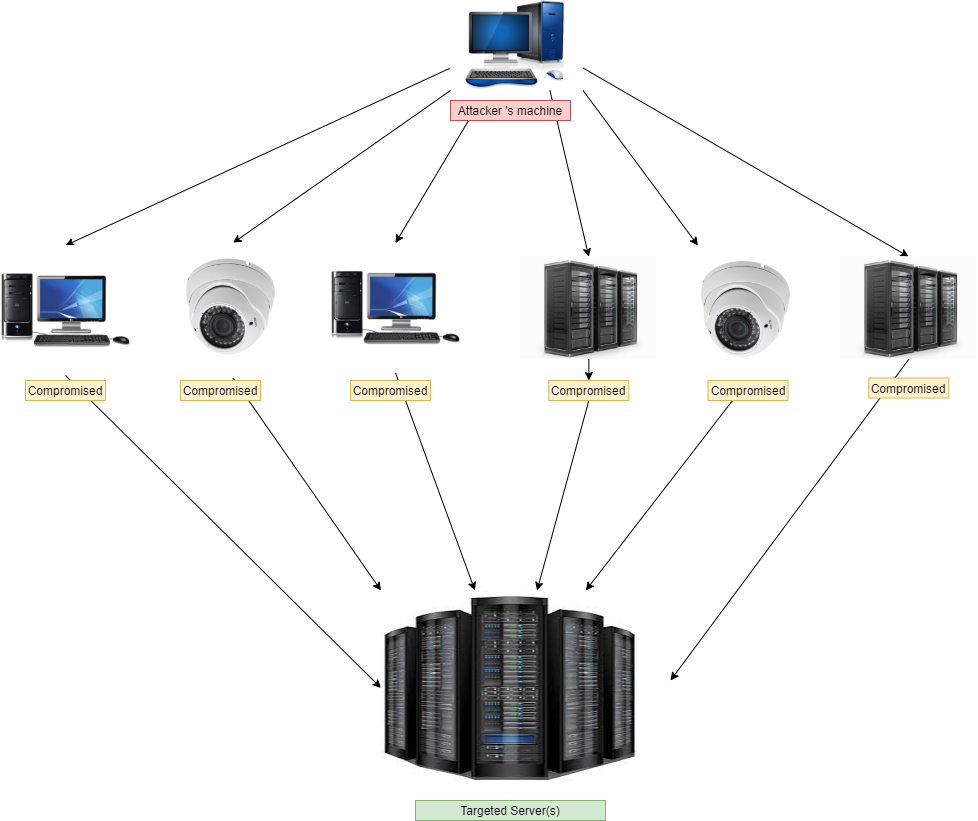
\includegraphics[width=\linewidth]{fig/ddos-model-example.png}
	\caption{Mô hình tấn công DDoS}
	\label{fig:ddos-model-example}
\end{figure}

\subsubsection{Các loại tấn công từ chối địch vụ phân tán thường gặp}

Nhìn chung, theo như các định nghĩa thì tấn công DDoS được thực hiện khi có rất nhiều thiết bị cùng lúc thực hiện tấn công DoS. Một số loại tấn công DDoS có thể liệt kê như sau:

Tấn công khuếch đại NTP \cite{2-imperva}, kẻ tấn công sẽ khai thác những máy chủ NTP công khai để làm quá tải nạn nhân với lưu lượng UDP. Loại tấn công này được xem là tấn công khuếch đại cưỡng đoạt bởi vì tỷ lệ phản hồi trong kịch bản này nằm ở đoạn 1:20 đến 1:200 và hơn thế nữa. Điều này có nghĩa là một kẻ tấn công nắm một lượng lớn máy chủ NTP có thể dễ dàng tạo nên tấn công DDoS với băng thông và lưu lượng cực lớn.

Tấn công ngập lụt HTTP \cite{2-imperva} là loại tấn công mà kẻ tấn công sẽ gửi những yêu cầu GET/POST HTTP trông giống các yêu cầu hợp lệ tới máy chủ web hoặc ứng dụng. Tấn công này không gửi các gói tin dị thường, kỹ thuật giả mạo hay phản chiếu, và yêu cầu ít băng thông hơn các kiểu tấn công khác để làm sập máy chủ nạn nhân. Đây là loại tấn công hiệu quả nhất khi nó buộc máy chủ hay ứng dụng phải sử dụng tối đa tài nguyên cho mỗi yêu cầu.

\subsubsection{Các đợt tấn công DoS/DDoS điển hình}

Theo \cite{6-wired} ghi nhận, vào năm 2016 thế giới chứng kiến một đợt tấn công DDoS ''lớn nhất từ trước đến nay'' nhắm vào Dyn – một đơn vị cung cấp dịch vụ DNS của Hoa Kỳ. Cuộc tấn công này là hệ quả từ việc bảo mật yếu kém từ các thiết bị IoT, cho phép kẻ tấn công chiếm quyền kiểm soát và cài đặt botnet. Đỉnh điểm của cuộc tấn công lên đến 1.2Tbps.

Theo \cite{7-wired}, vào năm 2018, Github – một công ty cung cấp dịch vụ lưu trữ mã nguồn lớn nhất thế giới có trụ sở tại Hoa Kỳ, đã trải qua một đợt tấn công DDoS lớn nhất lịch sử được ghi nhận, đỉnh điểm lên đến 1.35Tbps. Đây là hệ quả của việc bảo mật yếu kém của các máy chủ Memcached, giúp kẻ tấn công dễ dàng chiếm quyền kiểm soát và thực hiện cuộc tấn công khuếch đại. Kiểu tấn công này được ghi nhận tương tự như tấn công khuếch đại NTP nhưng với quy mô và sức mạnh lớn hơn gấp nhiều lần.

Bảng \ref{tab:large-ddos-attack-in-history} liệt kê một số cuộc tấn công DDoS quy mô lớn được ghi nhận cho đến nay.

\begin{table}[]
	\begin{tabular}{|l|l|l|l|}
		\hline
		\multicolumn{1}{|c|}{\textbf{\begin{tabular}[c]{@{}c@{}}Đơn vị \\ bị tấn công\end{tabular}}} &
		\multicolumn{1}{c|}{\textbf{Mô tả}} &
		\multicolumn{1}{c|}{\textbf{Thời gian}} &
		\multicolumn{1}{c|}{\textbf{\begin{tabular}[c]{@{}c@{}}Lưu lượng\\ cao nhất\end{tabular}}} \\ \hline
		Github &
		\begin{tabular}[c]{@{}l@{}}Dịch vụ lưu trữ dạng web cho \\ việc quản  lý mã nguồn\end{tabular} &
		2018 &
		1.35 Tbps \cite{7-wired} \\ \hline
		BBC & Đài truyền thông Anh     & 2015 & 602 Gbps \cite{8-bbc} \\ \hline
		Cloudflare &
		\begin{tabular}[c]{@{}l@{}}Một công ty Hoa Kỳ chuyên \\ cung cấp các dịch vụ an ninh\\ mạng\end{tabular} &
		2014 &
		$\sim$400 Gbps \cite{9-cnbc} \\ \hline
		Spamhaus &
		\begin{tabular}[c]{@{}l@{}}Một tổ chức phi lợi nhuận \\ chuyên theo dõi những kẻ \\ spam email và các hoạt động\\ liên quan đến spam\end{tabular} &
		2013 &
		$\sim$300Gbps \cite{10-cloudflare} \\ \hline
		Dyn & Nhà cung cấp dịch vụ DNS & 2016 & 1.2Tbps \cite{6-wired}  \\ \hline
	\end{tabular}
\caption{Một số cuộc tấn công DDoS quy mô lớn}
\label{tab:large-ddos-attack-in-history}
\end{table}

\section{Mạng định nghĩa bằng phần mềm (Software Defined Network)}

\subsection{Software defined network là gì}
\label{sec:sdn}

Khái niệm Software defined network (SDN) nguyên thủy được đặt ra để trình bày ý tưởng và làm việc với Openflow \cite{13-McKeown} tại đại học Standford (Standford, CA, USA).

Theo D.Kreutz và các cộng sự \cite{11-Kreutz}, như định  nghĩa ban đầu, SDN đề cập đến một kiến trúc mạng, mà ở đó trạng thái chuyển tiếp (forwarding state) trong plane dữ liệu (data plane) được quản lý bằng  một plane được điều khiển từ xa (remotely controlled plane) tách rời. Kiến trúc SDN được định nghĩa dụa trên 4 yếu tố.

\begin{itemize}
\item[--] Control plane và data plane được tách rời. Những tính năng điều khiển được di chuyển ra khỏi những thiết bị mạng, thì những thiết bị mạng này trở thành phần chuyển tiếp gói tin đơn giản.
\item[--] Quyết định chuyển tiếp được dựa trên luồng (flow), thay vì dựa trên đích đến. Một luồng được định nghĩa là một tập hợp các giá trị trường gói tin đóng vai trò là tiêu chí khớp (bộ lọc) và tập hợp hành động (chỉ dẫn). Trong bối cảnh SDN/Openflow, một luồng là một chuỗi những gói tin giữa một nguồn và một đích. Tất cả gói tin trong một luồng nhận những chính sách dịch vụ giống hệt nhau tại thiết bị chuyển tiếp. Sự trừu tượng của luồng cho phép thống nhất những loại hành động khác nhau của những thiết bị mạng, bao gồm các router, switch, firewall, middleboxes. Lập trình luồng cho phép sự linh hoạt chưa từng có, chỉ giới hạn ở khả năng của các flow-table được triển khai.
\item[--] Điều khiển logic được di chuyển ra khỏi các thực thể bên trong, được gọi là SDN controller hay Network operating system (NOS). NOS là nền tảng phần mềm được chạy trên công nghệ máy chủ và cung cấp những tài nguyên thiết yếu trừu tượng để tạo điều kiện cho việc lập trình các thiết bị chuyển tiếp dựa trên một chế độ mạng trừu tượng và tập trung logic. Mục đích của nó thì giống với hệ điều hành truyền thống.
\item[--] Mạng có thể lập trình được thông qua những ứng dụng phần mềm ở tầng đầu của NOS, mà ở đó tương tác với những thiết bị ở data plane. Đậy là đặc tính cơ bản của SDN được xem là giá trị chính của nó. 
\end{itemize}

Hình \ref{fig:sdn-infrastructure} thể hiện kiến trúc và sự trừu tượng cơ bản của SDN.

\begin{figure}[ht!]
	\centering
	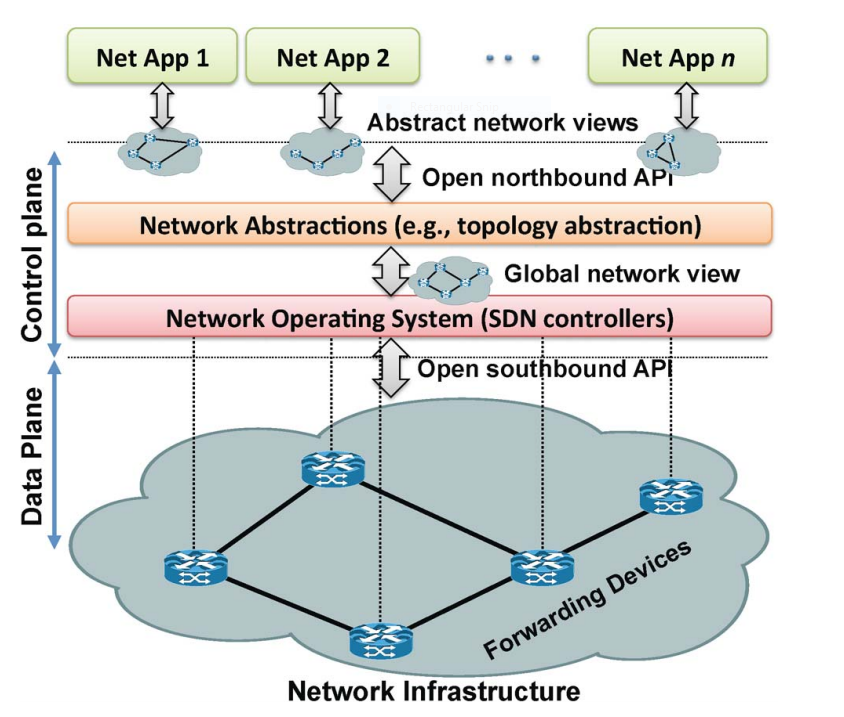
\includegraphics[width=0.75\linewidth]{fig/sdn-infrastructure.png}
	\caption{Kiến trúc của SDN \cite{11-Kreutz}}
	\label{fig:sdn-infrastructure}
\end{figure}

Openflow \cite{13-McKeown} được đề xuất để tiêu chuẩn giao tiếp giữa các switch và controller trong kiến trúc SDN \cite{14-Lara}. Các tác giả nhận định rằng, thật khó để cộng đồng nghiên cứu mạng có thể kiểm tra ý tưởng mới ở các phần cứng hiện tại. Việc này diễn ra bởi vì mã nguồn của phần mềm chạy trên các switch không thể được tùy chỉnh và các kiến trúc mạng thì luôn cố định, dẫn tới những ý tưởng mạng mới không thể được kiểm tra trên những cài đặt lưu lượng thực tế. Bằng việc xác định các đặc trưng thông thường trên những bảng luồng trong các switch Ethernet, các tác giả đã cung cấp cách điều khiển switch mà không cần quan tâm đến mã nguồn trên các thiết bị đó.
	
Openflow lần đầu được triển khai trong khuôn viên mạng đại học \cite{13-McKeown}. Ngày nay, có ít nhất 9 trường đại học ở Hoa Kỳ triển khai công nghệ này. Mục đích của Openflow là cung cấp nền tảng mà có thể cho phép các nhà nghiên cứu chạy thử nghiệm những sản phẩm mạng. Tuy nhiên, SDN và Openflow được gắn kết như chiến lược để gia tăng chức năng chức năng của mạng trong khi giảm thiểu chi phí và độ phức tạp phần cứng. Openflow Networking Foundation (ONF) được thành lập vào năm 2011 bởi Deutsche Telekom, Facebook, Google, Microsoft, Verizon và Yahoo để khuyến khích áp dụng mạng dựa trên SDN và Openflow. Hiện tại, ONF có hơn 95 thành viên bào gồm thành viên sáng lập.

Bảng \ref{tab:ofswitch-company} liệt kê một số công ty cung cấp Openflow switch trên thị trường.

\begin{table}[ht!]
	\centering
	\begin{tabular}{|l|l|}
		\hline
		\multicolumn{1}{|c|}{\textbf{Switch company}} &
		\multicolumn{1}{c|}{\textbf{Series}} \\ \hline
		Arista &
		\begin{tabular}[c]{@{}l@{}}Arista   extensible modular operating system (EOS),\\  Arista 7124FX application switch\end{tabular} \\ \hline
		Ciena          & Ciena   Coredirector running firmware version 6.1.1 \\ \hline
		Cisco          & Cisco   cat6k, catalyst 3750, 6500 series           \\ \hline
		HP &
		\begin{tabular}[c]{@{}l@{}}HP   procurve series- 5400 zl, 8200 zl, 6200 yl, \\ 3500 yl, 6600\end{tabular} \\ \hline
		NEC            & NEC   IP8800                                        \\ \hline
		Open   vSwitch & Software   switch.                                  \\ \hline
	\end{tabular}
\caption{Một số công ty cung cấp OpenFlow Switch}
\label{tab:ofswitch-company}
\end{table}

Trong khuôn khổ của khóa luận này, Open vSwitch sẽ được sử dụng là một thành phần chính trong triển khai SDN, được giới thiệu chi tiết trong mục \ref{sec:openvswtich}.

\subsection{Open vSwitch}
\label{sec:openvswtich}

\subsubsection{Open vSwitch (OVS) là gì?}

Open vSwitch là switch phần mềm đa lớp bản quyền mã nguồn mở Apache 2. Mục tiêu là để triển khai một nền tảng sản phẩm switch chất lượng hỗ trợ các giao diện quản lý tiêu chuẩn và mở ra chức năng chuyển tiếp để mở rộng và kiểm soát bằng lập trình.

OVS rất thích hợp với chức năng như một switch ảo trong môi trường máy ảo. Ngoài việc hiển thị các giao diện điều khiển và hiển thị tiêu chuẩn cho lớp mạng ảo, nó còn được thiết kế để hỗ trợ phân phối trên nhiều máy chủ vật lý. OVS hỗ trợ nhiều công nghệ ảo hóa dựa trên Linux bao gồm Xen/XenServer, KVM và Virtualbox. Hình \ref{fig:ovs} thể hiện kiến trúc tổng quan và chức năng của OVS.

\begin{figure}[ht!]
	\centering
	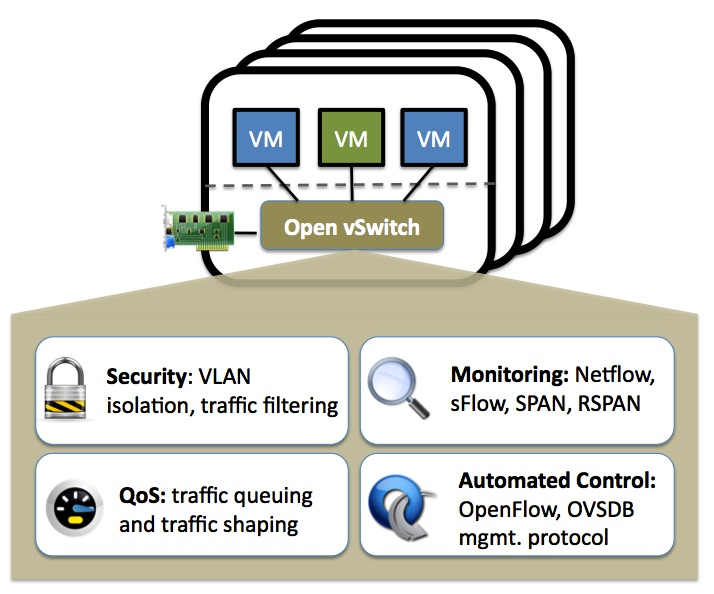
\includegraphics[width=0.5\linewidth]{fig/ovs.png}
	\caption{Kiến trúc tổng quan và chức năng của OVS \cite{16-openvswitch}}
	\label{fig:ovs}
\end{figure}

\subsection{Vai trò của SDN controller}

\subsubsection{Tổng quan}

Dựa theo các định nghĩa đã được đưa ra, SDN controller là hệ quả của việc tách rời Data plane và Control plane trong hệ thống mạng. Nó có vai trò trung tập điều khiển tất cả các hoạt động của mạng bằng việc điều khiển các switch và router thông qua flow-table. Nói cách khác, SDN controller như là bộ não của toàn bộ hệ thống. Để có thể giao tiếp với các thiết bị mạng, SDN controller sử dụng một giao thức chuẩn là Openflow như đã đề cập tại mục \ref{sec:sdn}. Hình \ref{fig:sdn-infrastructure} cho thấy, SDN controller như một cầu nối giữa các thiết bị mạng và các ứng dụng ở phần trên.

Hiện nay có rất nhiều phần mềm hay framework hỗ trợ việc lập trình SDN controller như OpenDaylight, ONOS, POX, Ryu, vv. Trong khuôn khổ của dự án này, Ryu framework được sử dụng như thành phần chính để lập trình và thực thi SDN controller, được giới thiệu chi tiết bên dưới mục "Framework RYU".

\subsubsection{Framework RYU}
\label{sec:ryu}

Theo \cite{17-Asadollahi}, Ryu Controller là một dự án mã nguồn mở dưới giấy phép của Apache 2.0, được viết hoàn toàn dựa trên Python, được hỗ trợ và triển khai bởi trung tâm dữ liệu đám mây NTT. Phần mã nguồn chính có thể được tìm thấy trên Github, được cung cấp và hỗ trợ bởi Open Ryu Community. Nó hỗ trợ quản trị mạng NETCONF và OF-config, còn được biết đến là Openflow. Ryu đã được kiểm định với OVS switch, Hewlett Packard, IBM và NEC. Hiện tại nó đang hỗ trợ đến phiên bản Openflow 1.5.

Cũng như các SDN controller khác, Ryu cũng tạo ra các gói tin Openflow, quản lý các sự kiện liên quan tới những gói tin đến và đi. Nó còn có một danh sách phong phú các thư viện hỗ trợ xử lý hoạt động của các gói tin. Về hỗ trợ các giao thức southbound, 	Ryu hợp tác với các giao thức như Xflow (Netflow và Sflow), OF-config, NETCONF, Open vSwitch Database Protocol, vv, VLAN và GRE cũng được hỗ trợ bởi những thư viện gói tin của Ryu.

\section{Học máy (Machine Learning)}

\subsection{Học máy là gì?}

Theo A.Dey \cite{18-Dey} trích dẫn, học máy được dùng để dạy máy móc cách để xử lý dữ liệu hiệu quả hơn. Đôi khi, sau khi xem xét dữ liệu, chúng ta không thể giải thích được mẫu hoặc trích xuất thông tin từ chúng. Trong trường hợp này, chúng ta có thể áp dụng học máy. Với vô số tập dữ liệu (dataset) hiện có, nhu cầu về học máy ngày càng tăng. Rất nhiều ngành công nghiệp từ dược liệu cho đến quân sự đều ứng dụng học máy để trích xuất thông tin liên quan từ dữ liệu. Công việc chính của học máy là học từ dữ liệu. Có rất nhiều nghiên cứu đã tìm ra được cách để máy móc có thể học từ chính chúng \cite{19-Welling}, \cite{20-Bowles}. Có rất nhiều nhà toán học và lập trình viên ứng dụng nhiều hướng tiếp cận để tìm ra giải pháp cho vấn đề này. Một vài trong số chúng được biểu thị trong hình \ref{fig:ml-algo}.

\begin{figure}[ht!]
	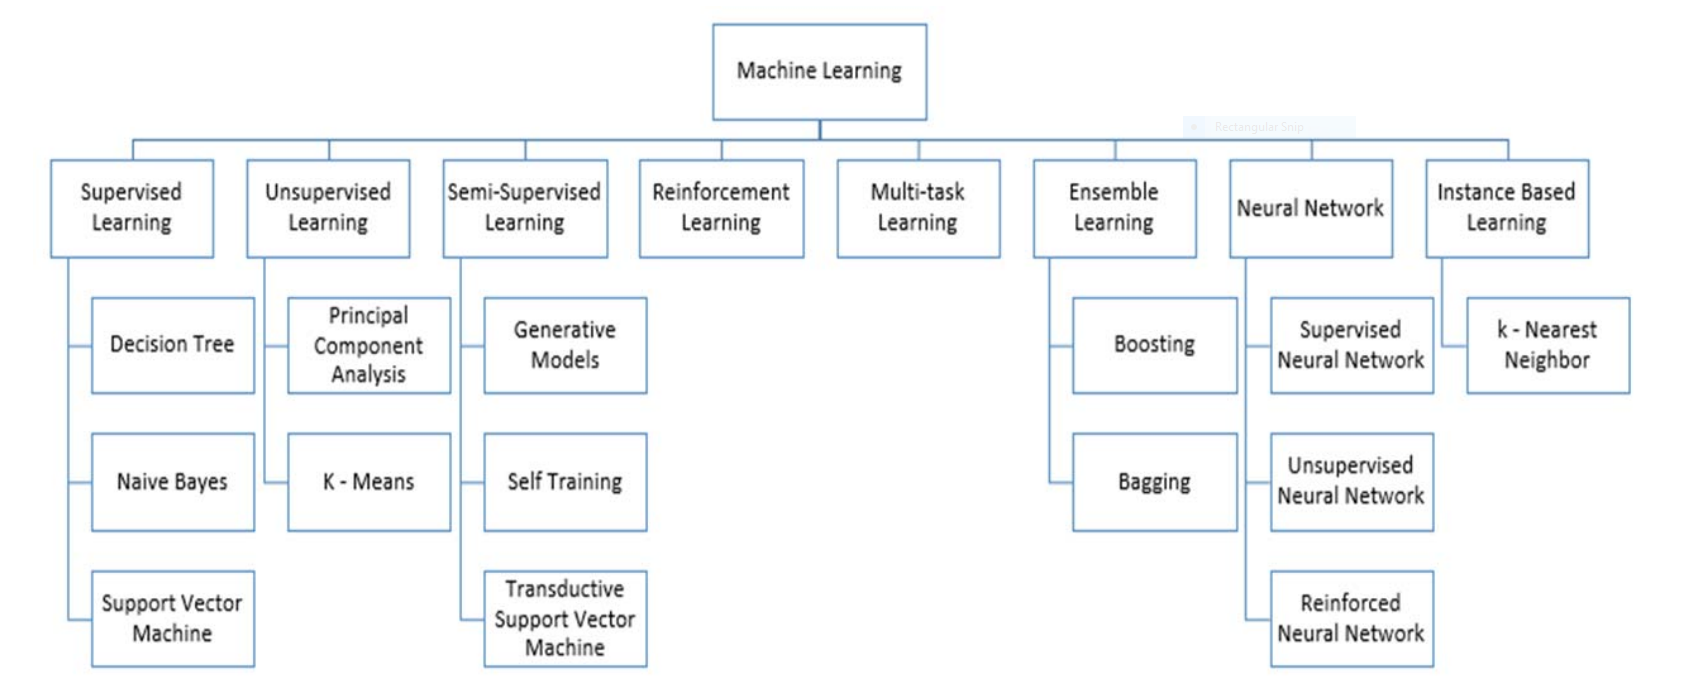
\includegraphics[width=\linewidth]{fig/ml-algo.png}
	\caption{Một số giải thuật học máy \cite{18-Dey}}
	\label{fig:ml-algo}
\end{figure}

\subsection{Mô hình học máy}

Theo như hình \ref{fig:ml-algo}, học máy được phân ra thành rất nhiều loại như Supervised learning (học có giám sát), Unsupervised learning (học không có giám sát), Semi-supervised learning (học bán giám sát), vv. Trong khuôn khổ của khóa luận này, tôi chỉ giới thiệu một số giải thuật là Support Vector Machine, Naïve Bayes, Decision Tree và Random Forest trong nhóm Học có giám sát, vì đây là các giải thuật được tôi áp dụng vào khóa luận.

\subsubsection{Học có giám sát}

Các thuật toán học có giám sát là những thuật toán cần sự hỗ trợ từ bên trong. Đầu vào của dữ liệu cần chia ra thành tập huấn luyện (train set) và tập kiểm tra (test set). Train set có giá trị đầu ra, thứ cần được dự đoán hoặc phân loại. Tất cả các thuật toán đều được học hình mẫu từ train set và sau đó vận dụng chúng vào test set để đánh giá \cite{21-Kotsiantis}. Giải thuật học có giám sát được biểu thị trong hình \ref{fig:supervised-ml}.

\begin{figure}[ht!]
	\centering
	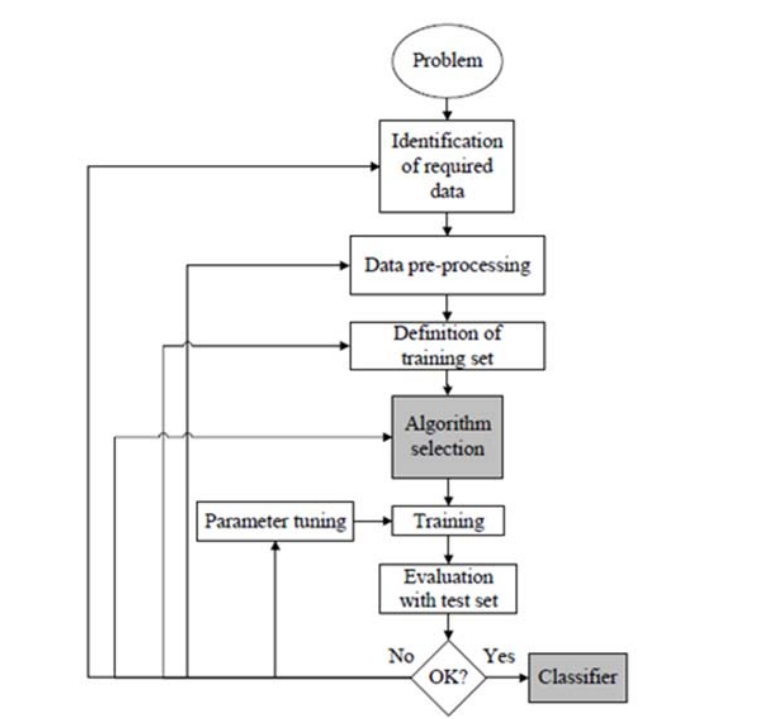
\includegraphics[width=0.6\linewidth]{fig/supervised-ml.png}
	\caption{Giải thuật học máy có giám sát \cite{18-Dey}}
	\label{fig:supervised-ml}
\end{figure} 

\subsubsection{Support Vector Machine}

Một kỹ thuật học máy state-of-the-art được sử dụng rộng rãi là Support Vector Machine (SVM). Nó được dùng chủ yếu trong bài toán phân loại. SVM hoạt động dựa trên nguyên lý của tính toán biên. Các biên được vẽ sao cho khoảng cách giữa biên đến các lớp là lớp nhất và vì vậy giảm thiểu sai số phân loại. Mô tả SVM được biểu thị trong hình \ref{fig:svm-overview}.

\begin{figure}[ht!]
	\centering
	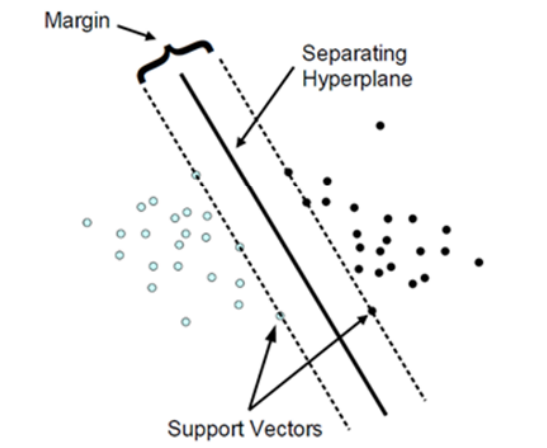
\includegraphics[width=0.5\linewidth]{fig/svm-overview.png}
	\caption{Mô tả mô hình SVM \cite{18-Dey}}
	\label{fig:svm-overview}
\end{figure}

\subsubsection{Naïve Bayes}

Naïve Bayes được áp dụng chủ yếu trong lĩnh vực phân loại văn bản. Nó được sử dụng chủ yếu cho việc phân cụm và phân lớp. Kiến trúc cơ bản của Naïve Bayes phụ thuộc vào xác suất có điều kiện. Nó tạo ra cây dựa trên xác suất xảy ra của chúng. Những cây này được gọi là Bayesian Network. Ví dụ cho Bayesian Network được biểu thị trong hình \ref{fig:naive-bayes-example}.

\begin{figure}[ht!]
	\centering
	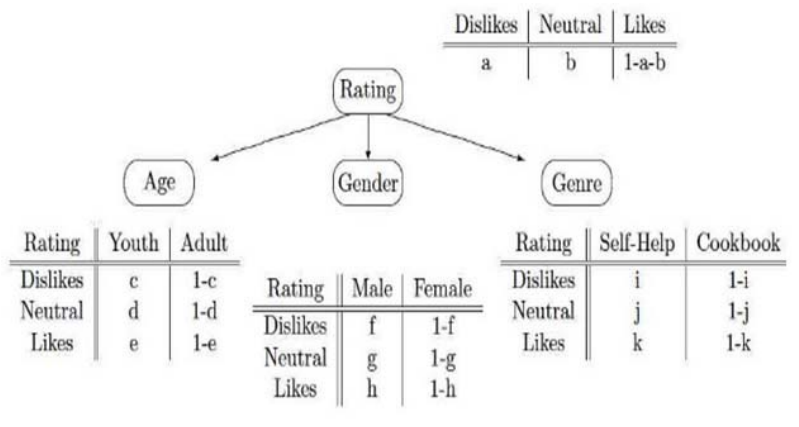
\includegraphics[width=0.75\linewidth]{fig/naive-bayes-example.png}
	\caption{Một ví dụ về Bayesian Network \cite{18-Dey}}
	\label{fig:naive-bayes-example}
\end{figure}

\subsubsection{Decision Tree}

Decision trees (những cây quyết định) là những loại cây gom nhóm các thuộc tính dựa trên giá trị của chúng. Decision tree được sử dụng chủ yếu cho việc phân lớp. Môi cây chứa nhiều nút và nhiều nhánh. Mỗi nút biểu diễn cho những thuộc tính trong một nhóm để phân lớp và mỗi nhánh biểu diễn một giá trị  mà nút đó có thể lấy. Một ví dụ cho Decision tree trong hình \ref{fig:decision-tree-example}.

\begin{figure}[ht!]
	\centering
	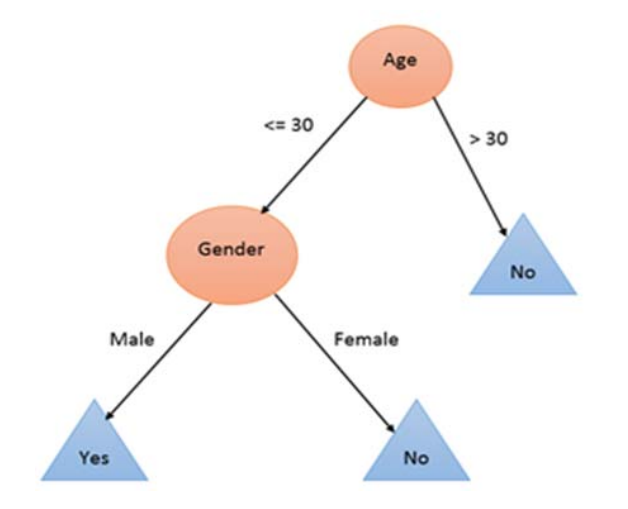
\includegraphics[width=0.6\linewidth]{fig/decision-tree-example.png}
	\caption{Một ví dụ cho Decision Tree}
	\label{fig:decision-tree-example}
\end{figure}

\subsubsection{Random Forest}

Random forest được đề xuất lần đầu bởi Leo Breiman từ đại học California vào năm 2001. Nó kết hợp nhiều máy phân lớp đơn giản (các cây quyết định) độc lập với nhau. Kết quả của phân lớp của một mẫu được đưa ra bởi nhiều cây quyết đinh, kết quả cuối cùng sẽ được bình chọn dựa trên kết quả của các cây quyết định này \cite{70-Parmar}.Toàn bộ quy trình phân lớp dựa trên Random Forest được biểu diễn như trong hình \ref{fig:random-forest-example}.

\begin{figure}[ht!]
	\centering
	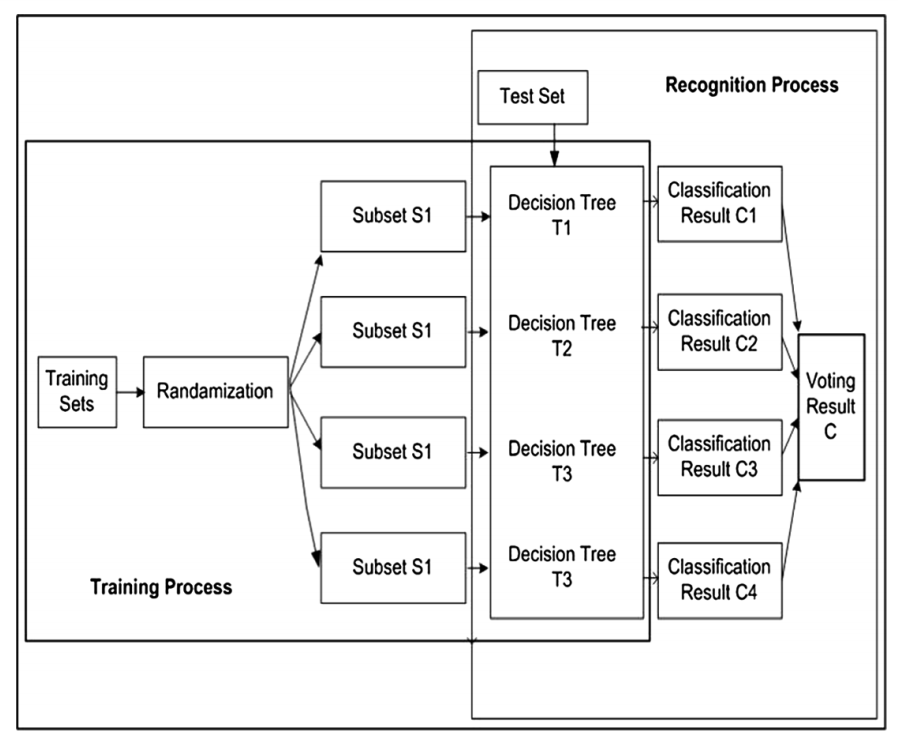
\includegraphics[width=0.75\linewidth]{fig/random-forest-example.png}
	\caption{Quá trình máy phân lớp  Random  forest}
	\label{fig:random-forest-example}
\end{figure}

\subsection{Thư viện scikit-learn}

Scikit-learn là thư viện cung cấp sẵn một lượng lớn các giải thuật học máy có giám sát và không có giám sát thông qua giao diện lập trình Python.

Đây là thư viện mã nguồn mở, giấy phép cấp bởi BSD và được phân phối sẵn trên nhiều nền tảng hệ điều hành Linux.

Scikit-learn được phát triển lần đầu bởi David Cournapeau như một dự án mùa hè tại Google năm 2007. Sau đó Matthieu Brucher tham gia dự án và bắt đầu sử dụng thư viện này như một phần trong luận văn của anh ấy. Năm 2010, INRIA tham gia và lần đầu xuất bản phiên bản đầu tiên (v0.1 beta) vào cuối tháng 1 năm 2010. Dự án hiện tại có trên 30 nhà phát triển đóng góp và được tài trợ trả phí từ INRIA, Google, Tinyclues và Python software foundation.

\section{Học sâu (Deep learning)}

\subsection{Học sâu là gì}

Theo X. Du và các cộng sự \cite{25-Du}, học sâu trong quá khứ được phát triển từ mạng nơ-ron nhân tạo, và bây giờ nó trở nhành một lĩnh vực thịnh hành của học máy. Nghiên cứu về mạng nơ-ron nhân tạo bắt đầu từ những năm 1940. McCulloch và các cộng sự \cite{26-McCulloch} đã đề xuất mô hình McCulloch-Pitts với việc phân tích và tổng hợp những nét đặc trưng của mạng nơ-ron. Khái niệm học sâu được đưa ra lần đầu vào năm 2006. Sau đó, học sâu vẫn tiếp tục được phát triển mạnh. Hiện tại, có rất nhiều tên tuổi nổi bật như Geoffrey Hinton, Yoshua Bengio, Yann LeCun và Andrew Ng. Họ là những người dẫn đầu về hướng nghiên cứu học sâu. 

Một số doanh nghiệp, ví dụ như Google và Facebook đã có rất nhiều nghiên cứu đạt được thành công và áp dụng trong nhiều lĩnh vực khác nhau. Đơn cử như Google’s AlphaGo đã đánh bại Lee Sedol – kỳ thủ cờ vây chuyên nghiệp người Hàn Quốc, cho thấy khả năng học rất mạnh của học sâu. Hơn nữa, Google’s DeepDream và một phần mềm tuyệt vời, thứ không chỉ phân loại hình ảnh mà còn tạo ra được những hình vẽ nhân tạo kỳ lạ dựa trên chính kiến thức của nó. Bên cạnh đó, Facebook với DeepText – một kỹ thuật hiểu văn bản dựa trên học sâu, có thể phân loại một lượng dữ liệu khổng lồ, cung cấp dịch vụ phản hồi sau khi xác định những đoạn trò chuyện của người dùng và xóa các đoạn thư spam.

\subsection{Mô hình học sâu}

\subsubsection{Khái niệm và phân loại}

\textit{Mạng nơ-ron - Neural Network}

Mạng nơ-ron (hay mạng nơ-ron nhân tạo hay ANN) được kế thừa từ khái niệm nơ-rơn sinh học. Một nơ-rơn như một cấu trúc trong não. Để hiểu được mạng nơ-ron, người ta cần phải hiểu cách hoạt động của nơ-ron. Một nơ-ron bao gồm 4 phần chính là dendrites, nucleus, soma và axon (Hình \ref{fig:bio-nn}). 

\begin{figure}[ht!]
	\centering
	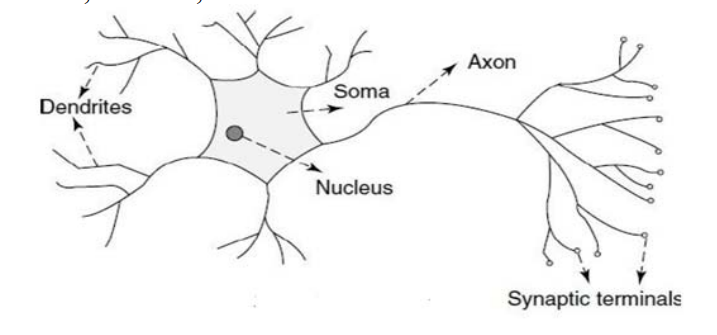
\includegraphics[width=0.75\linewidth]{fig/bio-nn.png}
	\caption{Mạng nơ-ron sinh học}
	\label{fig:bio-nn}
\end{figure}

Các dendrite nhận tín hiệu điện. Soma xử lý tín hiệu điện. Đầu ra của quá trình được vận chuyển bởi axon đển cổng dendrite nơi mà đầu ra được gửi tiếp đến nơ-ron tiếp theo. Necleus là trái tim của nơ-ron. Kết nối bên trong nơ-ron được gọi là mạng nơ-ron nơi mà các xung điện di chuyển khắp não.

Một mạng nơ-ron nhân tạo cũng hoạt động tương tự. Nó hoạt động với 3 tầng. Tầng đầu vào (input) nhận dữ liệu đầu vào (tương tự dendrite). Những tầng ẩn thì xử lý dữ liệu (tương tự soma và axon). Cuối cùng, tầng đầu ra (output) gửi kết quả đã được tính toán (tương tự dendrite terminal). Cấu trúc ví dụ của mạng nơ-ron nhân tạo được biểu thị trong hình \ref{fig:cs-nn}

\begin{figure}[h]
	\centering
	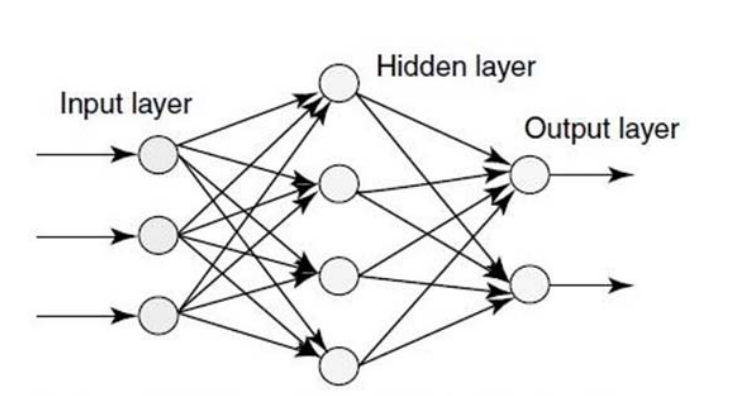
\includegraphics[width=0.75\linewidth]{fig/cs-nn.png}
	\caption{Mạng nơ-ron nhân tạo}
	\label{fig:cs-nn}
\end{figure}

Theo Shrestha và các cộng sự \cite{62-Shrestha}, mạng nơ-ron nhân có thể được chia ra thành các loại sau:

\begin{itemize}
	\item[--] Mạng nơ-ron suy luận tiến (Feedforward Neural Network)
	\item[--] Mạng nơ-ron hồi quy (Recurrent Neural Network (RNN))
	\item[--] Mạng chức năng cơ sở xuyên tâm (Radial Basis Function Neural Network)
	\item[--] Mạng nơ-ron ánh xạ đặc trưng tự tổ chức (Kohonen Self Organizing Neural Network)
	\item[--] Mạng nơ-ron mô-đun
\end{itemize}

Trong mạng nơ-ron suy luận tiến, những luồng thông tin chỉ đi theo 1 chiều từ  lớp đầu vào đến lớp đầu ra (đi qua các nút ẩn nếu có). Chúng không có tạo thành bất cứ vòng lặp hay luận lùi. Hình \ref{fig:feed-forward-nn} biểu thị một triển khai cụ thể của mạng nơ-ron suy tiến đa lớp với các giá trị và các hàm được tính toán theo chiều tiến. Z là tổng trọng số của các đầu vào và y biểu diễn một hàm không tuyến tính f của Z ở mỗi lớp. W biểu diễn cho những trọng số giữa 2 đơn vị trong những lớp liền kề biểu diễn bởi ký tự chỉ số dưới và b biểu diễn cho giá trị sai khác của đơn vị.

\begin{figure}[ht!]
	\centering
	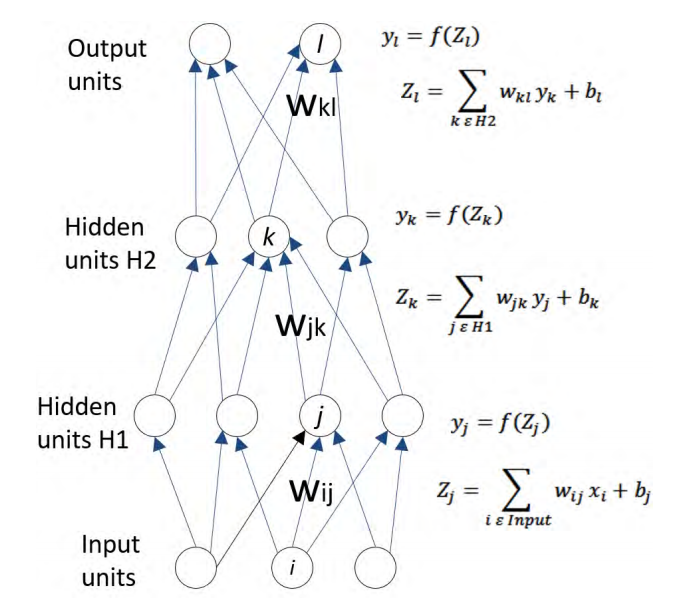
\includegraphics[width=0.6\linewidth]{fig/feed-forward-nn.png}
	\caption{Mạng nơ-ron suy luận tiến \cite{62-Shrestha}}
	\label{fig:feed-forward-nn}
\end{figure}

Không giống như mạng nơ-ron suy luận tiến, việc xử lý đơn vị trong RNN có vòng lặp. Đầu ra của lớp trước trở thành đầu vào cho lớp sau, thứ đơn thuần chỉ là 1 lớp trong mạng, vì vậy chính đầu ra của lớp cũng trở thành chính đầu vào của nó biểu diễn một vòng tự lặp. Điều này cho phép mạng có ký tức về những trạng thái trước đó và sử dụng nó để ảnh hướng lên đầu ra hiện tại. Một lợi thế lớn của đặc điểm này so với mạng nơ-ron suy tiến là RNN có thể nhận chuỗi đầu vào và trả về chuỗi đầu ra, vì vậy nó rất hữu ích cho các ứng dụng cần xử lý đầu vào dạng chuỗi theo thời gian như nhận diện giọng nói, phân loại từng khung hình của video, vv. Hình \ref{fig:rnn} biểu diễn một triển khai của RNN. Trong đó \(x^t\) biểu diễn cho đầu vào tại thời điểm t. U, V và W là các  tham số học được chia sẽ bởi tất cả bước. \(O_t\) là đầu ra tại thời điểm t. \(S_t\) biểu diễn trạng thái tại thời điểm t.

\begin{figure}[ht!]
	\centering
	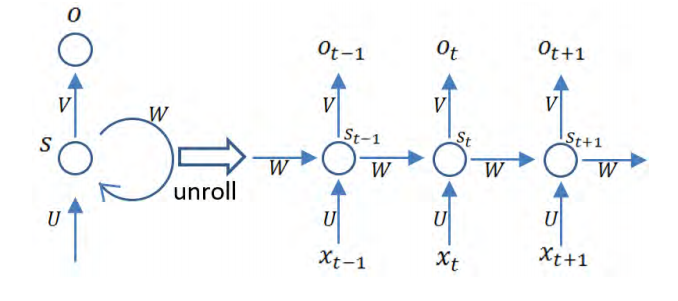
\includegraphics[width=0.75\linewidth]{fig/rnn.png}
	\caption{Mạng nơ-ron hồi quy \cite{62-Shrestha}}
	\label{fig:rnn}
\end{figure}

Mạng chức năng cơ sở xuyên tâm được dùng trong phân lớp, xấp xỉ hàm, những vấn đề dự doán theo thời gian, vv.

Mạng nơ-ron ánh xạ đặc trưng tự tổ chức có thể tự tổ chức mô hình mạng dựa trên dữ liệu đầu vào bằng việc học không giám sát.

Mạng nơ-ron mô-đun tách một mạng lớn thành các mô-đun mạng nơ-ron nhỏ độc lập. Những mạng nhỏ hơn giải quyết công việc khác nhau và sau đó kết hợp tại một điểm đầu ra của toàn bộ mạng.

\subsubsection{Một số khái niệm về các hàm huấn luyện}

\textit{Hàm kích hoạt (Activation function)}

Theo \cite{63-Nwankpa}, những hàm kích hoạt là những hàm dùng trong mạng nơ-ron để tính toán tổng trọng số của đầu vào và những sai khác (bias), thứ quyết định nơ-ron được thực hiện hay không. Nó thao tác với dữ liệu thông qua quá trình gradient thường là giảm gradient và sau đó sinh ra kết quả cho mạng nơ-ron mà có chứa tham số cho dữ liệu. Hàm kích hoạt có thể tuyến tính hoặc không tuyến tính tùy thuộc vào hàm mà nó  biểu diễn và được dùng để điều khiển đầu ra cho mạng nơ-ron.  Một số hàm kích hoạt biểu diễn trong công thức (\ref{eq:softmax}) và (\ref{eq:relu}).

\begin{itemize}
	\item[--] Hàm  Softmax: 
		\begin{gather}
		\label{eq:softmax}
			f(x) = \frac{exp(x_i)}{\sum_{j} exp(x_j)}
		\end{gather} 
	\item[--] Hàm ReLU: 
		\begin{gather}
		\label{eq:relu}
			f(x) = max(0, x)
		\end{gather}
\end{itemize}

\textit{Hàm mất mát (Loss function)}

Hàm mất mát đơn giản là hàm dùng để đánh giá mức độ tốt của mô hình giải thuật. Nếu dự đoán tốt hàm sẽ cho ra giá trị thấp, ngược lại hàm cho ra giá trị cao. Công thức của hàm mất mát Categorical Cross Entroy biểu diễn ở công thức (\ref{eq:loss_cce}).

\begin{gather}
\label{eq:loss_cce}
	Loss = - \sum_{i=1}^{output size} y_i \cdot log \hat{y}_i
\end{gather}

\subsection{Thư viện Tensorflow và Keras}

Tensorflow hiện nay là bộ thư viện học sâu nổi tiếng nhất được phát triển bởi Google. Nó lần đầu tiên được công bố vào cuối năm 2015, trong khi phiên bản ổn định đầu tiên ra đời năm 2017. Tensorflow là thư viện mã nguồn mở dưới giấy phép của Apache Opensource. Người ta có thể sử dụng, tinh chỉnh, và phân phối lại phiên bản tinh chỉnh mà không cần phải trả một khoản nào cho Google.

Keras là một thư viện mã nguồn dưới bản quyền MIT. Keras cung cấp một API ở mức cao, nằm trên các thư viện học sâu như Tensorflow, Theano, CNTK với mục tiêu giúp đơn giản hóa việc tiếp cận nền tảng học sâu. Keras được xây dựng với mục đích cung cấp giao diện thân thiện, mô-đun hóa, và dễ mở rộng.

Năm 2017, Google’s Tensorflow team quyết định hỗ trợ Keras nằm trực tiếp trong phần nhân của thư viện tensorflow.


\chapter{Các công trình liên quan}
\label{chap:review}
Trong chương này, chúng tôi sẽ tiến hành tìm hiểu, khảo sát các công trình liên quan đến chủ đề của khóa luận.


\section{Phát hiện tấn công DDoS với phương pháp thống kê}
\label{stat-method}

R. Doriguzzi-Corin và các cộng sự \cite{27-Corin} cho rằng, đo lường các đặc tính thống kê của các thuộc tính lưu lượng mạng là phương pháp thông dụng để phát hiện tấn công DDoS, thường liên quan đến việc quan sát sự biến đổi entropy của trường header trong các gói tin. Bằng định nghĩa này, entropy là đo lường của sự đa dạng hay sự ngẫu nhiên trong tập dữ liệu. Phương thức phát hiện tấn công DDoS dựa trên entropy đã được đưa ra ở các nghiên cứu học thuật vào những năm 2000, dựa trên giả sử rằng, trong suốt quá trình tấn công DDoS băng thông, tính ngẫu nhiên của đặc trưng lưu lượng biến đổi đột ngột. Lý do là đặc trưng của các cuộc tấn công DDoS băng thông thường có một số lượng lớn kẻ tấn công, thông thường là các thiết bị bị xâm nhập gửi một lượng lớn yêu cầu đến nạn nhân. Do đó, các cuộc tấn công này tường gây ra sự sụt giảm trong việc phân phối một số thuộc tính lưu lượng truy cập, chẳng hạn như địa chỉ IP đích, hoặc sự gia tăng trong việc phân phối các thuộc tính khác, ví dụ như địa chỉ IP nguồn. Cách xác định tấn công DDoS thường phụ thuộc vào giá trị trung bình của ngưỡng của các chỉ số phân phối này.

Feinstein và các cộng sự \cite{29-Feinstein} đã trình bày kỹ thuật phát hiện DDoS dựa trên việc tính toán entropy của IP nguồn và phân phối Chi bình phương. Tác giả đã quan sát sự thay đổi trong entropy IP nguồn và thống kê Chi bình thương thông qua sự biến động của các lưu lượng hợp lệ thì nhỏ, so với độ lệch do lưu lượng tấn công gây ra. Tương tự vậy, P. Bojovic và các cộng sự \cite{30-Bojovic} đã kết hợp entropy với đặc tính lưu lượng băng thông để phát hiện tấn công DDoS băng thông.

Một hạn chế thường thấy ở kỹ thuật dựa trên entropy là sự bắt buộc chọn lấy một ngưỡng phát hiện chính xác. Các hệ thống mạng khác nhau sẽ có độ lệch về băng thông khác nhau, dẫn đến thách thức trong việc áp dụng một ngưỡng chính xác sao cho giảm tối thiểu các tỷ lệ nhận diện sai trong các kịch bản tấn công khác nhau. Một giải pháp được đề xuất bởi Kumar và các cộng sự \cite{32-Kumar} là gán linh động giá trị ngưỡng để có thể tự động thích nghi với lưu lượng mạng biến động thông thường. 


\section{Phát hiện DDoS với phương pháp học máy và học sâu}

\subsection{Một số dataset được sử dụng hiện nay}

Hiện nay có rất nhiều dataset dành cho lĩnh vực an toàn thông tin ra đời, trong đó, phần lớn đề cập đến vấn đề phát hiện và phòng thủ trước tấn công DoS/DDoS. M. Ring và các cộng sự \cite{33-Ring} đã có một khảo sát chi tiết các dataset liên quan đến an toàn thông tin, trong phần này tôi chỉ trích xuất ra các dataset liên quan đến tấn công DoS/DDoS.

Booters \cite{34-Santanna}. Booters là dịch vụ tấn công từ chối dịch vụ được sự dụng bởi các tin tặc. Santanna và các cộng sự \cite{34-Santanna} đã công bố dataset sử dụng 9 loại tấn công của Booters nhắm vào các máy tính trong mạng lưới của họ. Kết quả được ghi lại dưới dạng gói tin có lên tới 250GB lưu lượng mạng. Từng gói tin riêng lẻ thì không được dán nhãn, tuy nhiên các loại tấn công khác nhau được tách ra các tệp khác nhau. Dataset được công khai tuy nhiên tên của các loại tấn công bị ẩn đi do vấn đề về quyền riêng tư.

ISCX 2012 \cite{35-Shiravi}, được tạo ra vào năm 2012 bởi Canadian Institute for Cybersecurity (CIC) bằng việc bắt các gói tin trong môi trường mạng mô phỏng trong vòng 1 tuần. Tác giả sử dụng các phương pháp động để tạo ra dataset với các lưu lượng bình thường cũng như lưu lượng độc hại. Tác giả chia thành 2 phiên bản. Phiên bản alpha định nghĩa các kịch bản tấn công, phiên bản beta định nghĩa các kịch bản của người dùng thông thường bao gồm gửi email, lướt web, vv. Dựa vào phương pháp này, tác giả đã tạo ra dataset khá hoàn thiện, trong đó có các loại tấn công phổ biến mà bao gồm cả tấn công DoS và DDoS.

CIC-IDS-2017 \cite{36-Sharafaldin} và CSE-CIC-IDS-2018 \cite{36a-ids2018} đây là hai dataset cũng được thực hiện bởi CIC. Trong đó, CIC-IDS-2017 được công bố vào năm 2017, tác giả sử dụng các kỹ thuật tương tự như khi xây dựng dataset ISCX 2012. Tuy nhiên với phiên bản mới này, tác giả đã bổ sung nhiều loại tấn công hơn, chi tiết hơn về cách dán nhãn tấn công cũng như giới thiệu phần mềm phân tích lưu lượng mạng CICFlowMeter \cite{37-cicflowmeter}. Với kết quả của phần mềm này, các nhà nghiên cứu có thể dễ dàng áp dụng các phương pháp học máy và học sâu mà không cần phải tiển xử lý hàng trăm GB thông tin các gói tin. Hơn nữa, năm 2018, tác giả đã cho ra đời dataset CSE-CIC-IDS-2018 (gọi tắt là CICIDS2018), với việc kết hợp với AWS cloud service, để có thể tạo ra một mạng mô phỏng phức tạp sát với mạng lưới thực tế. Từ đó, tác giả áp dụng nhiều kịch bản tấn công làm cho dataset này trở thành dataset đầy đủ và tốt nhất hiện nay.

DARPA \cite{39-Lippmann}. DARPA là dataset được dùng rộng rãi trong phát hiện xâm nhập mạng, được tạo bởi MIT Lincoln Lab trong mạng mô phỏng. Dataset chứa nhiều loại tấn công như DoS, buffer overflow, port scan, rootkits.

KDD CUP 99 \cite{38-Stolfo} dựa trên DARPA dataset và trở thành dataset được sử dụng rộng rãi. Dataset này không chứa đựng thông tin gói tin hay thông tin flow, mà đơn giản là chỉ chứa các chỉ mục. Ở đó bao gồm các thuộc tính của các kết nối TCP, các thuộc tính cấp cao như số lần đăng nhập sai, và hơn 20 thuộc tính khác nữa.

NSL-KDD \cite{40-Tavallaee}. NSL-KDD là phiên bản nâng cấp của KDD CUP 99 với việc loại bỏ phần lớn các thông tin dư thừa. Dataset này có 150,000 điểm dữ liệu được chia ra thành tập huấn luyện và tập kiểm tra.

\subsection{Một số công trình sử dụng phương pháp học máy}

Có nhiều công trình nghiên cứu sử dụng học máy vào việc phát hiện tấn công DoS/DDoS.
He và các cộng sự \cite{41-He} đã sử dụng 9 loại giải thuật học máy gồm Linear Regression, SVM (linear, RBF, Polynomial kernel), Decision Tree, Naïve Bayes, Random Forest, K-means, Gaussian EM. Trong đó kết quả tốt nhất đạt được là độ chính xác cao (99.7\%) và tỷ lệ nhận diện sai thấp (<0.07\%) với giải thuật Linear SVM.

Tương tự, R. Doshi và các cộng sự \cite{42-Doshi} đã áp dụng các phương pháp học máy để phát hiện tấn công từ chối dịch vụ tại nguồn trong hệ thống mạng các thiết bị IoT. Ở đây, tác giả chủ yếu phát hiện các thiết bị IoT bị lợi dụng để trở thành công cụ tấn công DDoS. Kết quả cho thấy, các phương pháp học máy cho độ chính xác rất cao và trong đó mô hình Linear SVM cũng được đánh giá rất tốt với độ chính xác lên đến 99.1\%.

\subsection{Một số công trình sử dụng phương pháp học sâu}

Song song với các công trình nghiên cứu áp dụng học máy, các công trình áp dụng học sâu cũng xuất hiện khá nhiều gần đây. Trong đó, một số công trình cũng thực hiện so sánh các kết quả của hai phương pháp này để có cái nhìn tổng quan hơn.

Koay và các cộng sự \cite{47-Koay} đã để xuất phương pháp kết hợp ba mô hình như RNN, MLP và ADT tạo nên mô hình E3ML. Tác giả huấn luyện và kiểm thử các mô hình trên hai dataset là ISCX2012 và DARPA. So sánh kế quả thu được, dù kết hợp các mô hình lại với nhau nhưng kết quả của E3ML vẫn tương đương so với mô hình học sâu RNN. Cho thấy được khả năng học vượt trội của mô hình học sâu này.

Yin và các cộng sự \cite{48-Yin} đã so sánh kết quả huấn luyện trên dataset NSL-KDD ở mô hình học sâu RNN với các mô hình máy học J48, ANN, Random forest và SVM. Kết quả cho thấy RNN có độ chính xác cao hơn các phương pháp máy học. 

Min và các cộng sự \cite{49-Min} đã kết hợp CNN và Random forest  để huấn luyện mô hình của họ gọi là TR-IDS trên dataset ISCX2012 và so sánh kết quả với các phương pháp học máy khác như SVM, NN, CNN, RF, kết quả cho thấy mô hình kết hợp của họ cho kết quả với độ chính xác cao (99.13\%).

Wu và các cộng sự \cite{50-Wu} đã giới thiệu hệ thống phát hiện xâm nhập sử dụng CNN để phân loại đa lớp. Họ huấn luyện mô hình của mình trên dataset NSL-KDD, mà ở đó dataset này được mã hóa sang dạng mảng 11x11. Kết quả sau cùng được so sánh với mô hình RNN thì có độ chính xác cao hơn khi phân loại tấn công DoS, tuy nhiên mô hình được để xuất này lại có độ phức tạp gấp 20 lần so với mô hình RNN.

Yuan và các cộng sự \cite{28-Yuan} đã kết hợp CNN và RNN và đề xuất phương pháp được đặt trên là DeepDefense. Tác giả sử dụng kỹ thuật sliding-window để xử lý dữ liệu thô từ dataset ISCX2012 để chuyển từ dạng packet-based sang dạng window-based. Tác giả chia dataset thành hai phần lớn và bé. Phần lớn là các gói tin được ghi nhận vào ngày 15 và phần bé là các gói tin được ghi nhận vào ngày 14. Như báo cáo, mô hình 3LSTM đạt độ chính xác cao nhất trong phần dataset lớn với 98.41\%, trong khi đó GRU đạt độ chính xác cao nhất với 98.417\% trong phần dataset còn lại.

Doriguzzi-Corin và các cộng sự \cite{27-Corin} đã sử dụng mô hình CNN với trọng tâm là Conv1D và đặt tên là LUCID. Các tác giả nhắm đến mục tiêu xây dựng mô hình nhỏ gọn để có thể triển khai trên các thiết bị hạn chế phần cứng. Tác giả huấn luyện mô hình của mình trên một loạt các dataset như ISCX2012, CICIDS2017 và CICIDS2018. Ở đây, tác giả chỉ thu thập trên mỗi gói tin 11 đặc trưng và ứng với 100 gói tin trong thời gian 100 giây, tác giả xem đó là 1 luồng. Với việc khai thác khả năng của Conv1D, ReLU, Max pooling, theo như báo cáo, tác giả đã đạt được kết quả rất tốt khi so sánh với các nghiên cứu khác trên các tập dataset tương ứng. Ở đó, với việc kết hợp huấn luyện trên cả ba dataset nêu trên, báo cáo đạt được độ chính xác lên tới 99.50\%, với mức độ nhỏ gọn hơn đến 40 lần so với mô hình DeepDefense của \cite{28-Yuan}.

Ram B. Basnet và các cộng sự \cite{61-Basnet} áp dụng mô hình mạng nơ-ron sâu vào dataset dataset CSE-CIC-IDS2018 để phân loại nhiều loại tấn công. Tác giả sử dụng 2 lớp ẩn dense layer, với lớp đầu tiên có số đơn vị trùng với số đặc trưng được ghi nhận trong dataset và lớp thứ 2 có 128 đơn bị. Thay vì sử dụng phương thức kiểm tra bằng cách tách dataset thành tập huấn luyện và tập kiểm thử, tác giả sử dụng phương pháp n-fold cross-validation. Theo báo cáo, với mô hình này, khi phân loại các tấn công DoS/DDoS cho ra kết quả luôn lớn hơn 99\%.

\section{Phát hiện và phòng thủ DDoS trong SDN}

Trong môi trường SDN, có nhiều phương pháp đã được đưa ra để phát hiện và giảm thiểu thiệt hai do DDoS gây ra.

Kim và các cộng sự \cite{52-Kim} đã đề xuất phương pháp dự đoán lưu lượng bình thường dựa trên ngưỡng của luồng. Phương pháp sử dụng Cisco’s NetFlow Technology, để phát hiện lưu lượng mạng bởi tính năng phát hiện được xây dựng bằng các đặt trưng lưu lượng và ngưỡng được thiết lập. Tuy nhiên, phương pháp này lại phụ thuộc quá nhiều vào kinh nghiệm thực tiễn của người nghiên cứu.

Manso và các cộng sự \cite{56-manso} đã áp dụng hệ thống phát hiện xâm nhập mã nguồn mở SNORT vào mạng SDN để cảnh báo sớm sự xâm nhập và tấn công DDoS từ nguồn. Trong nghiên cứu này, tác giả chủ yếu đưa ra các luật có thể áp dụng vào SNORT để phát hiện sớm việc các thiết bị trong mạng bị lợi dụng thành công cụ tấn công DDoS.

Niyaz và các cộng sự \cite{54-Niyaz} đề xuất phương pháp sử dụng mô hình học sâu với Stacked Autoencoder. Đầu tiên họ xây dựng môi trường mô phỏng mạng SDN để thu thập thông tin các gói tin, thông tin các luồng, tạo nên một dataset riêng gồm các luồng bình thường và luồng tấn công. Sau đó họ phân tích dữ liệu thu được và tiến hành huấn luyện. Đặc biệt, trong dataset của họ có phân loại các loại tán công khác nhau như SYN flood, UDP flood, TCP flood, vv. Kết quả báo cáo là độ chính xác phân loại đa lớp đạt kết quả hầu hết trên 90\%, bên cạnh đó độ chính xác của phân loại nhị phân đạt được kết quá lên đến 99\%.

Li và các cộng sự \cite{55-Li} đã áp dụng mô hình học sâu RNN ở nghiên cứu \cite{28-Yuan} vào mạng SDN. Tác giả đã đề xuất mô hình bắt gói tin và phân loại luồng bằng các mô-dun kết hợp với SDN controller. Sau cùng để ngăn chặn cuộc tấn công, tác giả chặn hai chiều đối với những luồng có IP được phân loại là độc hại.


\chapter{Mô hình giải pháp của đề tài}
\label{chap:method}
Ở chương trước, chúng tôi đã trình bày những khảo sát về các công trình liên quan tới nghiên cứu của chúng tôi. Từ đó, trong chương này, chúng tôi sẽ đề xuất một mô hình giải pháp cho bài toán phát hiện và phòng thủ trước tấn công DoS/DDoS dựa trên mục tiêu và hướng tiếp cận vấn đề mà chúng tôi đã nêu ra ở Chương Giới thiệu.

\section{Tập dữ liệu dùng để huấn luyện: CICIDS2018}
\label{ids-dataset}

CSE-CIC-IDS2018 (gọi tắt CICIDS2018) \cite{36a-ids2018} là dataset bao gồm nhiều loại tấn công giúp xây dựng hệ thống phát hiện xâm nhập. Đây là dự án kết hợp giữa Communications Security Establishment (CSE) \& the Canadian Institute for Cybersecurity (CIC). Theo báo cáo, để thực hiện tạo dựng dataset này, tác giả đã xậy dựng 7 hệ thống mạng với 500 máy tính trên nền tảng AWS. Mô hình mạng này được biểu thị trong hình \ref{fig:aws-ids2018}.

\begin{figure}[ht!]
	\centering
	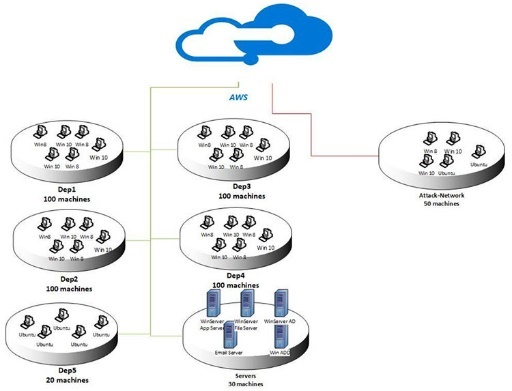
\includegraphics[width=0.75\linewidth]{fig/aws-ids2018.png}
	\caption{Mô hình mạng trong CSE-CIC-IDS2018}
	\label{fig:aws-ids2018}
\end{figure}

Các loại tấn công có trong dataset này bao gồm tấn công brute-force, tấn công heartbleed, Botnet, tấn công DoS, tấn công DDoS, tấn công Web, xâm nhập mạng từ bên trong.

Dataset được chia thành hai loại, thứ nhất là tập các tệp PCAP ghi nhận lưu lượng mạng và các mô tả về IP nguồn, IP đích và Protocol của các luồng tấn công và luồng hợp lệ, thứ hai là tập các tệp CSV được sinh ra từ phần mềm CICFlowMeter \cite{37-cicflowmeter} kèm với nhãn của các luồng đã được đánh dấu sẵn.

Do kích thước của các tệp PCAP rất lớn (lên tới hàng chục GB), nên trong khuôn khổ của khóa luận này, tôi sử dụng các tệp CSV đã được tạo sẵn với kích thước nhỏ hơn rất nhiều.

Dataset được chia ra thành từng ngày, mỗi ngày sẽ có một số loại tấn công được triển khai. Vì vậy, tôi chỉ chọn ra những ngày có tấn công DoS/DDoS được triển khai.

Danh sách các ngày được chọn trong bảng \ref{tab:day-choice-ids2018}.

\begin{table}[ht!]
\centering
	\begin{tabular}{|l|l|}
		\hline
		\multicolumn{1}{|c|}{\textbf{Ngày}} & \multicolumn{1}{c|}{\textbf{Mô tả}}                                                  \\ \hline
		Thurs-15-02-2018 & \begin{tabular}[c]{@{}l@{}}DoS-GoldenEye       \\    \\ DoS-Slowloris\end{tabular}   \\ \hline
		Fri-16-02-2018                      & \begin{tabular}[c]{@{}l@{}}DoS-SlowHTTPTest\\    \\ DoS-Hulk\end{tabular}   \\ \hline
		Tues-20-02-2018  & \begin{tabular}[c]{@{}l@{}}DDoS attacks-LOIC-HTTP\\    \\ DDoS-LOIC-UDP\end{tabular} \\ \hline
		Wed-21-02-2018                      & \begin{tabular}[c]{@{}l@{}}DDOS-LOIC-UDP    \\    \\ DDOS-HOIC\end{tabular} \\ \hline
	\end{tabular}
\caption{Danh sách các ngày được chọn trong dataset CICIDS2018}
\label{tab:day-choice-ids2018}
\end{table}

\subsection{Tiền xử lý và thống kê dữ liệu}
\label{preprocessing-data}

\subsubsection{Tiền xử lý}

Dữ liệu trong dataset không thật sự hoàn hảo, lý do đến từ phần CICFlowMeter vẫn còn một vài lỗi dẫn đến xuất hiện một số bản ghi trong dữ liệu chứa giá trị vô cực (Inf) hoặc không phải số (NaN). Vì vậy, bước cần thiết là loại bỏ các bản ghi lỗi này ra khỏi dataset.

Giải thuật tiền xử lý dữ liệu được mô tả trong lưu đồ \ref{fig:drop-line}.

\begin{figure}[ht!]
	\centering
	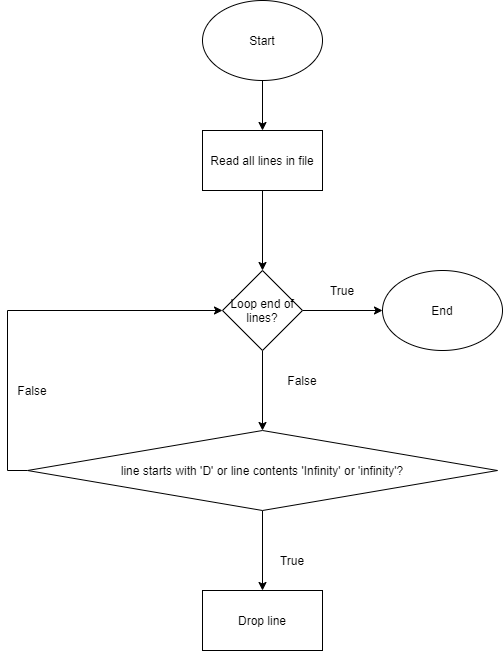
\includegraphics[width=0.75\linewidth]{fig/drop-line.png}
	\caption{Lưu đồ giải thuật tiền xử lý dataset}
	\label{fig:drop-line}
\end{figure}

\subsubsection{Thống kê}

Sau khi tiền xử lý dữa liệu, số lượng luồng hợp lệ và tấn công còn lại được ghi trong bảng \ref{tab:stat-ids2018}.

\begin{table}[ht!]
\centering
	\begin{tabular}{|l|l|l|}
		\hline
		\multicolumn{1}{|c|}{\textbf{Ngày}} & \multicolumn{1}{c|}{\textbf{Số luồng hợp lệ}} & \multicolumn{1}{c|}{\textbf{Số luồng tấn công}} \\ \hline
		Thurs-15-02-2018 & 987,980   & 52,498  \\ \hline
		Fri-16-02-2018   & 446,772   & 601,802 \\ \hline
		Tues-20-02-2018  & 7,313,104 & 576,191 \\ \hline
		Wed-21-02-2018   & 360,833   & 687,742 \\ \hline
	\end{tabular}
\caption{Bảng thống kê dữ liệu trong CICIDS2018}
\label{tab:stat-ids2018}
\end{table}

\subsection{Xử lý dữ liệu}

\subsubsection{Phân chia dữ liệu thành các tập con}

Vì mỗi một ngày chứa lưu lượng của một loại tấn công khác nhau, nên trước khi gộp dữ liệu các ngày lại với nhau, tôi tiến hành phân chia dữ liệu trên từng ngày thành 2 tập là tập huấn luyện và tập kiểm tra với tỷ lệ 8:2. Sau đó, tôi ghép các tập con này lại và thu được dataset đặt tên là \textbf{IDS-train} tương ứng với tập huấn luyện và \textbf{IDS-test} tương ứng với tập kiểm tra được thống kê trong bảng \ref{tab:sub-dataset}. Trước khi ghép các dữ liệu lại với nhau, tôi đã loại bỏ trường "Timestamp", vì trường này không quan trọng cho việc phân tích và huấn luyện.

\begin{table}[ht!]
\centering
	\begin{tabular}{|l|l|l|}
		\hline
		\multicolumn{1}{|c|}{\textbf{Tập}} & \multicolumn{1}{c|}{\textbf{Số luồng hợp lệ}} & \multicolumn{1}{c|}{\textbf{Số luồng tấn công}} \\ \hline
		IDS-train                          & 7,287,007                                     & 1,534,586                                       \\ \hline
		IDS-test                           & 1,821,682                                     & 383,647                                         \\ \hline
	\end{tabular}
\caption{Các tập dữ liệu con sau khi phân chia}
\label{tab:sub-dataset}
\end{table}

\subsubsection{Phân tích, tối ưu hóa dữ liệu}

Sau khi đã có dataset cuối cùng, tôi tiến hành phân tích và tối ưu dữ liệu để phục vụ cho việc huấn luyện.

\textit{Phân tích}

Tổng số đặc trưng mà CICFlowMeter trích xuất là 84, tuy nhiên khi tác giả công bố dataset đã bỏ đi một vài đặc trưng như Source IP, Source Port, Dest IP, vv, và thêm một đặc trưng được tôi loại bỏ là ''Timestamp'' nên tổng số đặc trưng còn lại là 78. Chi tiết các đặc trưng này trong bảng \ref{tab:feature-list}.

\begin{center}
	\centering
	\begin{longtable}{|l|l|l|}
		\hline
		\multicolumn{1}{|c|}{\textbf{STT}} & \multicolumn{1}{c|}{\textbf{Đặc trưng}} & \multicolumn{1}{c|}{\textbf{Mô tả}} \\ \hline
		1  & Dst Port          & Cổng   của địa chỉ IP đích trong gói tin IP        \\ \hline
		2  & Protocol          & Giao   thức mạng với 6 là TCP, 17 là UDP           \\ \hline
		3  & Flow Duration     & Tổng   thời gian của luồng                         \\ \hline
		4  & Tot Fwd Pkts      & Tổng   số gói tin trong luồng theo chiều tới (fwd) \\ \hline
		5  & Tot Bwd Pkts      & Tổng   số gói tin trong luồng theo chiều lui (bwd) \\ \hline
		6  & TotLen Fwd Pkts   & Tổng   độ dài của các gói tin fwd                  \\ \hline
		7  & TotLen Bwd Pkts   & Tổng   độ dài của các gói tin bwđ                  \\ \hline
		8  & Fwd Pkt Len Max   & Độ   dài max gói tin fwd                           \\ \hline
		9  & Fwd Pkt Len Min   & Độ   dài min gói tin fwd                           \\ \hline
		10 & Fwd Pkt Len Mean  & Mean   độ dài gói tin fwd                          \\ \hline
		11 & Fwd Pkt Len Std   & Độ   lệch chuẩn độ dài gói tin fwd                 \\ \hline
		12 & Bwd Pkt Len Max   & Độ   dài max gói tin bwd                           \\ \hline
		13 & Bwd Pkt Len Min   & Độ   dài min gói tin bwd                           \\ \hline
		14 & Bwd Pkt Len Mean  & Mean   độ dài gói tin bwd                          \\ \hline
		15 & Bwd Pkt Len Std   & Độ   lệch chuẩn độ dài gói tin bwd                 \\ \hline
		16 & Flow Byts/s       & Tổng   số bytes trong luồng / giây                 \\ \hline
		17 & Flow Pkts/s       & Tổng   số gói tinn trong luồng / giây              \\ \hline
		18 & Flow IAT Mean     & Mean   IAT luồng                                   \\ \hline
		19 & Flow IAT Std      & Độ   lệch chuẩn IAT luồng                          \\ \hline
		20 & Flow IAT Max      & Max   IAT luồng                                    \\ \hline
		21 & Flow IAT Min      & Min   IAT luồng                                    \\ \hline
		22 & Fwd IAT Tot       & Tổng   số IAT fwd                                  \\ \hline
		23 & Fwd IAT Mean      & Mean   IAT fwd                                     \\ \hline
		24 & Fwd IAT Std       & Độ   lệch chuẩn IAT fwd                            \\ \hline
		25 & Fwd IAT Max       & Max   IAT fwd                                      \\ \hline
		26 & Fwd IAT Min       & Min   IAT fwd                                      \\ \hline
		27 & Bwd IAT Tot       & Tổng   số IAT bwd                                  \\ \hline
		28 & Bwd IAT Mean      & Mean   IAT bwd                                     \\ \hline
		29 & Bwd IAT Std       & Độ   lệch chuẩn IAT bwd                            \\ \hline
		30 & Bwd IAT Max       & Max   IAT bwd                                      \\ \hline
		31 & Bwd IAT Min       & Min   IAT bwd                                      \\ \hline
		32 & Fwd PSH Flags     & Tổng   số cờ PSH fwd                               \\ \hline
		33 & Bwd PSH Flags     & Tổng   số cờ PSH bwd                               \\ \hline
		34 & Fwd URG Flags     & Tổng   số cờ URG fwd                               \\ \hline
		35 & Bwd URG Flags     & Tổng   số cờ URG bwd                               \\ \hline
		36 & Fwd Header Len    & Tổng   độ dài header các gói tin fwd               \\ \hline
		37 & Bwd Header Len    & Tổng   độ dài header các gói tin bwd               \\ \hline
		38 & Fwd Pkts/s        & Tổng   số gói tin fwd / giây                       \\ \hline
		39 & Bwd Pkts/s        & Tổng   số gói tin bwd / giây                       \\ \hline
		40 & Pkt Len Min       & Độ   dài min gói tin trong luồng                   \\ \hline
		41 & Pkt Len Max       & Độ   dài max gói tin trong luồng                   \\ \hline
		42 & Pkt Len Mean      & Độ   dài mean gói tin trong luồng                  \\ \hline
		43 & Pkt Len Std       & Độ   lệch chuẩn độ dài gói tin trong luồng         \\ \hline
		44 & Pkt Len Var       & Phương   sai độ dài gói tin trong luồng            \\ \hline
		45 & FIN Flag Cnt      & Tổng   số cờ FIN                                   \\ \hline
		46 & SYN Flag Cnt      & Tổng   số cờ SYN                                   \\ \hline
		47 & RST Flag Cnt      & Tổng   số cờ RST                                   \\ \hline
		48 & PSH Flag Cnt      & Tổng   số cờ PSH                                   \\ \hline
		49 & ACK Flag Cnt      & Tổng   số cờ ACK                                   \\ \hline
		50 & URG Flag Cnt      & Tổng   số cờ URG                                   \\ \hline
		51 & CWE Flag Count    & Tổng   số cờ CWE                                   \\ \hline
		52 & ECE Flag Cnt      & Tổng   số cờ ECE                                   \\ \hline
		53 & Down/Up Ratio     & Lưu   lượng fwd / lưu lượng bwd                    \\ \hline
		54 & Pkt Size Avg      & Kích   thước trung bình của gói tin                \\ \hline
		55 & Fwd Seg Size Avg  & Kích   thước trung bình gói tin fwd                \\ \hline
		56 & Bwd Seg Size Avg  & Kích   thước trung bình gói tin bwd                \\ \hline
		57 & Fwd Byts/b Avg    & Số   bytes/bulk trung bình fwd                     \\ \hline
		58 & Fwd Pkts/b Avg    & Số   gói tin/bulk trung bình fwd                   \\ \hline
		59 & Fwd Blk Rate Avg  & Tỷ   lệ bulk fwd trung bình                        \\ \hline
		60 & Bwd Byts/b Avg    & Số   bytes/bulk bwd                                \\ \hline
		61 & Bwd Pkts/b Avg    & Số   gói tin/bulk bwd                              \\ \hline
		62 & Bwd Blk Rate Avg  & Tỷ   lệ bulk bwd trung bình                        \\ \hline
		63 & Subflow Fwd Pkts  & Số   gói tin trong luồng con fwd                   \\ \hline
		64 & Subflow Fwd Byts  & Số   bytes trong luồng con fwd                     \\ \hline
		65 & Subflow Bwd Pkts  & Số   gói tin trong luồng con bwd                   \\ \hline
		66 & Subflow Bwd Byts  & Số   bytes trong luồng con  bwd                    \\ \hline
		67 & Init Fwd Win Byts & TCP   window size của gói tin đầu tiên fwd         \\ \hline
		68 & Init Bwd Win Byts & TCP   window size của gói tin đầu tin bwd          \\ \hline
		69 & Fwd Act Data Pkts & Số   gói tin thật sự có payload fwd                \\ \hline
		70 & Fwd Seg Size Min  & Kích   thước header nhỏ nhất fwd                   \\ \hline
		71 & Active Mean       & Mean   thời gian active                            \\ \hline
		72 & Active Std        & Độ   lệch chuẩn thời gian active                   \\ \hline
		73 & Active Max        & Max   thời gian active                             \\ \hline
		74 & Active Min        & Min   thời gian active                             \\ \hline
		75 & Idle Mean         & Mean   thời gian idle                              \\ \hline
		76 & Idle Std          & Độ   lệch chuẩn thời gian idle                     \\ \hline
		77 & Idle Max          & Max   thời gian idle                               \\ \hline
		78 & Idle Min          & Min   thời gian idle                               \\ \hline
	\caption{Danh sách các đặc trưng của luồng gói tin được rút trích}
	\label{tab:feature-list}
	\end{longtable}
\end{center}

\textit{Tối ưu hóa}

Tôi sử dụng phương pháp Feature Selection với hàm ChiSquare để chọn ra các đặc trưng thật sự cần thiết cho việc huấn luyện.
Tôi sử dụng thư viện scikit-learn để thực hiện. Giải thuật được mô tả trong sơ đồ hình \ref{fig:feature-selection}.

\begin{figure}[ht!]
	\centering
	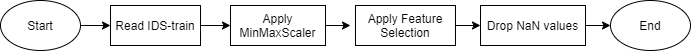
\includegraphics[width=\linewidth]{fig/feature-selection.png}
	\caption{Lưu đồ tối ưu hóa dataset}
	\label{fig:feature-selection}
\end{figure}

Từ đó tôi loại bỏ được 11 đặc trưng gồm Dst Port, Bwd PSH Flags, Fwd URG Flags, Bwd URG Flags, CWE Flag Count, Fwd Byts/b Avg, Fwd Pkts/b Avg, Fwd Blk Rate Avg, Bwd Byts/b Avg, Bwd Pkts/b Avg, Bwd Blk Rate Avg. Từ đó còn lại 67 đặc trưng cho việc huấn luyện.

\section{Các mô hình huấn luyện}

Trước khi áp dụng huấn luyện, tôi chuyển các giá trị âm trong dữ liệu thành 0, sau đó thực hiện normalize dữ liệu bằng hàm normalize trong thư viện Keras. Hàm này sử dụng L2 norm để normalize dữ liệu.

\subsection{Các chỉ số đánh giá mô hình}

Trong bài toán hiện tại tôi đang giải quyết là bài toán phân lớp nhị phân, vì vậy kết quả đầu ra là Positive (Attack) hay Negative (Benign).
Ma trận nhầm lẫn (Confusion matrix) của tôi sẽ có dạng như bảng \ref{tab:confusion_matrix_pattern}. Với TP, FP, TN, FN tương ứng với True Positive, False Positive, True Negative, False Negative.

\begin{table}[ht!]
\centering
	\begin{tabular}{|l|l|l|l|}
		\hline
		&                   & \textbf{Predicted} &                   \\ \hline
		&                   & \textit{Negative}  & \textit{Positive} \\ \hline
		\textbf{True} & \textit{Negative} & \# of TN           & \# of FP          \\ \hline
		& \textit{Positive} & \# of FN           & \# of TP          \\ \hline
	\end{tabular}
\caption{Mẫu ma trận nhầm lẫn}
\label{tab:confusion_matrix_pattern}
\end{table}

Khi đó, công thức của các chỉ số đánh giá như sau.

\textit{Accuracy}: 
\[ Acc = \frac{TP + TN}{Total} \]
\textit{Precision} (hay Positive predictive value):
\[ Pre = \frac{TP}{TP + FP} \]
\textit{Recall}:
\[ Rec = \frac{TP}{TP + FN} \]
\textit{F1-score}:
\[ F1 = 2 \frac{Pre \cdot Rec}{Pre + Rec} \]

\subsection{Mô hình học máy}

Trong phần này, tôi giới thiệu chi tiết các mô hình học máy gồm Support Vector Machine, Naïve Bayes, Decision Tree.

\subsubsection{Support Vector Machine}

Tham khảo từ nghiên cứu \cite{67-Patle} của A. Patle và cộng sự, SVM phân loại lớp bằng việc tạo ra một siêu phẳng (hyperplane) N chiều. SVM là một thực thể toán học, một giải thuật để tối đa hóa một hàm toán học cụ thể đối với một tập dữ liệu nhất định. SVM có 4 khái niệm cơ bản:

\begin{itemize} 
	\item[--] Siêu phẳng phân chia (Separating hyperplane)
	\item[--] Siêu phẳng biên cực đại (Maximum-margin hyperplane)
	\item[--] Biên mềm (Soft Margin)
	\item[--] Hàm cốt lõi (Kernel function)  
\end{itemize}
 
 \textit{Biên}
 
 Biên là khoảng cách giữa siêu phẳng đến hai điểm dữ liệu gần nhất tương ứng với các phân lớp.
 
 \textit{Siêu phẳng phân chia}
 
 Đường thẳng chia không gian thành 2 phần, và ở không gian ba chiều chúng ta cần mặt phẳng để phân chia không gian. Định nghĩa chung cho ranh giới phân chia trong không gian N chiều là siêu phẳng. Vì vậy, siêu phẳng phân chia là ranh giới về cơ bản phân chia các mẫu khác nhau trong tập dữ liệu. Hình \ref{fig:separating-hyperplane} ví dụ một siêu phẳng phân chia.
 
 \begin{figure}[ht!]
 	\centering
 	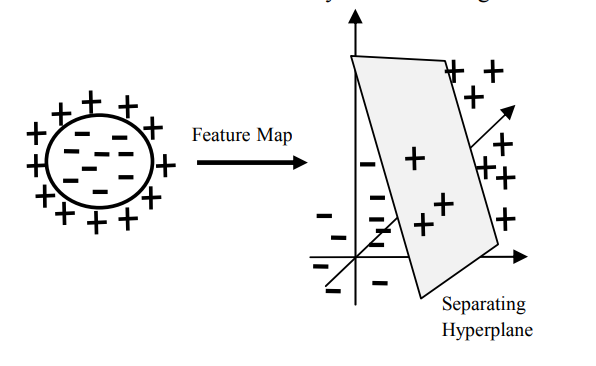
\includegraphics[width=0.5\linewidth]{fig/separating-hyperplane.png}
 	\caption{Ví dụ siêu phẳng phân chia}
 	\label{fig:separating-hyperplane}
 \end{figure}

\textit{Siêu phẳng biên cực đại (siêu phẳng tối ưu)}

Siêu phẳng biên cực đại nghĩa là lựa chọn ranh giới ở chính giữa. Nói cách khác, ranh giới được chọn để phân chia hai lớp phải đáp ứng được biên là lớn nhất.

Theo \cite{68-Vapnik}, cách giải thích của Vapnik và cộng sự trình bày về khái niệm này như sau. Ta có một tập huấn luyện được gán nhãn

\begin{gather}
	\label{svm:1}
	(y_1, x_1), ... , (y_l, x_l), y_i \in {-1, 1}
\end{gather}

được xem là có thể phân chia tuyến tính nếu tồn tại một vec-tơ \( \textbf{w} \) một đại lượng vô hướng \( \textit{b}\) sao cho các bất bất đẳng thức

\begin{equation}
	\begin{gathered}
	\label{svm:2}
		w \cdot x_i + \textit{b} \geq 1 \quad \quad \quad \quad if \quad \quad y_i = 1, \\
		w \cdot x_i + \textit{b} \leq 1 \quad \quad \quad \quad if \quad \quad y_i = -1
	\end{gathered}
\end{equation}

đều thỏa tất cả phần tử trong tập huấn luyện (\ref{svm:1}). Viết lại bất đẳng thức (\ref{svm:2})

\begin{gather}
	\label{svm:3}
	y_i (w \cdot x_i + \textit{b}) \geq 1, \quad \quad \quad i = 1, ..., l
\end{gather}

Siêu phẳng tối ưu

\begin{gather}
	\label{svm:4}
	w_0 \cdot x + \textit{b}_0 = 0
\end{gather}

là siêu phẳng duy nhất chia dữ liệu huấn luyện với biên lớn nhất: nó xác định hướng của \textbf{w}/|\textbf{w}| sao cho khoảng cách khoảng cách hình chiếu của vec-tơ huấn luyện của hai lớp khác nhau là tối đa.

\textit{Biên mềm}

SVM có thể chịu được lỗi trong dữ liệu bằng cách cho phép một vài dữ liệu bị phân lớp sai. Để làm được vậy, giải thuật SVM chỉnh sửa và thêm vào “biên mềm” (Hình \ref{fig:svm-soft-margin}). Cơ bản, điều này cho phép một số điểm dữ liệu di chuyển qua rìa của siêu phẳng phân chia mà không ảnh hưởng đến kết quả cuối cùng. Trong hình \ref{fig:svm-soft-margin}, siêu phẳng là B1 và B2. B1 tốt hơn B2 vì nó tối đa hóa biên. 

\begin{figure}[ht!]
	\centering
	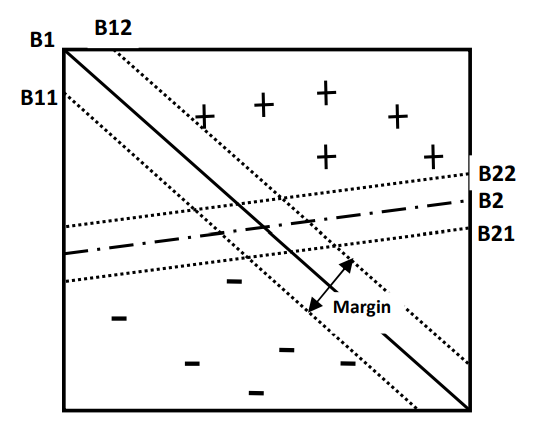
\includegraphics[width=0.5\linewidth]{fig/svm-soft-margin.png}
	\caption{Ví dụ biên mềm}
	\label{fig:svm-soft-margin}
\end{figure}

\textit{Hàm cốt lõi}

Hàm cốt lõi là thủ thuật toán học cho phép SVM phân lớp trong không gian hai chiều của một tập dữ liệu ở không gian một chiều. Nói chung, một hàm cốt lõi ánh xạ dữ liệu từ một không gian chiều thấp đến một không gian có chiều cao hơn. Công thức bên dưới và hình \ref{fig:svm-kernel} thể hiện cách hàm cốt lõi ánh xạ dữ liệu.

\[ \langle x_1 \cdot x_2 \rangle \leftarrow K(x_1,x_2) = \langle \Phi(x_1) \cdot \Phi(x_2) \rangle \]

 \begin{figure}[ht!]
 	\centering
	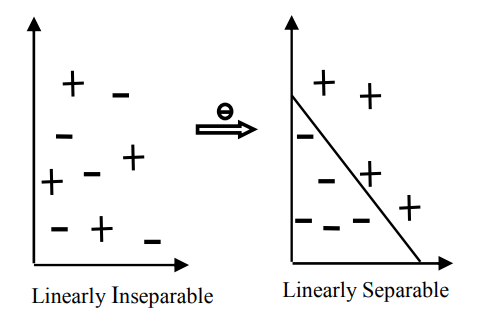
\includegraphics[width=0.5\linewidth]{fig/svm-kernel.png}
	\caption{Cách hàm cốt lõi ánh xạ dữ liệu}
	\label{fig:svm-kernel}
\end{figure}

\textit{Hàm cốt lõi tuyến tính (Linear Kernel Function)}

Hàm cốt lõi tuyến tính được biểu diễn như sau: \( K(x, x_j) = x \cdot x^T\)

\subsubsection{Naïve Bayes}

Theo nghiên cứu của Rish và các cộng sự \cite{71-Rish}, giải thuật phân lớp Naïve được diễn giải như sau.

Cho \( X = X_1, ..., X_n\) là một vec-tơ những biến ngẫn nhiên, được gọi là đặc trưng, với mỗi đặc tính lấy giá trị tiền miền $D_i$ của nó. Tập tất cả các vec-tơ đặc trưng được ký hiệu  \(\Omega = D_1 \times ... \times D_n\). Cho $C$ là một biến ngẫu nhiên không quan sát ký hiệu cho phân lớp của mẫu, $C$ có thể giữa một giá trị trong $m$ giá trị $c \in {0,...,m-1}$.

Một hàm \(g: \Omega \rightarrow {0,...,m-1}\), với $g(x) = C$ ký hiệu một \textit{khái niệm} được học. 

Một  máy phân lớp được định nghĩa bởi một hàm $h: \Omega \rightarrow {0,...,m-1}$ (một hypothesis) gán một lớp cho bất cứ mẫu được cho nào. Một hướng tiếp cận thông dụng là liên kết mỗi lớp $i$ với một hàm phân biệt \( f_i(X), i={0,...,m-1}\), và để cho máy phân lớp chọn phân lớp với hàm phân biệt lớn nhất trên một mẫu được cho: \(h(x)  = argmax_{i \in {0,...,m-1}f_i(x)}\).

Máy phân lớp Bayes $h*(x)$ được sử dụng như những hàm phân biệt xác xuất có điều kiện của các vec-tơ đặc trưng được cho. Áp dụng luật Bayes, hàm phân biệt: 

\[ f^{*}_i(x) = P(X=x|C=i)P(C=i)\] 

với $P(X=x|C=i)$ được gọi là \textit{phân phối xác xuất có điều kiện}. Vì vậy máy phân lớp Bayes:

\[ h^{*}(x)  = argmax_i P(X=x|C=i)P(C=i)\]

Tuy nhiên, trực tiếp ước lượng P(X=x|C=i) thường  khó trong các tập đặc trưng có không gian bậc cao. Vì vậy để đơn giản, ta sử dụng \textit{native Bayes} (NB(x)) với hàm phân biệt được định  nghĩa như sau:

\[ f^{NB}_i = \Pi^n_{j=1}P(X_j=x_j|C=i)P(C=i)\]

\subsubsection{Decision Tree}

Theo nghiên cứu của Somvanshi và các cộng sự \cite{72-Somvanshi}, Decision Tree (DT) được diễn giải như sau.

Để tạo ra các nút, DT sử dụng phương pháp tăng thông  tin để xác định thuộc tính phù hợp trong cây. Từ mức thông tin cao nhất  chúng ta có thể chọn ra thuộc tính.  Có những giải thuật  DT khác nhau  mà trong đó ID3 (được giới thiệu bởi QUINLAN vào năm 1986) là giải thuật quan trọng dựa trên entropy thông tin để tạo ra giải thuật học có giám sát.

ID3 sử dụng thông tin tăng cường để quyết định phân chia thuộc tính. Đưa ra một tập hợp các kết quả, dữ liệu không chắc chắn biểu diễn trong tập dữ liệu được đo bởi công thức 

\[Entropy(S) = -\sum p(x)log2p(x\]

Với S là tập dữ liệu cho mỗi entropy được tính toán, X là tập hợp của các lớp trong tập dữ liệu, P(x) là xác suất của số phần tử trong lớp X đến số phần tử trong tập S. Khi I(S) = 0 thì tập dữ liệu được phân lớp hoàn hảo.

\subsubsection{Huấn luyện mô hình trên tập IDS-train}

Để đơn giản trong việc triển khai huấn luyện, tôi sử dụng thư viện Scikit-learn.

Với giải thuật SVM tôi huấn luyện với hàm cốt lõi tuyến tính (LSVM) với hàm LinearSVC. Bên cạnh đó tôi sử dụng hàm GaussianNB cho giải thuật Naïve Bayes (NB), hàm DecisionTreeClassifier cho giải thuật  Decision Tree (DT) và hàm RandomForestClassifier cho giải thuật Random Forest (RF).

\subsubsection{Kiểm thử mô hình trên tập IDS-test}

Kiểm thử  các mô hình đã huấn luyện ở trên, tôi thu được kết quả được thể hiện trong bảng \ref{tab:machine-learning-models-result}. Dựa vào kết quả trong bảng này, tôi nhận thấy giải thuật Decision Tree cho kết quả các chỉ số cao hơn hẳn các giải thuật còn lại, cho thấy tính hiệu quả của cách tiếp cận đơn giản mà giải thuật này áp dụng.

\begin{table}[ht!]
	\centering
	\begin{tabular}{|l|l|l|l|l|}
		\hline
		\multicolumn{1}{|c|}{\textbf{Mô hình}} &
		\multicolumn{1}{c|}{\textbf{Accuracy (\%)}} &
		\multicolumn{1}{c|}{\textbf{Precision (\%)}} &
		\multicolumn{1}{c|}{\textbf{Recall (\%)}} &
		\multicolumn{1}{c|}{\textbf{F1-score (\%)}} \\ \hline
		LSVM    & 95.67 & 88.05 & 86.91 & 87.48 \\ \hline
		NB      & 67.69 & 34.92 & 99.31 & 51.67 \\ \hline
		DT      & \textbf{99.97} & \textbf{99.91} & \textbf{99.94} & \textbf{99.92} \\ \hline
		RF      & 99.83 & 99.11 & 99.94 & 99.52 \\ \hline
	\end{tabular}
	\caption{Kết quả huấn luyện các mô hình học máy trên tập IDS-Test}
	\label{tab:machine-learning-models-result}
\end{table}

\subsection{Mô hình học sâu}

Ở các nghiên cứu \cite{27-Corin}, \cite{28-Yuan} với việc áp dụng các mô hình CNN và RNN mang lại kết quả tốt. Tuy nhiên, các nghiên cứu đó sắp xếp và xử lý dữ liệu theo thời gian (time series), từ đó việc xử dụng mạng nơ-ron tích chập rất hiệu quả trong việc rút trích đặc trưng. Trong khi đó, trong khóa luận này, đặc trưng của luồng dữ liệu đã được tôi xử lý như trình bày trong mục \ref{preprocessing-data}, vì vậy, tôi sẽ áp dụng mô hình DNN như trong nghiên cứu \cite{61-Basnet} để huấn luyện, và dùng mô hình này đại diện cho tiếp cận học sâu mà tôi muốn hướng tới.

Trước hết, tôi sẽ trình bày về các mô hình được đề xuất trong nghiên cứu \cite{27-Corin} và \cite{28-Yuan}.

\subsubsection{Chi tiết mô hình DeepDefense và LUCID}

\textit{Mô hình DeepDefense}\cite{28-Yuan}

Trong nghiên cứu này, tác giả sử dụng nhiều mô hình RNN khác nhau để đánh giá về độ chính xác trên hai dataset lớn (Data15) và dataset nhỏ (Data14) được thu thập từ dataset ISCX 2012 \cite{35-Shiravi}. Các mô hình gồm LSTM, GRU, CNNLSTM (kết hợp CNN để rút trích đặt trưng trước khi đến lớp LSTM), và 3LSTM. Các mô hình này đều cho kết quả state-of-the-art trên dataset mà tác giả huấn luyện, mà ở đó, mô hình 3LSTM có kiến trúc phức tạp nhất cho kết quả với độ chính xác cao nhất trên dataset lớn (98.41\%), trong khi mô hình GRU đơn giản hơn đạt được độ chính xác cao nhất trong dataset nhỏ (98.342\%). Kiến trúc các mô hình này được miêu tả như bảng trong hình \ref{fig:deep-defense-architecture}.

 \begin{figure}[ht!]
	\centering
	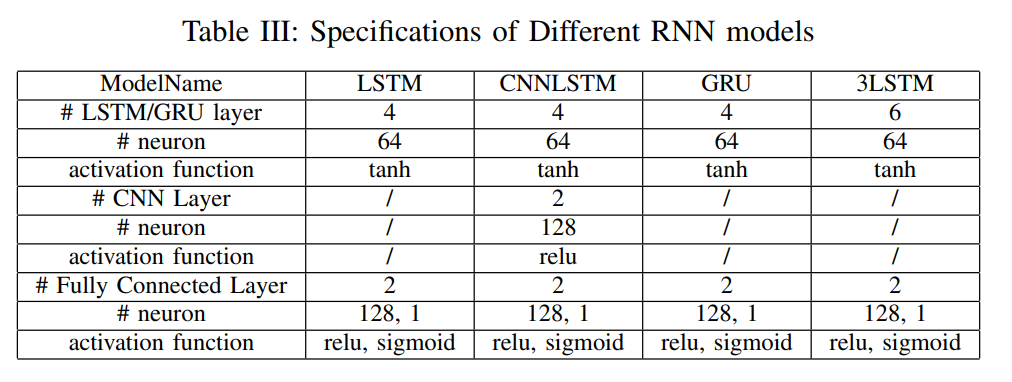
\includegraphics[width=\linewidth]{fig/deep-defense-architecture.png}
	\caption{Kiến trúc các mô hình của DeepDefense \cite{28-Yuan}}
	\label{fig:deep-defense-architecture}
\end{figure}

\textit{Mô hình LUCID}\cite{27-Corin}

Trong nghiên cứu này, tác giả tận dụng sự đơn giản mà hiệu quả của lớp Conv1D và Max  Pooling trong mạng CNN. Để xây dựng dataset, tác giả rút trích 11 đặc trưng của các gói tin và sắp xếp theo trình tự thời gian (time-series) với số lượng n cố định. Với các siêu tham số n (số lượng packet tối đa của 1 mẫu), t (thời gian quan sát tối đa 1 mẫu), k (số kernel của Conv1D), h (số filter của Conv1D), m (kích thước của Max Pooling), tác giả có thể tùy chỉnh các thông số này sao cho thu được mô hình có độ chính xác cao nhất. Cuối cùng với bộ siêu tham số n = 100, t = 100, k = 64, h = 3, m = 98, tác giả thu được độ chính xác mô hình trên dataset ISCX 2012 \cite{35-Shiravi} là 98.88\%. So với mô hình DeepDefense ở trên, mô hình LUCID có độ chính xác cao hơn và  đơn giản hơn nhiều lần. Kiến trúc của mô hình LUCID được thể hiện trong hình \ref{fig:lucid-model}.

\begin{figure}[ht!]
	\centering
	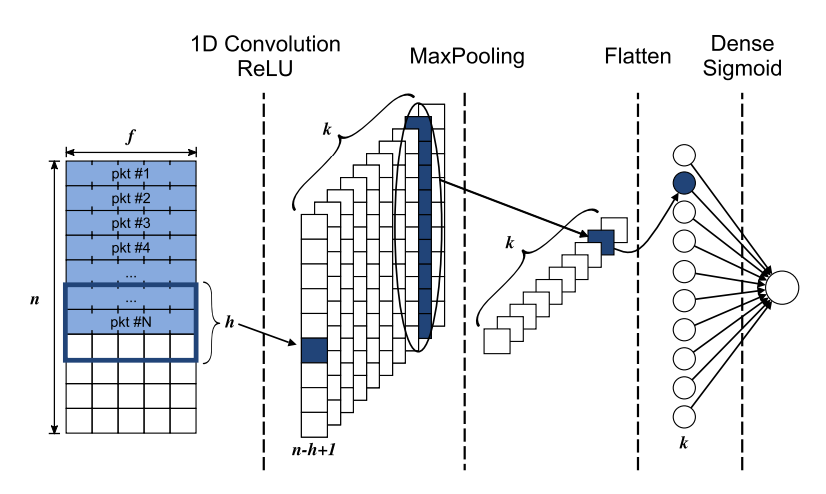
\includegraphics[width=0.6\linewidth]{fig/lucid-model.png}
	\caption{Kiến trúc mô hình của LUCID \cite{27-Corin}}
	\label{fig:lucid-model}
\end{figure}

\subsubsection{Chi tiết mô hình DNN}

Dựa theo nghiên cứu của Ram B. Basnet và các cộng sự \cite{61-Basnet}, mô hình tôi áp dụng được thể hiện trong hình \ref{fig:dnn-model}.

 \begin{figure}[ht!]
 	\centering
	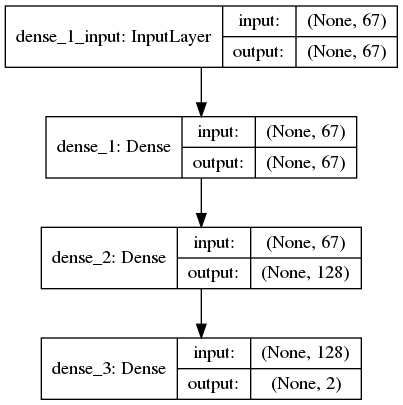
\includegraphics[width=0.5\linewidth]{fig/dnn-model.png}
	\caption{Mô hình học sâu DNN}
	\label{fig:dnn-model}
\end{figure}

Trong đó,

\begin{itemize}
	\item[--] Lớp Input: đầu vào có dạng (67,1) tương ứng với dạng của một bản ghi trong dataset có 67 đặc trưng của một luồng gói tin.
	\item[--] Lớp Dense\_1: lớp này có 67 đơn vị giúp rút trích đặc tính của từng đặc trưng trong dữ liệu. Hàm kích hoạt được dùng là ReLU.
	\item[--] Lớp Dense\_2: lớp này có 128 đơn vị. Hàm kích hoạt được dùng là ReLU.
	\item[--] Lớp Fully conntected (dense 3): lớp này có 2 đơn vị để để phân lớp Benign hay Attack. Hàm kích hoạt được dùng là Softmax.
\end{itemize}

\subsubsection{Huấn luyện mô hình DNN trên tập IDS-train}

Để huấn luyện mô hình, tôi sử dụng hàm tối ưu là Adam \cite{60-Kingma}, hàm mất mát là CategoricalCrossEntropy.

Trước khi huấn luyện, tôi tách tập \textit{IDS-train} thành hai phần là phần huấn luyện và phần xác thực với tỷ lệ 8:2. Sau khi huấn luyện với 10 epoch, tôi thu được kết quả với độ chính xác là 99.59\% trên tập xác thực.

Biểu đồ trong hình \ref{fig:dnn-train-acc} thể hiện độ chính xác và biểu đồ trong hình \ref{fig:dnn-train-loss} thể hiện sự mất mát trong quá trình huấn luyện.

\begin{figure}[!htb]
	\begin{minipage}{0.48\textwidth}
		\centering
		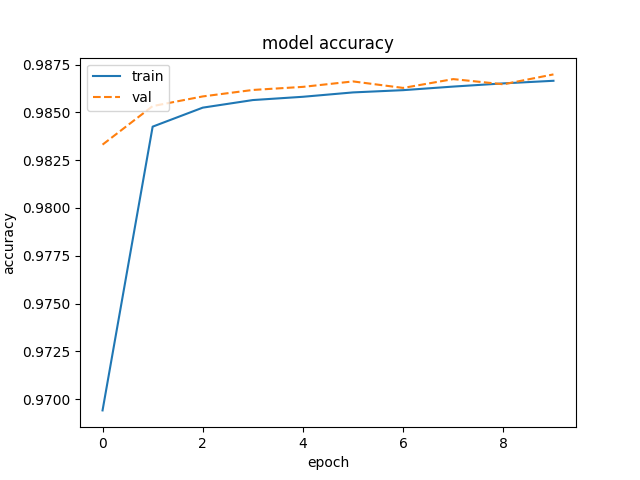
\includegraphics[width=\linewidth]{fig/dnn-train-acc.png}
		\caption{Độ chính xác mô hình DNN trong quá trình huấn luyện}
		\label{fig:dnn-train-acc}
	\end{minipage}\hfill
	\begin{minipage}{0.48\textwidth}
		\centering
		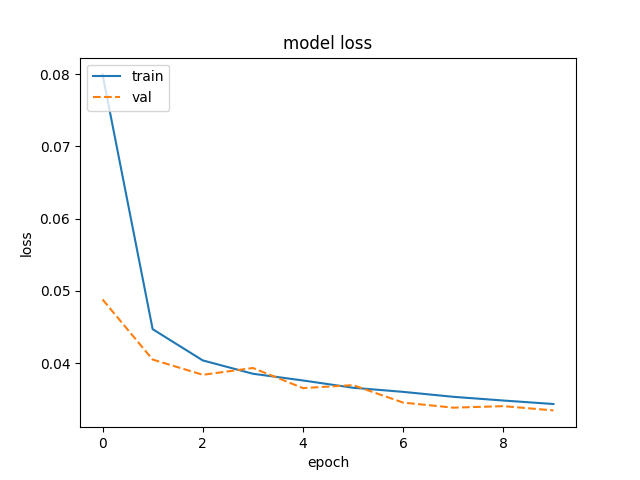
\includegraphics[width=\linewidth]{fig/dnn-train-loss.png}
		\caption{Độ mất mát mô hình DNN trong quá trình huấn luyện}
		\label{fig:dnn-train-loss}
	\end{minipage}
\end{figure}

\subsubsection{Kiểm thử mô hình DNN trên tập IDS-test}

Kiểm thử mô hình đã huấn luyện ở trên, tôi thu được kết quả đạt độ chính xác 99.22\%. Bảng \ref{tab:dnn-confusion-matrix} biểu thị ma trận nhầm lẫn.

\begin{table}[ht!]
	\centering
	\begin{tabular}{|l|l|l|l|}
		\hline
		&                   & \textbf{Predicted} &                   \\ \hline
		&                   & \textit{Negative}  & \textit{Positive} \\ \hline
		\textbf{True} & \textit{Negative} & 1,813,764          & 7,988             \\ \hline
		& \textit{Positive} & 9,291              & 374,356           \\ \hline
	\end{tabular}
\caption{Ma trận nhầm lẫn mô hình DNN trên tập IDS-Test}
\label{tab:dnn-confusion-matrix}
\end{table}

Từ ma trận nhầm lẫn, tôi có được các chỉ số đánh giá mô hình của mình trong bảng \ref{tab:dnn-result}.

\begin{table}[ht!]
	\centering
	\begin{tabular}{|l|l|l|l|l|}
		\hline
		\multicolumn{1}{|c|}{\textbf{Mô hình}} &
		\multicolumn{1}{c|}{\textbf{Accuracy (\%)}} &
		\multicolumn{1}{c|}{\textbf{Precision (\%)}} &
		\multicolumn{1}{c|}{\textbf{Recall (\%)}} &
		\multicolumn{1}{c|}{\textbf{F1-score (\%)}} \\ \hline
		DNN &
		99.22 &
		97.91 &
		97.58 &
		97.74 \\ \hline
	\end{tabular}
\caption{Kết quả mô hình DNN trên tập IDS-test}
\label{tab:dnn-result}
\end{table}

\subsubsection{So sánh kết quả mô hình DNN với DeepDefense và LUCID}

Vì các mô hình DeepDefense \cite{28-Yuan} và LUCID \cite{27-Corin} chưa được tôi cài đặt và kiểm thử trên một tập dữ liệu, vì vậy tôi sẽ so sánh kết quả của mô hình DNN của tôi với các kết quả được công bố trong các nghiên cứu trên. Kết quả so sánh được biểu thị trong bảng \ref{tab:dnn-comparision}.

\begin{table}[ht!]
	\begin{tabular}{|l|l|l|l|l|}
		\hline
		\multicolumn{1}{|c|}{\textbf{Mô hình}} &
		\multicolumn{1}{c|}{\textbf{Accuracy (\%)}} &
		\multicolumn{1}{c|}{\textbf{Precision (\%)}} &
		\multicolumn{1}{c|}{\textbf{Recall (\%)}} &
		\multicolumn{1}{c|}{\textbf{F1-score (\%)}} \\ \hline
		DNN         & \textbf{99.22} & 97.91          & 97.58          & 97.74          \\ \hline
		LUCID       & 98.88 & \textbf{98.27} & \textbf{99.52} & \textbf{98.89} \\ \hline
		DeepDefense & 98.41          & 98.34          & 98.48          & 98.41          \\ \hline
	\end{tabular}
\caption{So sánh kết quả của mô hình DNN với DeepDefense và LUCID}
\label{tab:dnn-comparision}
\end{table}

Từ số liệu trong bảng \ref{tab:dnn-comparision}, tôi nhận thấy, kết quả của các mô hình trên các tập kiểm thử của chính họ đều đạt được kết quả tốt và đạt được state-of-the-art.

\subsection{So sánh đánh giá các mô hình trên tập IDS-test}
\label{compare-multi-models}

Trong phần này, tôi sẽ so sánh các chỉ số đánh giá và thời gian thực thi giữa các mô hình học máy với mô hình học sâu DNN.

\subsubsection{So sánh đánh giá độ chính xác}

\begin{table}[ht!]
	\centering
	\begin{tabular}{|l|l|}
		\hline
		\multicolumn{1}{|c|}{\textbf{Mô hình}} & \multicolumn{1}{c|}{\textbf{Accuracy (\%)}} \\ \hline
		DT   & \textbf{99.97} \\ \hline
		RF   & \textbf{99.83} \\ \hline
		DNN  & 99.22          \\ \hline
		LSVM & 95.67          \\ \hline
		NB   & 67.69          \\ \hline
	\end{tabular}
\caption{So sánh độ chính xác của các mô hình trên tập IDS-Test}
\label{tab:compare}
\end{table}

 \begin{figure}[ht!]
 	\centering
	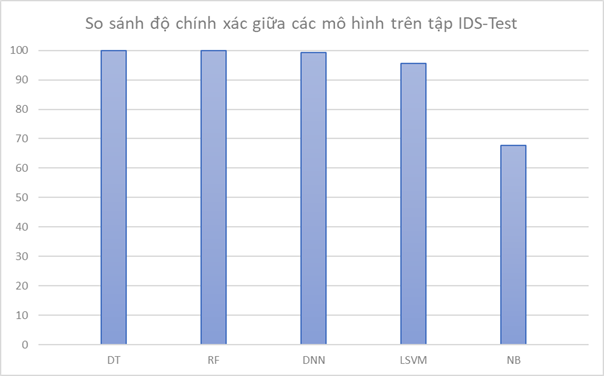
\includegraphics[width=\linewidth]{fig/compare-acc.png}
	\caption{So sánh độ chính xác các mô hình trên tập IDS-test}
	\label{fig:compare-acc}
\end{figure}

Từ bảng \ref{tab:compare} và biểu đồ hình \ref{fig:compare-acc}, có thể thấy, hai mô hình học máy có tiếp cận đơn giản là Decision Tree và Random Forest có độ chính xác cao hơn mô hình DNN. Điều này cho thấy sự đơn giản mà hiệu quả của các mô hình học máy trong việc nhận diện tấn công DoS/DDoS so với mô hình học sâu DNN có kiến trúc phức tạp và đòi hỏi nhiều tài nguyên tính toán hơn.

\subsubsection{So sánh và đánh giá thời gian thực thi}

Trong phần này tôi sẽ đánh giá thời gian thực thi giữa hai mô hình Decision Tree và DNN. Để đánh giá và so sánh thời gian thực thi của hai mô hình, tôi sử dụng phần cứng với CPU Intel Core I7-8700 và bộ nhớ RAM 32GB. Tổng số mẫu trong IDS-Test là 2,205,399 mẫu. Kết quả được biểu thị trong bảng \ref{tab:compare-runtime}.

\begin{table}[ht!]
	\centering
	\begin{tabular}{|l|l|l|}
		\hline
		\multicolumn{1}{|c|}{\textbf{Mô hình}} &
		\multicolumn{1}{c|}{\textbf{\begin{tabular}[c]{@{}c@{}}Thời gian \\ thực thi (giây)\end{tabular}}} &
		\multicolumn{1}{c|}{\textbf{\begin{tabular}[c]{@{}c@{}}Thời gian thực thi\\ trung bình 1 mẫu (giây)\end{tabular}}} \\ \hline
		DT &
		\textbf{0.4} &
		\textbf{$2 \cdot 10^{-7}$} \\ \hline
		DNN &
		8.5 &
		$4 \cdot 10^{-6}$  \\ \hline
	\end{tabular}
\caption{So sánh thời gian thực thi giữa DT và DNN}
\label{tab:compare-runtime}
\end{table}

Từ kết quả trong bảng \ref{tab:compare-runtime}, tôi nhận thấy thời gian thực thi mô hình Decision Tree nhanh hơn đáng kể so với mô hình DNN (gấp 22 lần). Từ đó cho thấy, Decision Tree không những vượt trội hơn DNN về độ chính xác mà còn vượt trội hơn cả về thời gian thực thi.

\section{Phát triển phần mềm phát hiện tấn công DoS/DDoS – IDS-DDoS}

Sau khi huấn luyên các mô hình học máy và học sâu, tôi tiến hành viết phần mềm phát hiện tấn công mạng trong thời gian thực.

\subsection{Kiến trúc của phần mềm}

Ý tưởng của phần mềm là sẽ lắng nghe các gói tin trên một giao diện mạng, khi phát hiện một luồng tấn công, thông báo sẽ được gửi lên một máy chủ thông qua unix socket. Lưu đồ của phần mềm được thể hiện trong hình \ref{fig:ids-software}.

\begin{figure}[ht!]
	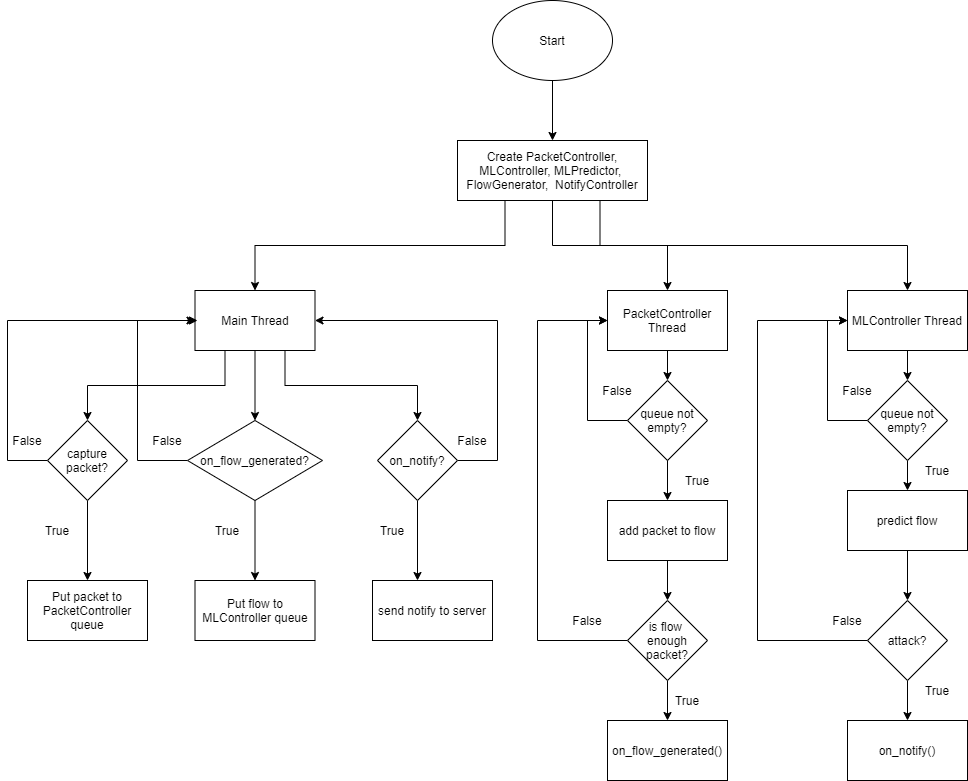
\includegraphics[width=\linewidth]{fig/ids-software.png}
	\caption{Lưu đồ phần mềm IDS-DDoS}
	\label{fig:ids-software}
\end{figure}

Phần mềm được thiết kế chạy đa tiểu trình (multi-thread). Trong đó có 3 tiểu trình là MainThread, PacketControllerThread và MLControllerThread.

\textit{MainThread}

Trong tiểu trình này, các gói tin sẽ được thu thập trên một giao diện mạng (một card mạng), cứ mỗi lần bắt được một gói tin, tiểu trình này sẽ đẩy thông tin gói tin đó vào trong hàng đợi (queue) của PacketControllerThread để chở xử lý tạo ra các luồng gói tin (flow). Bên cạnh đó, tiểu trình này có hai hàm callback là \textbf{on\_flow\_generated} và \textbf{on\_notify}. Mỗi khi PacketControllerThread tạo ra 1 flow mới, nó sẽ gọi hàm \textbf{on\_flow\_generated} để thông báo, khi nhận được thông báo MainThread sẽ đẩy flow này vào trong queue của MLControllerThread để chờ xử lý. Mỗi khi MLControllerThread xử lý xong, nó sẽ gọi hàm \textbf{on\_notify} để thông báo cho MainThread. Hàm \textbf{on\_notify} ở MainThread có chức năng là sẽ đẩy thông điệp đến một socket server thông qua unix socket.

\textit{PacketControllerThread}

Tiểu trình này sẽ có một vòng lặp vô tận kiểm tra xem queue có phần tử không, nếu có nó sẽ tiến hành lấy gói tin trong queue ra, biến đổi thành đối tượng lớp BasicPacketInfo, đối tượng này sẽ được xử lý trong lớp FlowGenerator. FlowGenerator sẽ liên tục đẩy các BasicPacketInfo vào đối tượng lớp BasicFlow cho đến khi nhận được gói tin kết thúc hoặc timeout. Cuối cùng nó sẽ đẩy đối tượng lớp BasicFlow vào hàm \textbf{on\_flow\_generated}.

\textit{MLControllerThread}

Tương tự PacketControllerThread, tiểu trình này cũng có một vòng lặp để kiểm tra queue, nếu có phần tử (flow) nó sẽ tiến hành phân loại flow này, nếu là flow độc hại (tấn công DoS/DDoS) nó sẽ gọi hàm \textbf{on\_notify}.

\subsection{Rút trích các đặc trưng}

Để rút trích đặc trưng của một luồng gói tin, tôi sử dụng 3 lớp là BasicPacketInfo, BasicFlow và FlowGenerator được mô tả như bên dưới. Toàn bộ giải thuật của các lớp này được tôi tham khảo mã nguồn phần mềm CICFlowMeter \cite{37-cicflowmeter}. Lý do là vì dataset mà tôi sử dụng để huấn luyện được tạo ra từ phần mềm này.

\textit{Lớp BasicPacketInfo}

Gói tin mạng có rất nhiều thành phần, vì vậy cần phải phân tích và lấy ra các thông tin thiết yếu. Các thông tin này sẽ được đưa vào lớp BasicPacketInfo. Các thông tin đó gồm: địa chỉ IP nguồn, địa chỉ IP đích, cổng nguồn, cổng đích, giao thức, timestamp, số lượng bytes trong payload, các flag FIN, PSH, URG, ECE, SYN, ACK, CWR, RST, TCP window, số byte trong header.

\textit{Lớp BasicFlow}

Từ thông tin của các BasicPacketInfo, lớp này sẽ tính toán các đặc trưng. Các đặc trưng này được liệt kê trong bảng \ref{tab:feature-list}. Các đặc trưng chủ yếu là các con số thống kê max, min, trung bình, độ lệch chuẩn và phương sai.

\textit{Lớp FlowGenerator}

Lưu đồ của lớp này được thể hiện trong hình \ref{fig:flow-gen}.

\begin{figure}[ht!]
	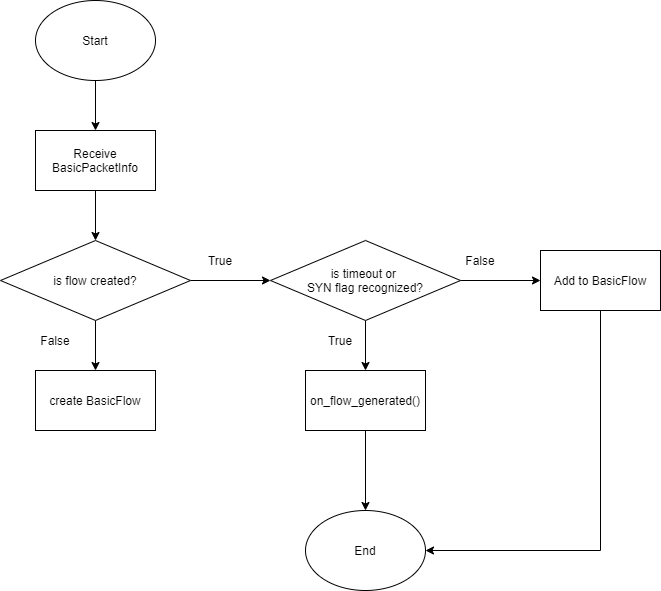
\includegraphics[width=\linewidth]{fig/flow-gen.png}
	\caption{Lưu đồ lớp FlowGenerator}
	\label{fig:flow-gen}
\end{figure}

\subsection{Sử dụng phần mềm}

Phần mềm có giao diện console. Để chạy được cần cung cấp các thông tin gồm giao diện mạng, đường dẫn đến unixsocket server, tên mô hình học máy/học sâu, các đường dẫn đến tệp lưu trữ mô hình.

python3 ids-ddos.py <network interface> <unixsocket path> <model name> <model path>

Ví dụ, lắng nghe trên eth0 và gửi qua socket /tmp/ids-ddos.

DT: \textit{python3 ids-ddos.py eth0 /tmp/ids-ddos svm ./model/dt\_model.pkl}

DNN: \textit{python3 ids-ddos.py eth0 /tmp/ids-ddos svm ./model/dnn-model.json,./model/dnn-weights.hdf5}

\section{Xây dựng SDN controller bằng RYU}
\label{traffic-monitor}

SDN controller của tôi được thiết kế để làm các nhiệm vụ:

\begin{itemize}
	\item[--] Là một switch controller cho các host trong mạng SDN.
	\item[--] Là một traffic monitor các gói tin đi và đến trong mạng, tín hiệu và dữ liệu này được gửi từ Open vSwitch.
	\item[--] Là một unixsocket server nhận tín hiệu từ phần mềm IDS-DDoS.
\end{itemize}

Lưu đồ trong hình \ref{fig:sdn-controller} thể hiện giải thuật của SDN controller, tuy nhiên tôi không thể hiện phần switch controller, vì đây là phần đơn giản được sao chép từ ví dụ của nhà phát triển.

\begin{figure}[ht!]
	\centering
	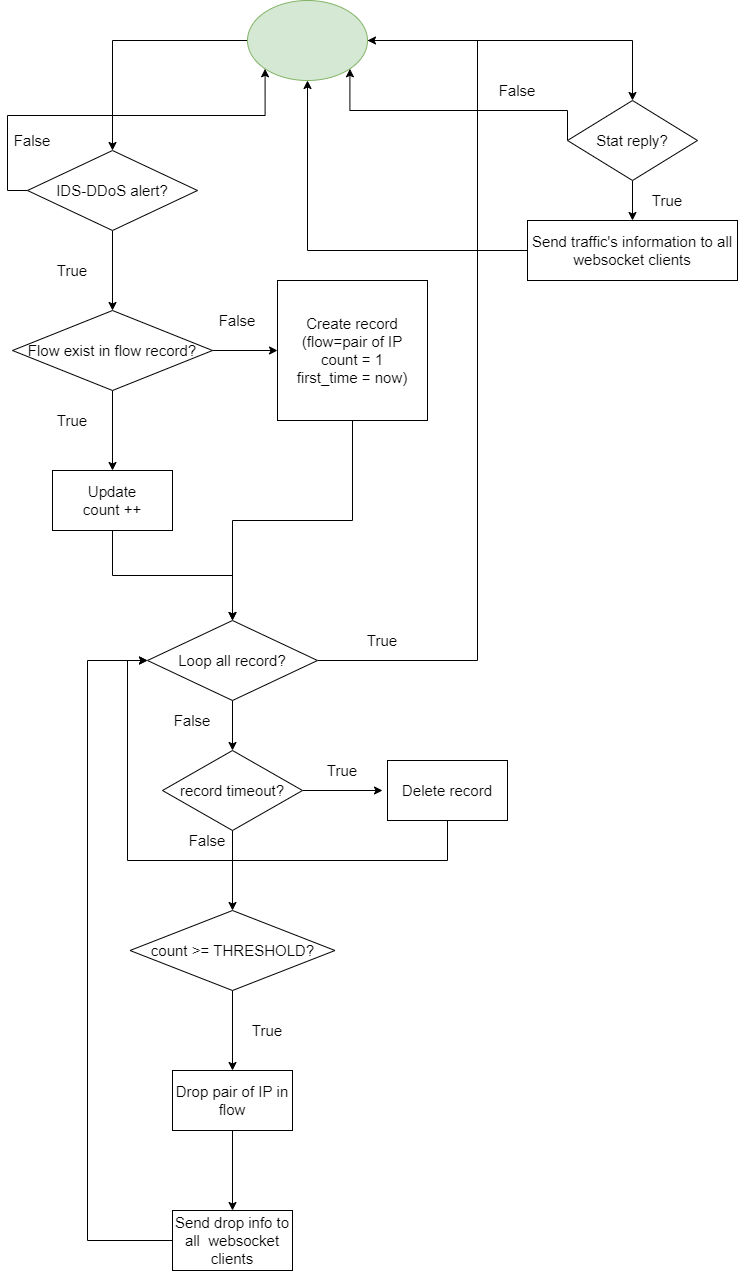
\includegraphics[width=0.75\linewidth]{fig/sdn-controller.png}
	\caption{Lưu đồ của SDN controller}
	\label{fig:sdn-controller}
\end{figure}

SDN controller sẽ tạo ra 2 server

\begin{itemize}
	\item [--] Server unixsocket để chờ tín hiệu từ IDS-DDoS.
	\item [--] Server websocket để gửi tín hiệu đến phần mềm trực quan ở máy khách.
\end{itemize}

Khi nhận được luồng có định dạng là "IP1-IP2" từ IDS-DDoS, trong đó IP1 và IP2 là IP của 2 máy cần phải chặn không cho giao tiếp, controller sẽ tiến hành kiểm tra xem cặp IP này đã được ghi nhận trong bản ghi chưa, nếu chưa thì tạo, nếu có rồi thì cập nhật trạng thái số lượng. Sau đó, controller sẽ tiến hành quét tất cả các luồng trong bản ghi, nếu luồng nào đã timeout (thời gian hiện tại trừ first\_time lớn hơn 1 hằng số giây định trước) thì xóa luồng đó, ngược lại sẽ đi kiểm tra xem luồng tấn công này có được ghi nhận lớn hơn 1 ngưỡng hằng số định trước hay không, nếu có thì chặn luồng này và gửi thông tin này đến tất cả các client đang kết nối vào websocket server, nếu không thì quay lại tiếp tục lắng nghe tín hiệu từ IDS-DDoS.

Tương tự, khi nhận được tín hiệu thống kê lưu lượng từ Open vSwitch, controller sẽ tiến hành broadcast đến tất cả client đang kết nối đến websocket server thông tin này.

Bên cạnh đó, tôi thiết kế một trang web kết nối đến websocket server để trực quan hóa các thông tin chặn luồng, lưu lượng mạng như trình bày ở trên. Hình \ref{fig:webclient-interface} thể hiện giao diện của trang web này.

\begin{figure}[ht!]
	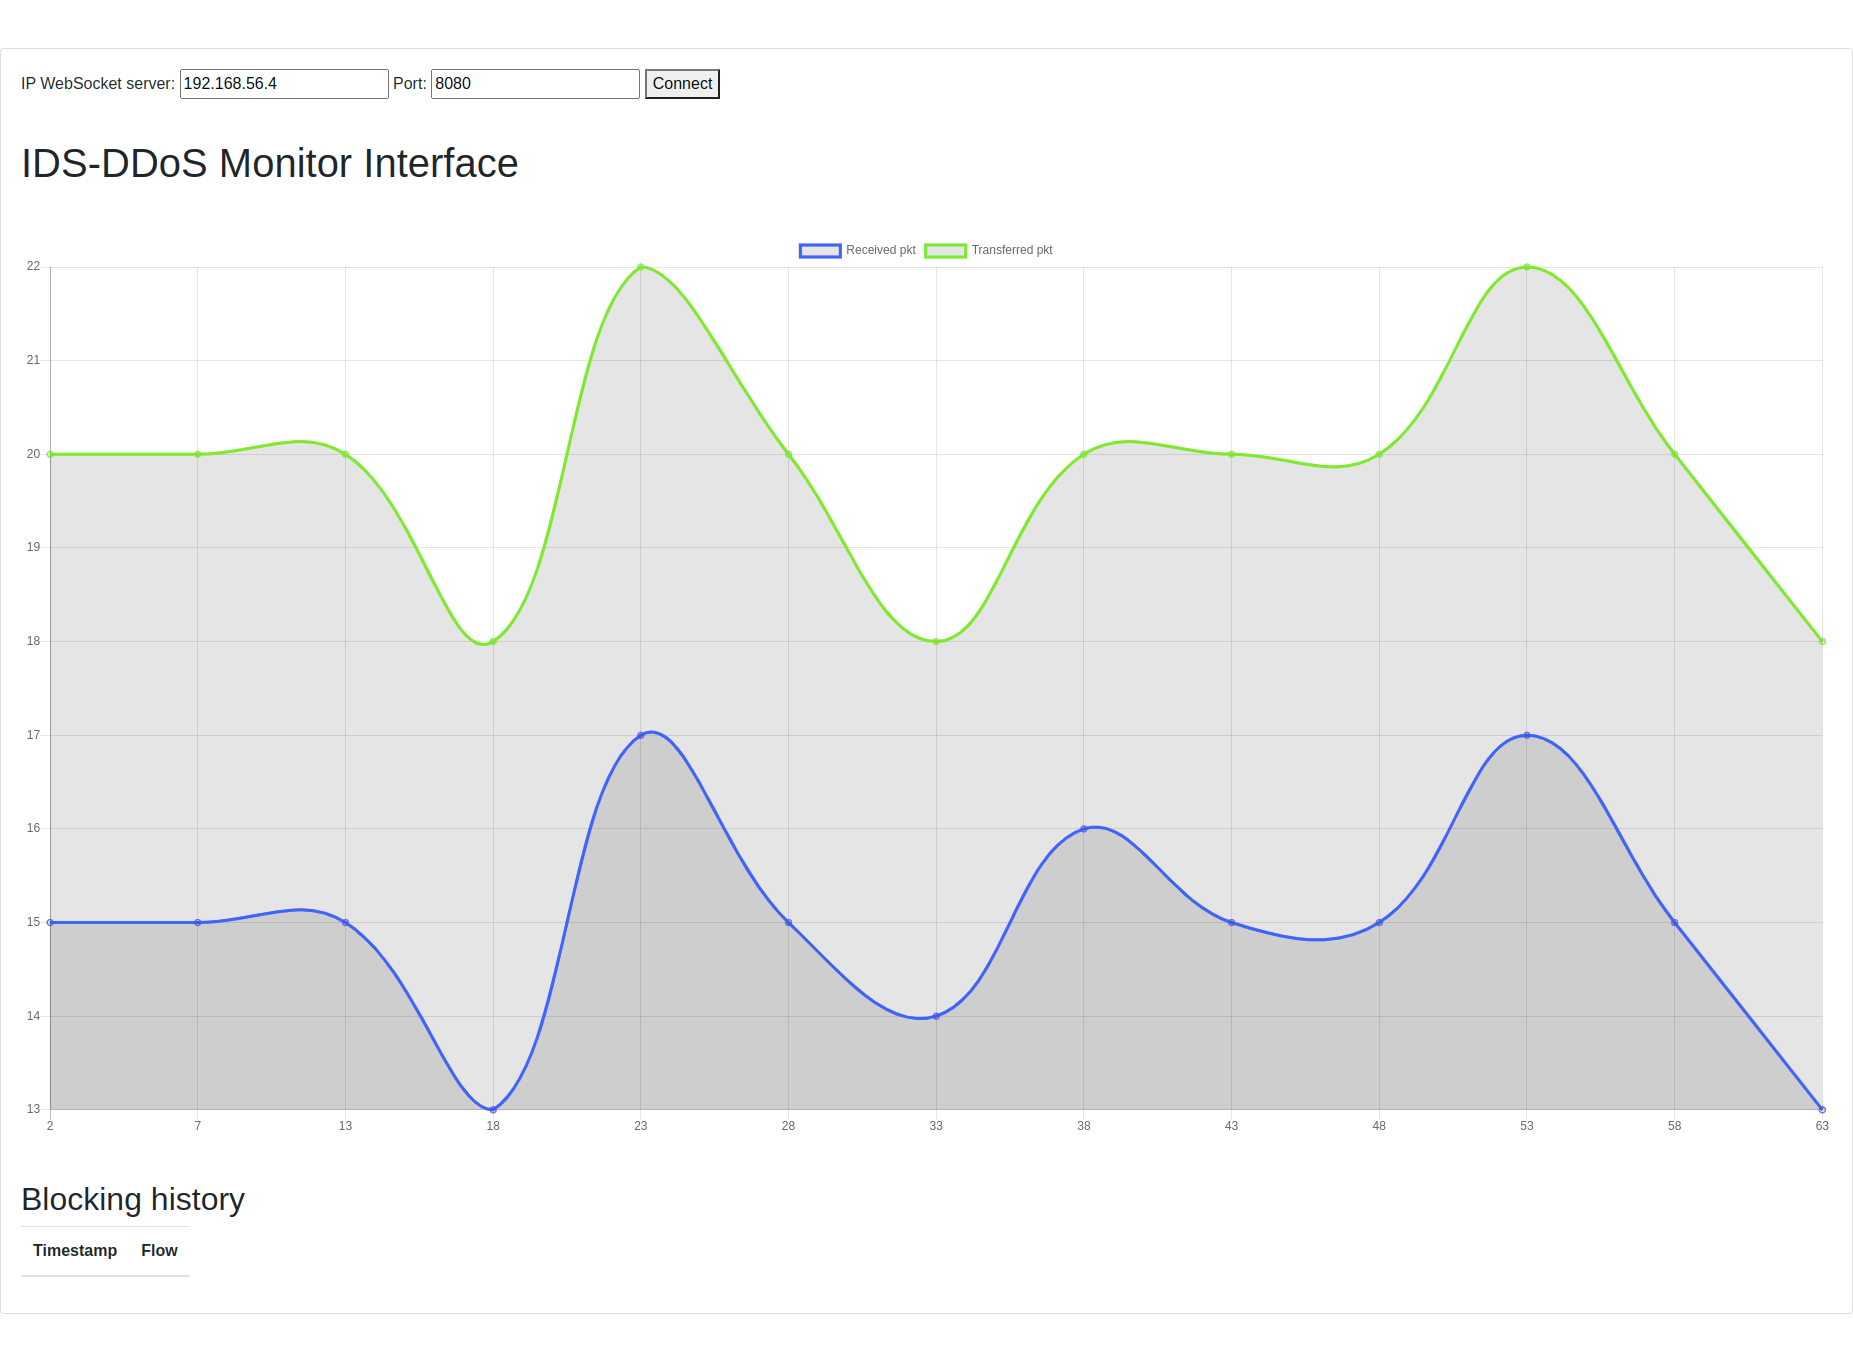
\includegraphics[width=\linewidth]{fig/webclient-interface.png}
	\caption{Giao diện web client thống  kê lưu lượng}
	\label{fig:webclient-interface}
\end{figure}

Trong đó,

\begin{itemize}
	\item [--] Trục tung là số lượng gói tin.
	\item [--] Trục hoành là thời điểm kể từ khi truy cập vào công cụ theo dõi.
	\item [--] Đường màu xanh lá biểu diễn số lượng gói tin được gửi từ trong mạng SDN ra ngoài.
	\item [--] Đường màu xanh dương biểu diễn số lượng gói tin mạng SDN nhận từ bên ngoài.
	\item [--] Bảng "Blocking history" ghi lại các cặp IP đã chặn.
\end{itemize}

\chapter{Mô hình mạng thử nghiệm}
\label{chap:network_model}
Để tạo mô phỏng các máy tính trong mạng tôi sử dụng 3 máy ảo với phần mềm Virtualbox.

Mạng mô phỏng được biểu diễn như trong hình \ref{fig:network-model}.

\begin{figure}[ht!]
	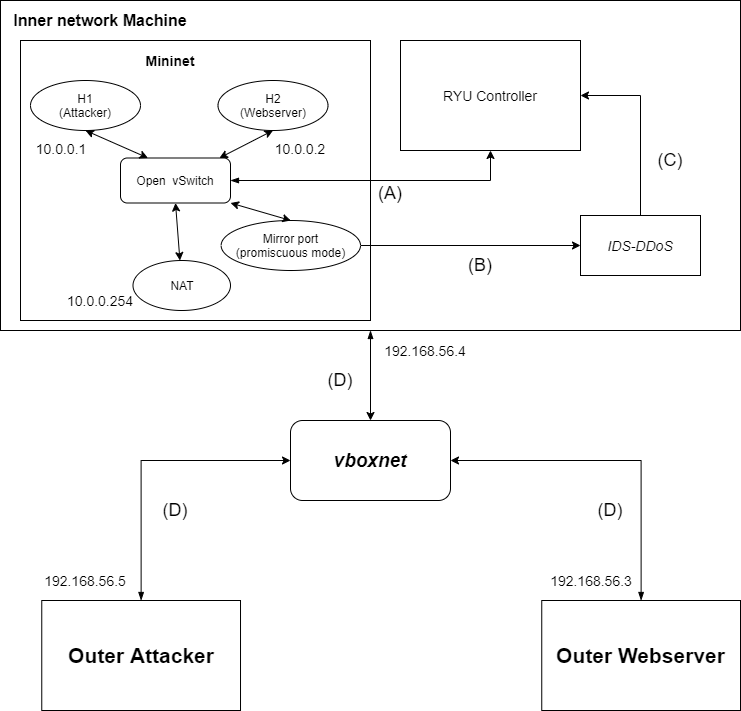
\includegraphics[width=\linewidth]{fig/network-model.png}
	\caption{Mạng mô phỏng}
	\label{fig:network-model}
\end{figure}

Các máy ảo trong mạng sẽ gồm Inner Network Machine, Outer Attacker và Outter Webserver. Các máy này được nối với nhau qua 1 mạng ảo Host-only (D) của Virtualbox với địa chỉ đường mạng là 192.168.56.0. Thông tin về các máy này được ghi trong bảng \ref{tab:host-description}.

\begin{table}[ht!]
	\begin{tabular}{|l|l|l|l|}
		\hline
		\multicolumn{1}{|c|}{\textbf{Máy}} &
		\multicolumn{1}{c|}{\textbf{Vai trò}} &
		\multicolumn{1}{c|}{\textbf{Địa chỉ IP}} &
		\multicolumn{1}{c|}{\textbf{Cấu hình}} \\ \hline
		Inner Network Machine &
		\begin{tabular}[c]{@{}l@{}}Chứa   mạng ảo \\ SDN được tạo \\ bằng Mininet, \\ RYU SDN \\ Controller và phần \\ mềm IDS-DDoS.\end{tabular} &
		192.168.56.4 &
		\begin{tabular}[c]{@{}l@{}}HĐH Ubuntu \\ 18.04 64bit\\ CPU 6 threads\\ RAM 4GB\end{tabular} \\ \hline
		Outer Webserver &
		\begin{tabular}[c]{@{}l@{}}Chứa   một trang \\ web tĩnh tạo vởi\\ SimpleHTTP \\ python\end{tabular} &
		192.168.56.3 &
		\begin{tabular}[c]{@{}l@{}}HĐH Ubuntu \\ server 18.04   32bit\\ CPU 1 thread\\ RAM 1GB\end{tabular} \\ \hline
		Outer Attacker &
		\begin{tabular}[c]{@{}l@{}}Dùng   để chạy\\ công cụ tấn công\\ DDoS Hoic\end{tabular} &
		192.168.56.5 &
		\begin{tabular}[c]{@{}l@{}}HĐH Windows 7 \\ 32bit\\ CPU 2 threads\\ RAM 2GB\end{tabular} \\ \hline
	\end{tabular}
\caption{Mô tả các máy tính trong mạng}
\label{tab:host-description}
\end{table}

\textit{Inner network Machine}

\begin{itemize}
	\item [--] Mạng SDN được kết nối 2 chiều với RYU Controller thông qua TCP localhost (A).
	\item [--] Mirror port là 1 card mạng ảo ở chế độ promiscious dùng để chuyển tất cả traffic từ H1 và H2 vào đây. Card mạng này được phần mềm IDS-DDoS lắng nghe để bắt các gói tin và phân loại luồng (B).
	\item [--] RYU Controller và phần mềm IDS-DDoS giao tiếp với nhau thông qua unixsocket (C).
\end{itemize}

\textit{Mạng SDN}

\begin{itemize}
	\item [--] H1, H2 là các host trong mạng SDN. Trong đó H1 dùng để chạy phần mềm tấn công DDoS Hulk, H1 dùng để làm 1 webserver. 
	\item [--] Để H1, H2 có thể giao tiếp với bên ngoài, Open vSwitch được trang bị thêm 1 thiết bị NAT.
	\item [--] Ngược lại, để máy bên ngoài có thể giao tiếp với Webserver H2, các lệnh ''iptables nat'' được dùng sao cho tất cả gói tin đi tới  port 80 của máy  Inner network machine sẽ được chuyển vào port 80 của thiết bị NAT trong SDN, từ đó, tất cả các gói tin đi vào port 80 sẽ được chuyển vào port 80 của máy H2. Mô hình như hình \ref{fig:nat}.
\end{itemize}

\begin{figure}[ht!]
	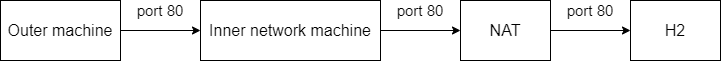
\includegraphics[width=\linewidth]{fig/nat.png}
	\caption{Mô hình NAT port}
	\label{fig:nat}
\end{figure}

\chapter{Thử nghiệm và phân tích kết quả}
\label{chap:testing}
Trong chương này, tôi sẽ xây dựng hai kịch bản để kiểm thử hoạt động của phần mềm  IDS-DDoS trong mạng SDN. Hai kịch bản này là:

\begin{itemize}
	\item [--] Mạng SDN bị tấn công từ bên ngoài. Kịch bản này tương tự như các kịch bản tấn công mạng thường gặp. Trong trường hợp này, tôi sẽ sử dụng IDS-DDoS để cố gắng bảo vệ và giảm thiểu thiệt hại cho hệ thống mạng cũng như máy chủ web bên trong.
	\item [--] Máy con trong mạng SDN bị lợi dụng tấn công ra bên ngoài. Kịch bản này tương tự như kịch bản các thiết bị IoT bị xâm nhập và trở thành botnet. Trong trường hợp này, tôi sẽ cố gắng ngăn chặn các thiết bị bên trong mạng SDN thực hiện tấn công đến các máy chủ bên ngoài.
\end{itemize}

Với phần  mềm IDS-DDoS, tôi sử dụng mô hình LSVM để nhận diện các luồng tấn công. Mặc dù kết quả huấn luyện cho thấy LSVM có độ chính xác thấp hơn so với Decision Tree, Random Forest hay DNN (mục \ref{compare-multi-models}), tuy nhiên, khi áp dụng thực tế, LSVM lại nhận diện luồng tấn công tốt hơn. Kết luận này được tôi rút ra từ việc quan sát quá trình hoạt động của các mô hình trong môi trường thực nghiệm, phần này sẽ được tôi trình bày trong phần \ref{test-conclusion}.

Các biểu đồ trong mục này được chụp từ công cụ theo dõi lưu lượng gói tin trong mạng được thiết kế trong mục \ref{traffic-monitor}.

\section{Mạng SDN bị tấn công từ bên ngoài}
\label{c:6.1}

Trong kịch bản này, Outer Attacker sẽ sử dụng công cụ HOIC để tấn công vào Webserver H2.

Giao diện công cụ HOIC trong hình \ref{fig:hoic}. Vì đây là công cụ không dành cho học thuật và có thể bị lợi dụng để sử dụng với mục đích xấu  nên tôi không chỉ ra nơi tham khảo hay cách tải xuống công cụ này.

\begin{figure}[ht!]
	\centering
	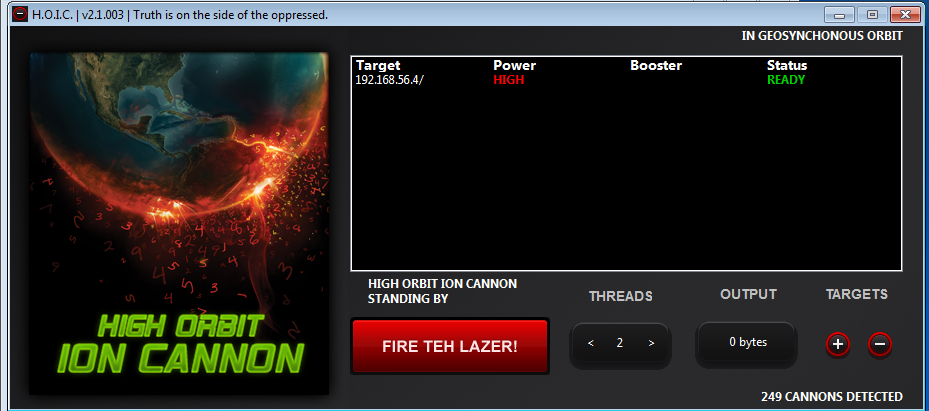
\includegraphics[width=0.75\linewidth]{fig/hoic.png}
	\caption{Giao diện công cụ HOIC}
	\label{fig:hoic}
\end{figure}

Quá trình tấn công được biểu thị trong các biểu đồ dưới đây.

Biểu đồ trong hình \ref{fig:B1} mô tả trạng thái mạng trước và trong lúc bị tấn công. 

Lúc đầu, nhìn theo trục gói tin, ta thấy được số lượng gói tin đến và gói tin đi vẫn còn thấp. Đường màu xanh lá biểu diễn số lượng gói tin đi, tức là các gói tin được phản hồi từ máy chủ web H2. Đường màu xanh dương biểu thị gói tin đến, tức là các gói tin được gửi tử Outer attacker.

Tuy nhiên, khi tấn công diễn ra, ta thấy được số lượng gói tin đến và đi tăng lên đột ngột trong một khoảng thời gian. Sau đó, số lượng gói tin đi (đường xanh lá) giảm xuống 0, trong khi số lượng gói tin đến (đường xanh dương) vẫn tăng. Nguyên nhân là do khi IDS-DDoS phát hiện tấn công và thông báo cho SDN  controller chặn luồng IP, lúc này, máy chủ H2 bên trong mạng không thể nhận thêm yêu cầu từ attacker nên không thể phản hồi, trong khi đó attacker vẫn tiếp tục tấn công làm cho số lượng gói tin đến tăng không ngừng.

\begin{figure}[ht!]
	\centering
	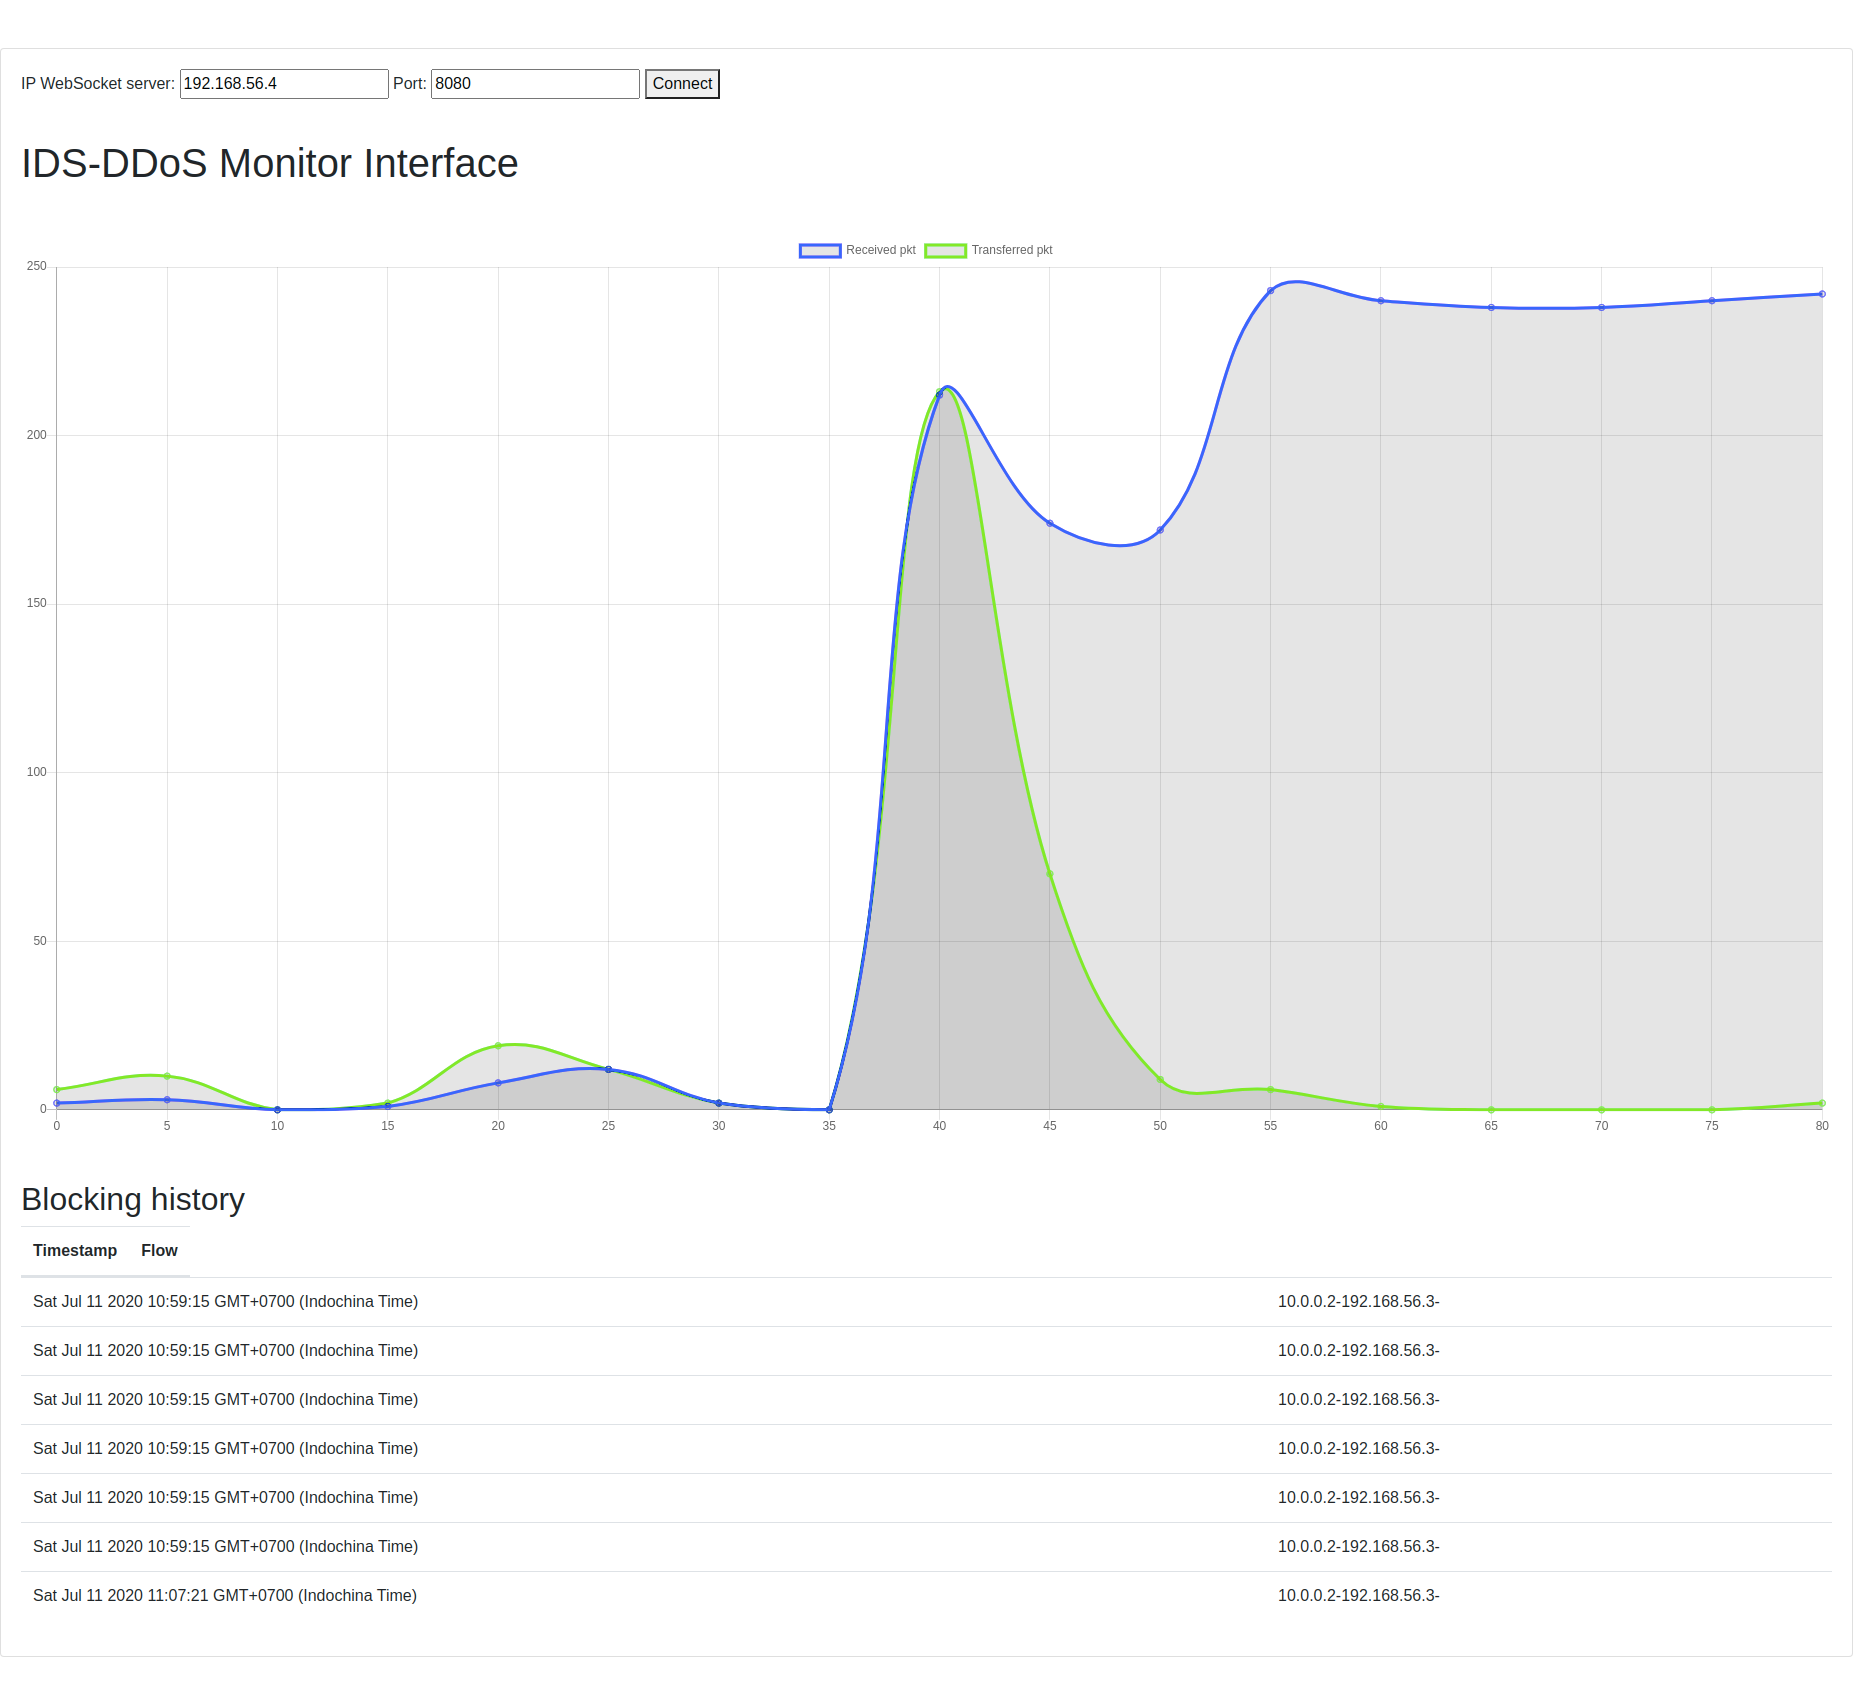
\includegraphics[width=\linewidth]{fig/B1.png}
	\caption{Kịch bản 1: Trạng thái mạng trước và trong khi tấn công}
	\label{fig:B1}
\end{figure}

Sau khi kết thúc tấn công (hình \ref{fig:B2}), số lượng gói tin đến và đi đều giảm xuống 0.

\begin{figure}[ht!]
	\centering
	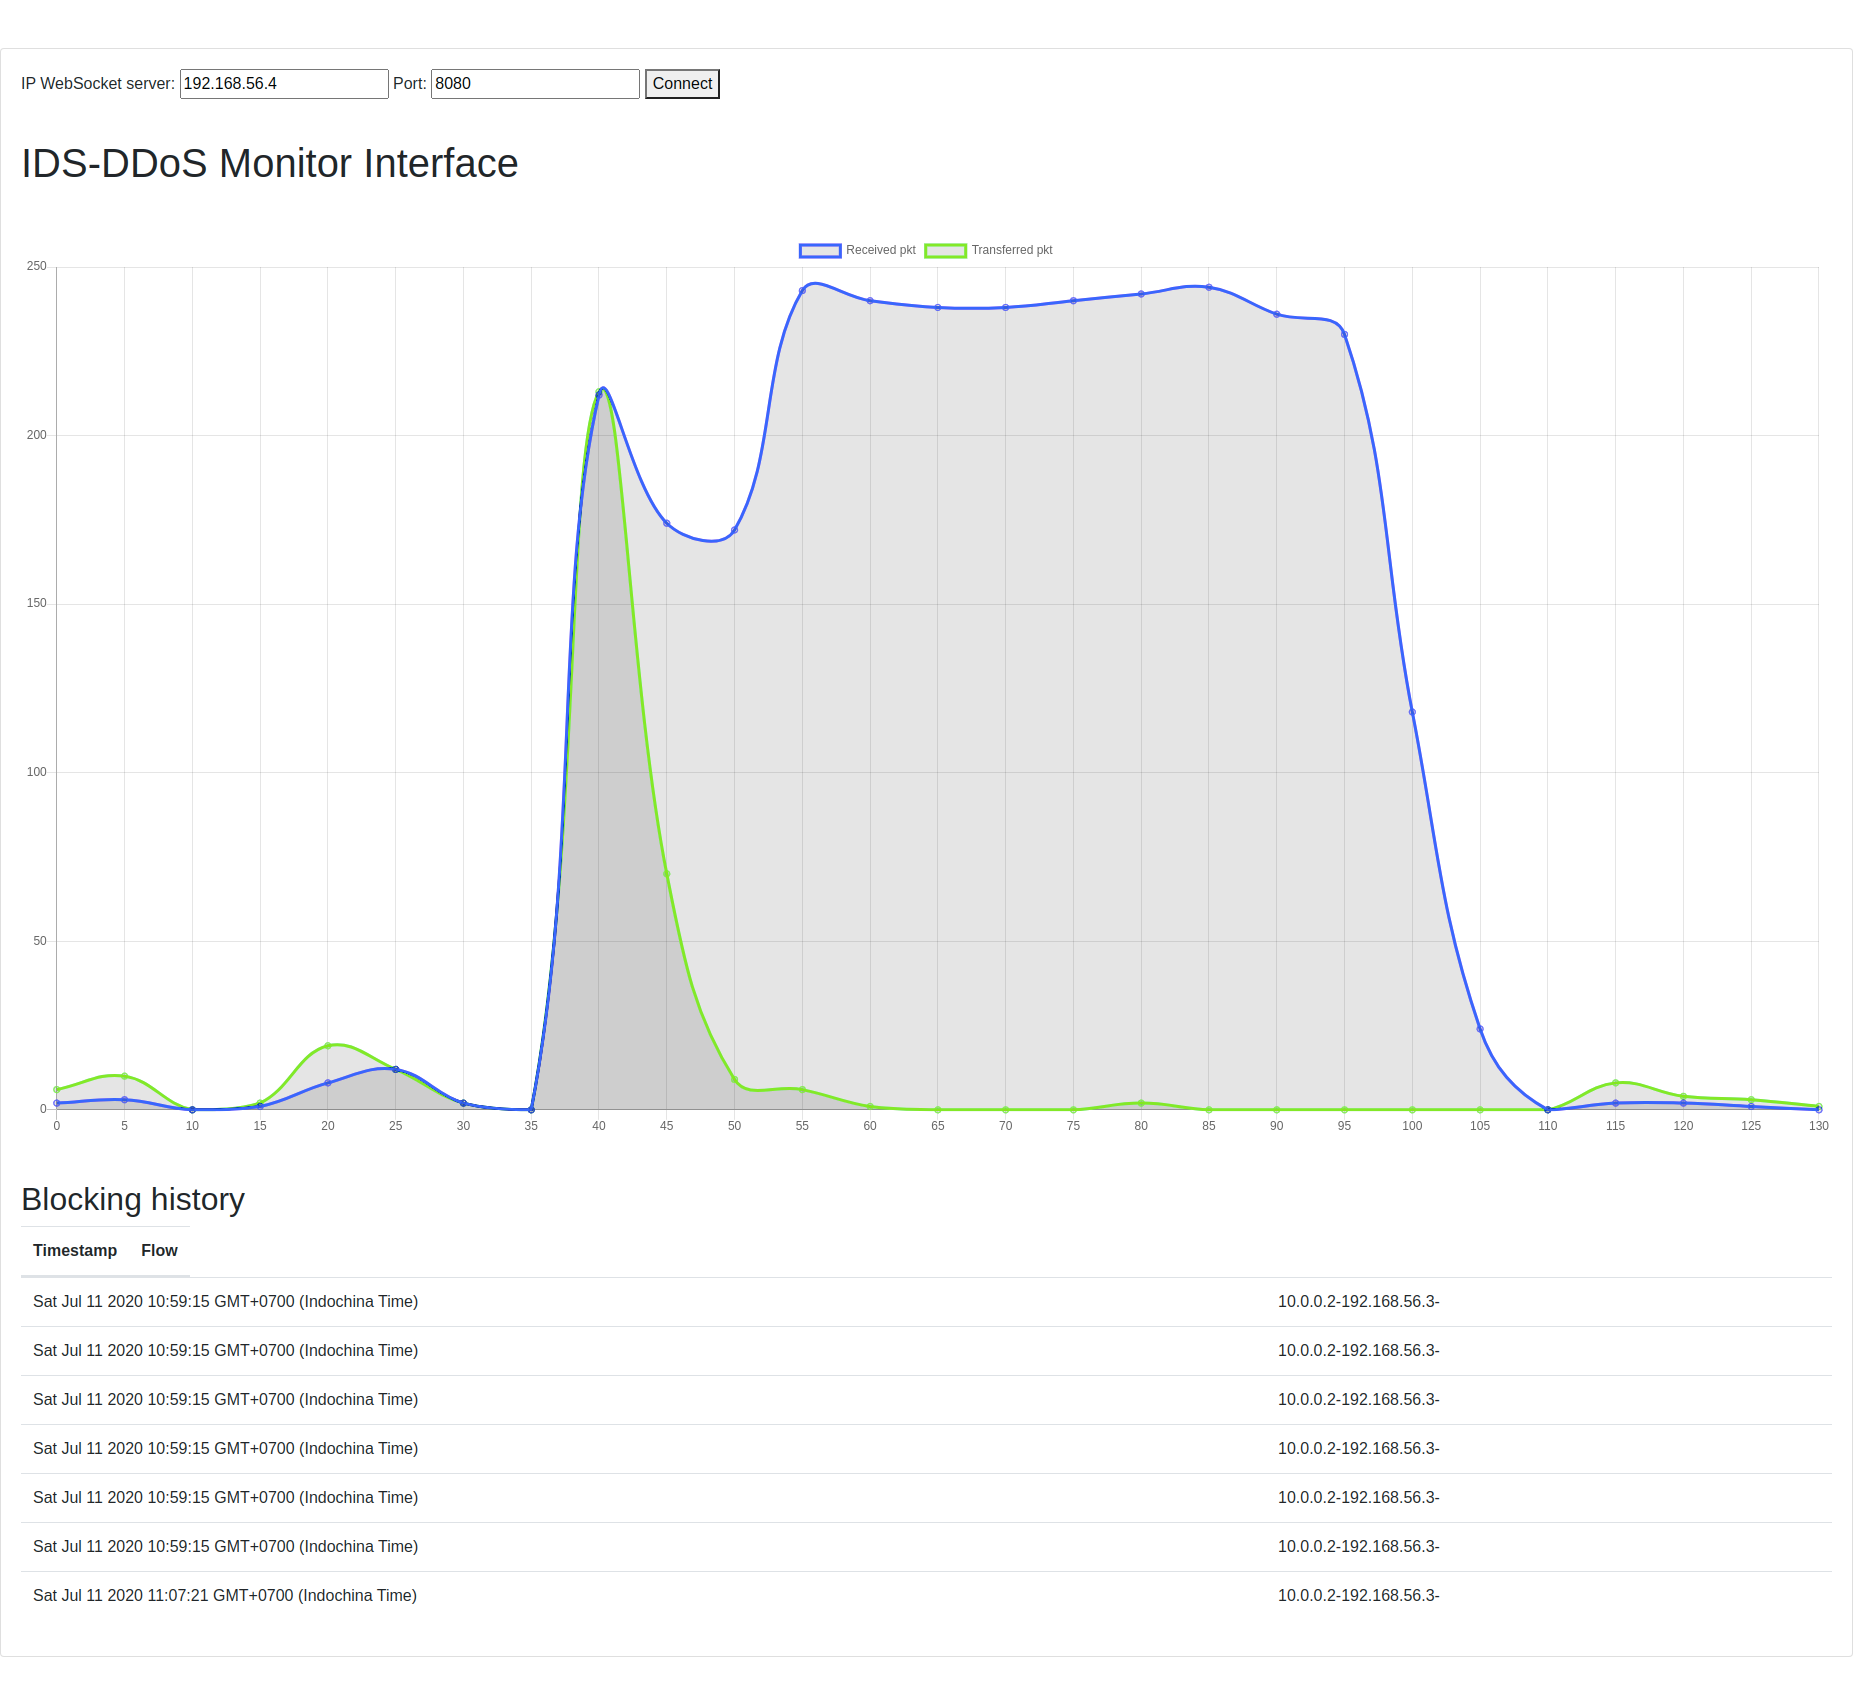
\includegraphics[width=\linewidth]{fig/B2.png}
	\caption{Kịch bản 1: Trạng thái mạng sau khi tấn công}
	\label{fig:B2}
\end{figure}

\section{Máy con trong mạng SDN bị lợi dụng tấn công ra bên ngoài}

Trong kịch bản này attacker H1 sẽ tấn công vào Outer Webserver bằng công cụ Hulk.

Hulk là công cụ giao diện console, với cùng lý do nêu trong mục \ref{c:6.1}, tôi cũng sẽ không chia sẽ cách tiếp cận công cụ này.

Quá trình tấn công được biểu thị trong biểu đồ \ref{fig:C1} dưới đây.

Lúc đầu, nhìn theo trục gói tin, ta thấy được số lượng gói tin đến và gói tin đi vẫn còn thấp.

Đường màu xanh dương biểu diễn gói tin đến, tức là các gói tin phản hồi từ Outer Webserver. Đường màu xanh lá biểu diễn gói tin đi, tức là các gói tin được gửi từ Attacker H1.

\begin{figure}[ht!]
	\centering
	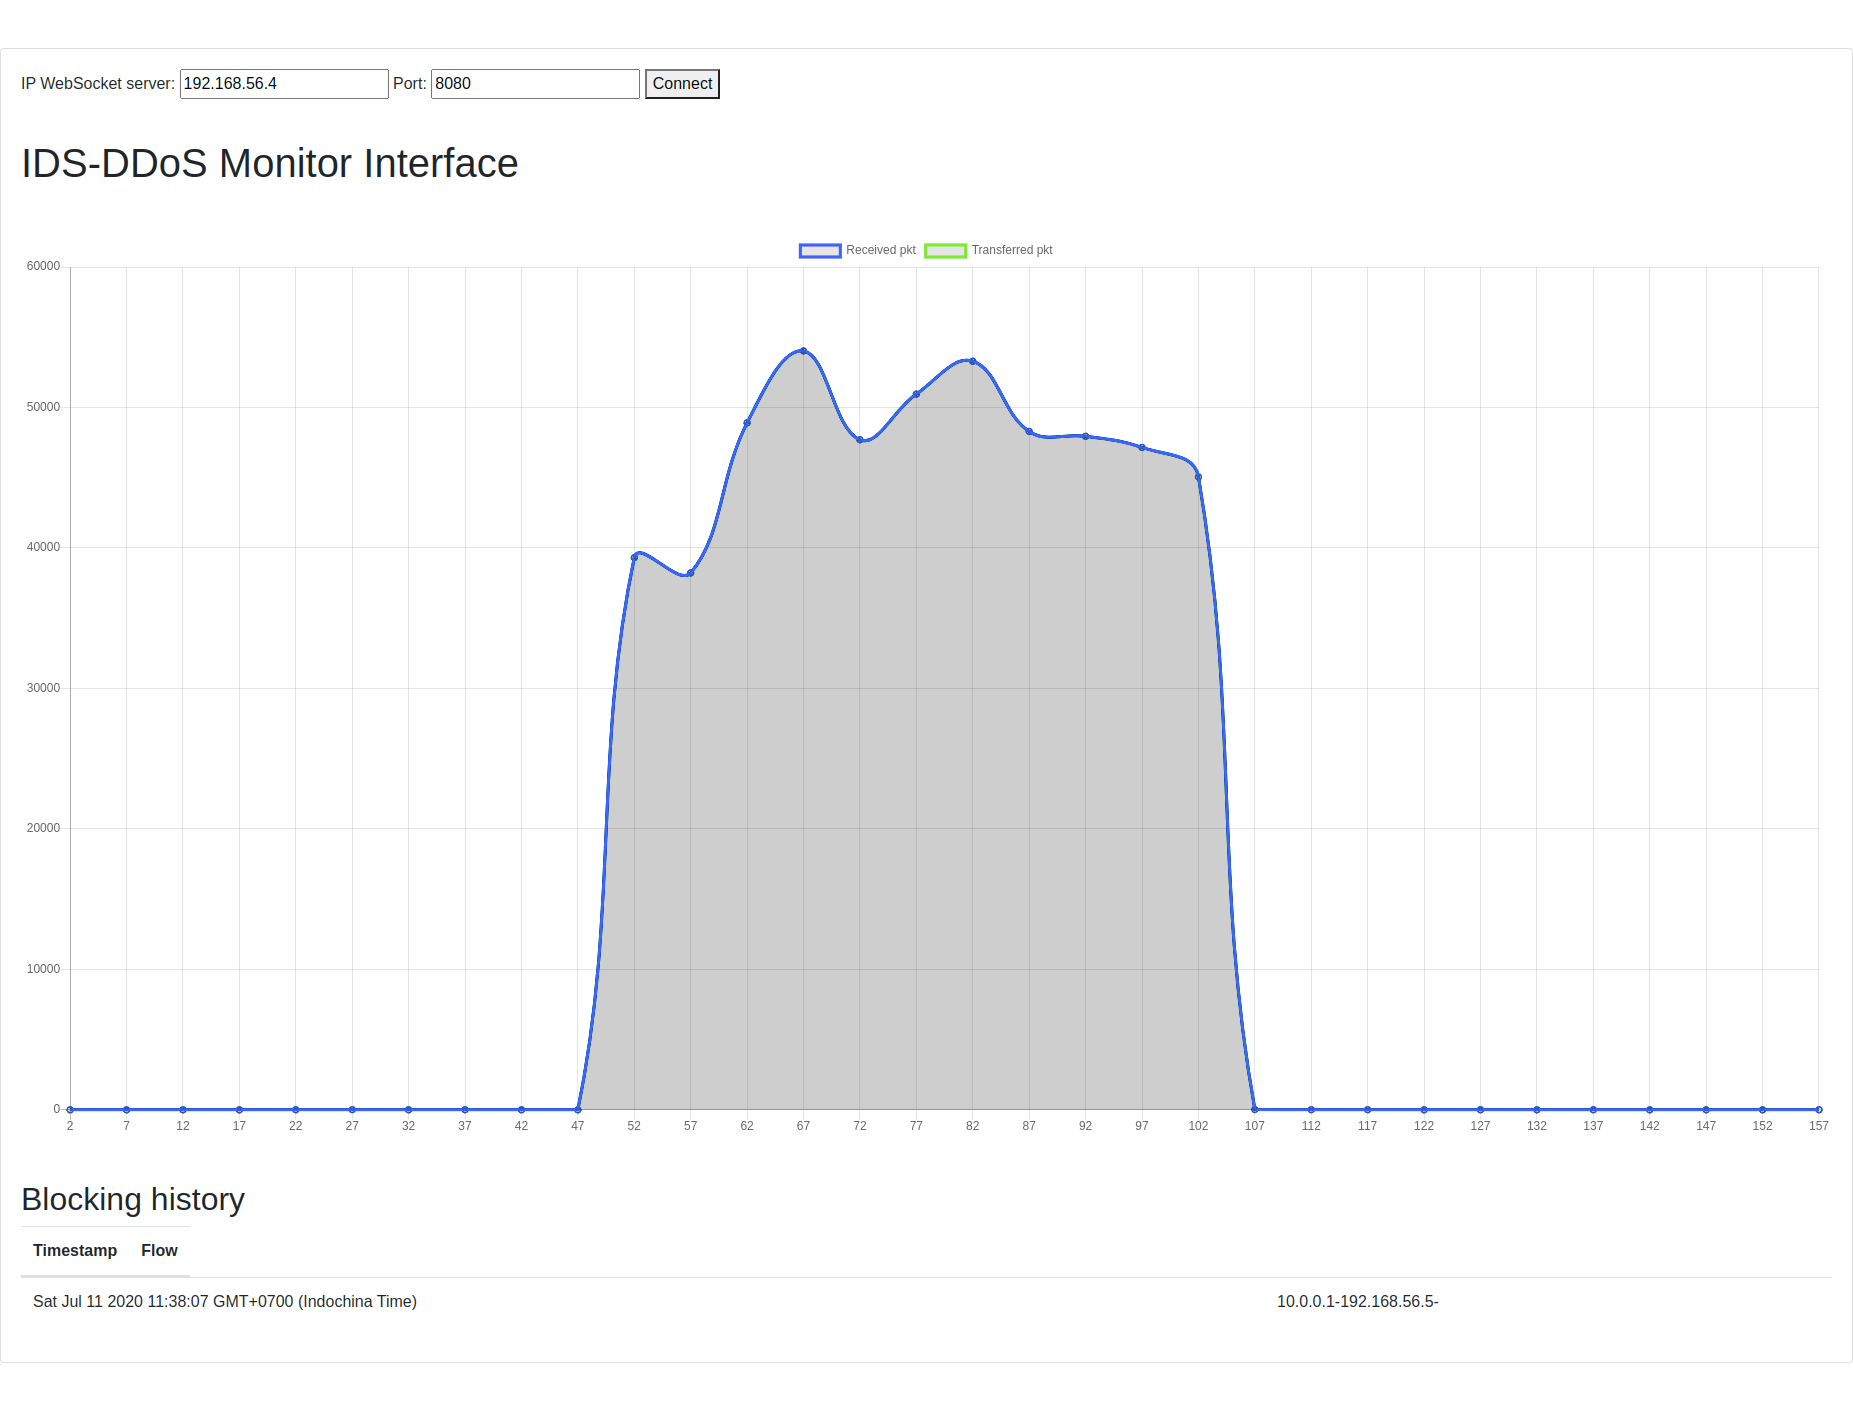
\includegraphics[width=\linewidth]{fig/C1.png}
	\caption{Kịch bản 2: Trạng thái mạng trong quá trình H1 tấn công}
	\label{fig:C1}
\end{figure}

Tuy nhiên, khi H1 bắt đầu tấn công, ta thấy số lượng gói tin đến và đi tăng lên đột ngột và tăng rất cao. Tuy nhiên sau một khoảng thời gian, số lượng gói tin này giảm xuống còn 0. Lý do là vì khi IDS-DDoS phát hiện tấn công và thông báo cho SDN controller để chặn luồng IP, cho nên H1 không thể tiếp tục tạo các kết nối đến Outer Webserver. Bên cạnh đó, H1 là máy con trong mạng SDN, nên các gói tin bị chặn tại nguồn tấn công, ta không thể quan sát được số lượng gói tin đi (đường xanh lá) tiếp tục tăng như trong kịch bản \ref{c:6.1} dù cho H1 vẫn tiếp tục tấn công.

\section{Kết luận kết quả kiểm thử}
\label{test-conclusion}

Từ hai kịch bản thí nghiệm trên, tôi nhận thấy phần mềm IDS-DDoS có khả năng nhận diện và phòng thủ trước tấn công DDoS. Tuy nhiên, khi so sánh giữa hai biểu đồ \ref{fig:B1} và \ref{fig:B2}, tôi nhận thấy, phần mềm không nhận diện tốt được các luồng tấn công từ công cụ Hulk.

Tôi đã tìm hiểu nguyên nhân và phát hiện ra rằng, trong dataset CICIDS2018 mà tôi sử dụng ở mục \ref{ids-dataset}, các luồng tấn công Hulk mà tác giả ghi nhận rất khác so với luồng tấn công do công cụ Hulk được tôi sử dụng. Trong đó, các gói tin và thời gian của luồng mà công cụ Hulk do tôi sử dụng sẽ nhỏ hơn nhiều so với tác giả. Lý do này đã khiến cho công cụ IDS-DDoS bị nhầm lẫn hầu hết các luồng tấn công Hulk là luồng hợp lệ. Thử nghiệm với mô hình học sâu DNN, tôi cũng được kết quả tương tự.

Ngoài ra, khi áp dụng các mô hình vào phần mềm IDS-DDoS trong môi trường thực nghiệm, tôi nhận ra vấn đề về khả năng nhận diện tấn công của các mô hình trong khi huấn luyện và trên thực tế là khá khác nhau.

Để xấy dựng môi trường thực nghiệm, tôi thiết kế một mạng gồm hai máy ảo, một máy đóng vai trò là ''attacker'' một máy đóng vai trò là ''victim''. Trên máy victim tôi cài đặt phần mềm IDS-DDoS để nhận diện tấn công. Sau đó, tôi sử dụng công cụ HOIC để thực hiện giả lập tấn công DDoS từ máy attacker sang máy victim. 

Trong lúc thực nghiệm, mô hình Naive Bayes cho kết quả tệ nhất các luồng tấn công và luồng thông thường bị nhận diện nhầm rất nhiều. Tuy nhiên điều làm tôi ngạc nhiên là mặc dù có độ chính xác cao với kiến trúc đơn giản nhưng Decision Tree và Random Forest lại thể hiện khả năng nhận diện tấn công rất kém, hầu hết các luồng tấn công đều được nhận diện là luồng thông thường. Trong khi đó, mô hình LinearSVM và DNN tuy có các tiếp cận phức tạp hơn và độ chính xác không cao bằng, nhưng lại nhận diện rất tốt các luồng tấn công.




\chapter{Tổng kết}
\label{chap:conclusion}
Qua 6 chương trước đó tôi đã lần lượt trình bày quá trình tìm hiểu và cài đặt công cụ phát hiện và phòng thủ trước tấn công DoS/DDoS trong mạng SDN của mình. Chương này tổng kết lại những điểm được và chưa được của khóa luận này và đưa ra những hướng phát triển nếu có thể trong tương lai.

\section{Các kết luận từ đề tài}

Từ kết luận ở mục \ref{compare-multi-models} và mục \ref{test-conclusion},  tôi rút ra  được các ý sau.

\begin{itemize}
	\item [--] Đối với dataset CICIDS2018, mô hình có cách tiếp cận đơn giản nhưng  mang lại kết quả tốt nhất là Decision Tree.
	\item [--] Khi áp dụng vào thực nghiệm, độ chính xác của mô hình khi huấn luyện lại khác xa so với thực tế. Ở đây, mô hình Decision Tree lại thể hiện khả năng nhận diện kém hơn LinearSVM.
	\item [--] Các mô hình hiện tại sẽ bị vô hiệu trước một mẫu tấn công mới, hoàn toàn xa lạ. Điều này có thể  rút ra từ phần kiểm thử với công cụ Hulk, khi mà công cụ tôi sử dụng hoạt động khác so với công cụ mà tác giả của dataset CICIDS2018 sử dụng.
	\item [--] Công cụ tôi phát triển không nên sử dụng độc lập mà cần kết hợp với nhiều công cụ sử dụng các kỹ thuật khác để tăng độ chính xác và độ tin cậy.
\end{itemize}

\section{Kết quả đạt được}

\textbf{Những điều làm được}:

\begin{itemize}
	\item [--] Hiểu được các cách thức và nguy cơ của tấn công DoS/DDoS hiện nay.
	\item [--] Hiểu và ứng dụng các mô hình học máy Linear SVM, Naïve Bayes, Decision Tree, Random Forest và mô hình học sâu để giải quyết vấn đề phân loại luồng gói tin.
	\item [--] Huấn luyện được  nhiều  mô hình học máy và tìm được mô hình đơn giản mà hiệu quả là Decision Tree.
	\item [--] Hoàn thành proof-of-concept công cụ phát hiện tấn công DoS/DDoS  theo thời gian thực (IDS-DDoS).
	\item [--] Hoàn thành proof-of-concept hệ thống mạng SDN mô phỏng quá trình tấn công và phòng thủ với hai kịch bản thường gặp.
\end{itemize}

\textbf{Những điều chưa làm được}:

\begin{itemize}
	\item [--] Chưa huấn luyện được một số mô hình học sâu do hạn chế về khả năng xử lý dữ liệu, do kích thước dữ liệu quá lớn.
	\item [--] Chưa kiểm tra chéo mô hình trên các tập dữ liệu khác nhau do nhiều nguyên nhân như bất đồng về định dạng của các tập dữ liệu, kích thước tập dữ liệu quá lớn, vv.
\end{itemize}

\section{Hướng phát triển}

\begin{itemize}
	\item [--] Huấn luyện thêm một số mô hình học sâu.
	\item [--] Kiểm tra chéo kết quả các mô hình trên các tập dữ liệu khác nhau.
	\item [--] Áp dụng và đánh giá công cụ IDS-DDoS vào một số nền tảng mạng khác so với SDN.
	\item [--] Tìm ra nguyên nhân vì sao độ chính xác khi huấn luyện lại khác so với thực nghiệm.
	\item [--] Tìm một mô hình học máy hay học sâu tốt hơn để có thể nhận diện được công cụ tấn công không nằm trong  dataset.
	\item [--]  Kết hợp công cụ IDS-DDoS với các công cụ khác để tăng độ tin cậy và độ chính xác.
\end{itemize}

\section{Lời kết}

Trong thời gian có hạn, tôi chỉ mới nghiên cứu được một phần trong lĩnh vực phòng chống tấn công DoS/DDoS cũng như công nghệ SDN.

Có thể những kiến thức tôi thu nhận được trong thời gian qua chưa đủ nhiều. Tuy nhiên tôi nhận thấy mình đã phát triển được những kỹ năng như: kỹ năng tìm kiếm thông tin, kỹ năng phân tích và giải quyết vấn đề, khả năng thích nghi với môi trường và công nghệ mới, vv. Với những kỹ năng thu được, tôi hi vọng sẽ giúp tôi phát triển hơn trong tương lai.

Mặc dù đã cố gắng trong quá trình thực hiện, chắc chắn khóa luận không tránh
khỏi những thiếu sót. Rất mong nhận được sự góp ý và chỉ bảo tận tình của quý thầy
cô và các bạn.

\bibliography{thesis}{}
\bibliographystyle{ieeetr}
\end{document}
